\documentclass[]{tufte-book}

% ams
\usepackage{amssymb,amsmath}

\usepackage{ifxetex,ifluatex}
\usepackage{fixltx2e} % provides \textsubscript
\ifnum 0\ifxetex 1\fi\ifluatex 1\fi=0 % if pdftex
  \usepackage[T1]{fontenc}
  \usepackage[utf8]{inputenc}
\else % if luatex or xelatex
  \makeatletter
  \@ifpackageloaded{fontspec}{}{\usepackage{fontspec}}
  \makeatother
  \defaultfontfeatures{Ligatures=TeX,Scale=MatchLowercase}
  \makeatletter
  \@ifpackageloaded{soul}{
     \renewcommand\allcapsspacing[1]{{\addfontfeature{LetterSpace=15}#1}}
     \renewcommand\smallcapsspacing[1]{{\addfontfeature{LetterSpace=10}#1}}
   }{}
  \makeatother

\fi

% graphix
\usepackage{graphicx}
\setkeys{Gin}{width=\linewidth,totalheight=\textheight,keepaspectratio}

% booktabs
\usepackage{booktabs}

% url
\usepackage{url}

% hyperref
\usepackage{hyperref}

% units.
\usepackage{units}


\setcounter{secnumdepth}{2}

% citations


% pandoc syntax highlighting

% table with pandoc
\usepackage{longtable,booktabs,array}
\usepackage{calc} % for calculating minipage widths
% Correct order of tables after \paragraph or \subparagraph
\usepackage{etoolbox}
\makeatletter
\patchcmd\longtable{\par}{\if@noskipsec\mbox{}\fi\par}{}{}
\makeatother
% Allow footnotes in longtable head/foot
\IfFileExists{footnotehyper.sty}{\usepackage{footnotehyper}}{\usepackage{footnote}}
\makesavenoteenv{longtable}

% multiplecol
\usepackage{multicol}

% strikeout
\usepackage[normalem]{ulem}

% morefloats
\usepackage{morefloats}


% tightlist macro required by pandoc >= 1.14
\providecommand{\tightlist}{%
  \setlength{\itemsep}{0pt}\setlength{\parskip}{0pt}}

% title / author / date
\title{Decision Theory}
\author{Bert Baumgaertner}
\date{2022-09-09}

\usepackage{booktabs}
\usepackage{amsthm}
\makeatletter
\def\thm@space@setup{%
  \thm@preskip=8pt plus 2pt minus 4pt
  \thm@postskip=\thm@preskip
}
\makeatother
\usepackage{tikz}
\usepackage{pgfplots}

\begin{document}

\maketitle



{
\setcounter{tocdepth}{0}
\tableofcontents
}

\hypertarget{preface-and-prerequisites}{%
\chapter*{Preface and Prerequisites}\label{preface-and-prerequisites}}
\addcontentsline{toc}{chapter}{Preface and Prerequisites}

\href{decisiontheory.pdf}{Download PDF of Entire Textbook}

Many of us are familiar with the idea of making a list of ``pros'' and ``cons'' to help us make a choice, particularly important and complex ones. Presumably, this kind of strategy reflects our desire to make the ``right'' choice. Or maybe there isn't a single correct choice to make, but at least we want to examine our options so that we can provide a kind of justification for what we end up deciding to do. In other words, one purpose of a pros-and-cons list is that we can provide \emph{reasons} for our choices. Decision theory is the field that examines a whole array of decision making strategies that explain and justify choices, even if the consequences don't work out as expected.

\hypertarget{what-is-a-conceptual-introduction}{%
\section{What is a conceptual introduction?}\label{what-is-a-conceptual-introduction}}

This book is a conceptual introduction to decision theory. As such, there are several features that differentiate it from other introductions. First, while it draws heavily on philosophical approaches, many of the concepts are also informed by other disciplines. So when it will benefit our understanding of a concept, we will not hesitate to venture into areas such as psychology and economics.

Second, the concepts we cover will be used to build models of decision-making. In this sense the ``theory'' that we aspire to is not so much a thesis about what rational decision making is. Rather, our ``theory'' is more akin to a collection of tools that can be used for doing analysis. That is not to say, however, that we will eshew normative claims. We will find ourselves in plenty of places where we'll use claims about rationality and irrationality, and in turn the concepts we have will help us better understand those notions.

Third, there is a great deal of conceptual overlap between fields such as game theory, social choice theory, behavioral economics, and traditional decision theory (or decision theory ``proper''). The differences between them is largely about the domains of decision making: game theory focuses on strategic decisions between multiple agents; social choice theory is about how to aggregate preferences of individuals to the level of the collective; behavioral economics emphasizes empirical studies to develop a non-ideal decision theory; and decision theory ``proper'' is typically the idealized study of rationality and its normative consequences. But there are many concepts that appear across several of these domains. Rather than take a domain as a starting point and cover the concepts needed to understand the theories in those domains, we will start with concepts and then illustrate how they are used in some of these domains. That said, we will not aim to be exhaustive of where the concepts are used. The goal is for the reader to appreciate the utility of the concept and get a feel for its connections to domains outside traditional decision theory.

Fourth, to the end that we focus on concepts, we will start with bare bones. The concepts will be initially crude. At first we will use them to get some basic models of decision-making, many of which will resemble overly simplified (``toy model'') decisions rather than real-life decisions. Then we will advance in one of two ways. Sometimes we will advance by adding one or more new concepts and then explore how that helps us develop more sophisticated models. Other times we will refine one or more of our existing concepts and see how that changes our models and interpretations of them.

Fifth, and finally, the goal of a conceptual introduction is to maximize accessibility. That said, it will become necessary at some point that to clarify a concept we will have to use some tools of rigor. Most readers will be already familiar with most of these: how to read a table or matrix, executing basic algebraic operations like addition and multiplication, how to read a graph that plots a function, etc. Other tools, notably some basic probability theory, readers are not expected to know. We will prefer, whenever possible, to make a concept clear without the use of formal tools. Where this is not possible, the relevant representations will be introduced as if the reader is seeing them for the first time.

The most rudimentary tools we start using early on include tables and orders of operation of addition and multiplication. Readers well-versed in these may skip to the first chapter.

\hypertarget{how-to-read-a-table-or-matrix}{%
\section{How to read a table or matrix}\label{how-to-read-a-table-or-matrix}}

This books make very few assumptions about the reader's background knowledge. This book makes frequent use of tables, or sometimes called matrices (``matrix'' for a single one). So it's worth getting clear on the parts that make up a table. The basic setup is a grid, with horizontal lines (left-right) and vertical lines (up-down). Sometimes the lines aren't shown because it looks clearer. In that case we make sure to organize text in a way that lines up as a grid.

The horizontal regions are called rows and the vertical regions are columns. A cell is where a row and a column intersect. The cells in the very first row usually contains information about the names of the columns (this first row is often called a \emph{header}). The cells in the very first column typically have the names for the rows. Because the first row and first column are being used to label or name the rest of the row or column, they aren't included when we count the number of rows (or columns) of a table. Below is an example. Notice that the whole grid is made up of three rows and three columns, but because the first ones just have names, the counting starts at the second row and column of the grid.

\begin{longtable}[]{@{}lcc@{}}
\caption{Example of a two-by-two table with names for rows and columns. The name ``Row 1'' refers to the horizontal region to its right and consists of Cell(1,1) and Cell(1,2). The name ``Column 1'' refers to the vertical region below it and consists of Cell(1,1) and Cell(2,1).}\tabularnewline
\toprule
& Column 1 & Column 2\tabularnewline
\midrule
\endfirsthead
\toprule
& Column 1 & Column 2\tabularnewline
\midrule
\endhead
\textbf{Row 1} & Cell(1,1) & Cell(1,2)\tabularnewline
\textbf{Row 2} & Cell(2,1) & Cell(2,2)\tabularnewline
\bottomrule
\end{longtable}

\hypertarget{the-very-basic-math}{%
\section{The Very Basic Math}\label{the-very-basic-math}}

The math that we will use is itself not advanced. It basically amounts to the operations of addition, subtraction, and multiplication (and in a few exceptions division). But what can become a bit tricky is the ``book-keeping'' of it all. This book will generally show all the work so that you can follow the order of operations.\footnote{If you need a refresher, do some \href{https://g.co/kgs/mhz72v}{practice problems}.}

\hypertarget{inspiration-and-acknowledgments}{%
\section{Inspiration and Acknowledgments}\label{inspiration-and-acknowledgments}}

This text is inspired by two freely available sources.\footnote{Students, you can skip the rest of this and move to the first chapter.} One is the open access book \emph{Odds \& Ends: Introducing Probability \& Decision with a Visual Emphasis} by Johathan Weisberg \url{https://jonathanweisberg.org/vip/}. The second is Brian Weatherson's Decision Theory Book \url{http://brian.weatherson.org/424/DTBook.pdf}. There is a great deal that I like about both of these, but they did not quite fit the needs I had when teaching an introductory course on decision theory. While both are relatively approachable, I wanted to emphasize some of the concepts that I thought students are most likely to remember. Most of my students shy away from technical material. My goal was to assume as little as possible and very gradually introduce them to the formal methods needed, and only when needed.\footnote{I am happy to receive feedback on places where this can be improved: \href{mailto:bbaum@uidaho.edu}{\nolinkurl{bbaum@uidaho.edu}}} I also wanted to emphasize related topics, such as a broader conversation about the nature of utility and the perspectives of behavioral economics, both of which are understandably not given much attention in more standard philosophy texts.

On the technical side of things, this book was made using the bookdown package created by Yihui Xie {[}@xie2015{]} and inspired by the formatting aesthetics of Tufte.

Thanks to an \emph{Think Open Fellow Award} funded by the University of Idaho Library. I had important help in creating this from Marco Seiferle-Valencia and Evan Williamson.

Substantial comments and feedback were provided by students in Decision Theory 2020, including in particular Trevor Woodward, Jackson Ogden, Amanda McClurkin, and Lauren Moon. I also received helpful feedback from the University of Idaho CLASS book club.

\hypertarget{intro}{%
\chapter{Introduction}\label{intro}}

\newthought{Our actions} are the consequences of our beliefs blending with our desires. I buy some ice cream because I have a \emph{desire} for something sweet and \emph{believe} that ice cream is a good means of satisfying that desire. I take the train to shop downtown because I \emph{believe }the train is an efficient means of transporting me there and I \emph{want} to purchase some things. This way of talking about our actions and choices is sometimes called ``belief-desire psychology'' and it is a helpful big-picture way of dividing up the parts that make up a decision: we consider a set of possible actions and do the action that best combines our beliefs and desires. If I don't believe the train will get me downtown, or if I don't want to go shopping after all, I won't take it.\footnote{In this way our beliefs are like bets on what the world is (going to be) like. Frank Ramsey (1903-1930), a founder of modern decision theory, suggested this kind of picture.} This picture is misleadingly simple. This chapter gives some brief introductory concepts to refine our understanding of decisions so that we can, over the course of this text, improve our analyses of them, and hopefully improve them.

\hypertarget{some-basic-conceptual-ingredients}{%
\section{Some Basic Conceptual Ingredients}\label{some-basic-conceptual-ingredients}}

Let's start with an example. Suppose you're thinking about how to spend your Sunday afternoon. You've got a project due on Monday, a project that you get at least some enjoyment out of working on. If you had to, you know you can get the project done quickly, but the time crunch would suck the enjoyment out of doing it. You also know that if you go to the park there will be a pick-up game of frisbee. Your favorite pick-up games have a mix of friends and new people, but you really don't like it when that annoying guy shows up. If you went to the park and a game never came about, or that annoying guy showed up, you'd regret not having spent your afternoon working on the project.

\newthought{A decision table} (or decision matrix) can help us organize the above example.\footnote{A decision table uses rows for possible actions and columns for possible world states.} We use rows to lay out your choices, the options you are considering. In this case the choices you're thinking about are going to the park or working on your project. We use columns to represent features that are outside of your control, what we call states of the world. Using the above example, let's say the possible states of the world are a fun game of frisbee and a game of frisbee with annoying guy. The cells of the matrix are called outcomes and we can insert numbers to indicate how much you like each outcome. Let's assume that higher numbers mean that you like that outcome more. Here's one example of a decision matrix (we'll sometimes call it a ``decision table'').

\begin{longtable}[]{@{}lcc@{}}
\toprule
& Fun Game & Annoying Guy\tabularnewline
\midrule
\endhead
\textbf{Go to park} & 4 & 1\tabularnewline
\textbf{Work on project} & 2 & 3\tabularnewline
\bottomrule
\end{longtable}

Here's how to interpret this basic 2x2 decision table.\footnote{Not every table is a decision table, so pay careful attention to \emph{what} a table is intended to represent.} There are two options represented in the rows and two world states represented in the columns. Each number in a cell represents how much that outcome is liked relative to the other outcomes.\footnote{In general, the number in a cell by itself doesn't tell us anything; it is in comparison with other cell numbers that we get information that decision theory makes use of.} Here, the outcome in which you choose to go the park and the frisbee game turns out to be fun has the highest number (4) and so is the most preferred outcome. The least liked outcome is the one where you choose to go to the park and annoying guy shows up and ruins the game (1). The outcome where you chose to work on the project and you find out later that annoying guy did not show up and your friends had a fun game is better than the worst outcome (because 2 is higher than 1), but it's worse than the outcome where you worked and annoying guy showed up (because 2 is lower than 3).

Why do we have this order of preferences for the outcomes? There could be a variety of reasons. Maybe if you're working at home on your project, you'd rather find out that annoying guy was there. After all he's a pretty good player and your friends don't mind him as much as you. Or perhaps your friends find you more annoying than annoying guy and you recognize this. Whatever the reasons, the decision table does not represent those details. The table just represents the outputs in terms of ordering the preferences, using higher numbers to indicate more preferred options.

Preferences can differ. For example, you might think it's better that both you and annoying guy didn't show up than the outcome where only you didn't. (Perhaps you are less annoying than annoying guy after all!) To represent this, we would change the numbers in the bottom row of the matrix:

\begin{longtable}[]{@{}lcc@{}}
\toprule
& Fun Game & Annoying Guy\tabularnewline
\midrule
\endhead
\textbf{Go to park} & 4 & 1\tabularnewline
\textbf{Work on project} & 3 & 2\tabularnewline
\bottomrule
\end{longtable}

Note that both matrices represent just how much you dislike annoying guy: your most preferred outcome is where you go to the park and he's not there, but if he does show up you're now in your least preferred outcome. In fact, in both matrices you'd rather be working on your project then go to the park where he shows up. But in his absence you have a fear of missing out and you'd rather go to the park than work on the project.

This example illustrates the first set of concepts we will use to start modeling decisions. In the simplest decision we need to have at least two choices and two states. Sometimes we'll call a choice an option or an action that you can pick. We'll use these terms interchangeably until we need to be more precise. The variables \(a\), \(b\), \(c\), and \(d\) are the numbers used to measure how good the outcomes are. We will have much to say about these in what's to come.

\begin{longtable}[]{@{}lcc@{}}
\toprule
& State 1 & State 2\tabularnewline
\midrule
\endhead
\textbf{Choice 1} & Outcome a & Outcome b\tabularnewline
\textbf{Choice 2} & Outcome c & Outcome d\tabularnewline
\bottomrule
\end{longtable}

Real life decision-making often has more than two choices. To represent that we would add more rows, one for each choice. Similarly, there can be more than two world states, and so we would add more columns. The number of choices need not match the number of world states.

Sometimes the states of the world will depend on the actions of others, sometimes not. In our example, the state where annoying guy shows up to the park is itself an outcome of a decision that annoying guy made. For all you know, he might find you really annoying and is making similar considerations about whether he should stay home and work on his project. Ideally you could coordinate, so that you alternate from one week to the next so you don't have to see each other. Decisions where the outcomes depend in large part on the choices that others make fall under the field of \emph{Game Theory}. A classic example of this would be Rock, Paper, Scissors. Let's say it's 0 for a tie, -1 when you lose, and 1 when you win. We can use the matrix representation to organize the options, states, and outcomes. Suppose you are playing with your friend Joe.

\begin{longtable}[]{@{}lccc@{}}
\toprule
& Joe plays Rock & Joe plays Paper & Joe plays Scissors\tabularnewline
\midrule
\endhead
You play Rock & 0 & -1 & 1\tabularnewline
You play Paper & 1 & 0 & -1\tabularnewline
You play Scissors & -1 & 1 & 0\tabularnewline
\bottomrule
\end{longtable}

Sometimes decisions are made by aggregating choices or preferences. For example, your friends may take a vote for who is more annoying, you or annoying guy. Elections are another example of how a group decides who the next political official will be. The study of how to aggregate lower-level decisions into higher-level decisions is known as \emph{Social Choice Theory}.

Many of our decisions don't depend on the strategies of others, nor are aggregates. Many decisions either don't involve other people at all, or the actions of others are largely independent of yours (and vice versa). For example, your going to the park to play frisbee may be primarily concerned about whether it will rain or not. Whether you decide to learn to play an instrument may depend primarily on whether you think you will enjoy it. The decision to have children may largely consider the type of experience you can expect to have in a parental relationship. Choosing to go in for surgery will depend a lot on the likelihood of success. Buying some new hand cream will depend on whether you think the cost is worth the amount it improves your dry skin.

As you might guess, not only can decisions be complex, but the study of decision making is itself complicated. In fact, decision theory broadly construed is an interdisciplinary field, involving researchers from areas such as philosophy, psychology, political science, economics, computer science, and business. It is a rich and diverse field, but we have limited time and space. So we're going to approach the topic of decision-making from a mostly philosophical perspective that emphasizes the concepts used to model decisions. But we won't shy away from making connections to other areas or from dealing with messy topics. Perhaps the messiest of all is about \emph{rationality}, which we'll briefly cover next.

\hypertarget{rationality---the-descriptive-and-normative}{%
\section{Rationality - the Descriptive and Normative}\label{rationality---the-descriptive-and-normative}}

\newthought{A descriptive theory} is an attempt to characterize how decisions are made in the real world. It draws heavily on sciences that are traditionally empirical, including psychology and economics. There's a entire subfield devoted to it called behavioral economics. And perhaps surprisingly, there's a subfield in philosophy too that uses empirical methods under the rubric of experimental philosophy. Descriptive decision theory is interested in explaining how humans make decisions.

\newthought{A normative theory} aims to provide prescriptions of what people \emph{ought} to do as rational agents.\footnote{Sometimes ``prescriptive'' is used instead of ``normative'' - we'll use these terms interchangeably.} Failing to meet the prescriptions of a normative decision theory means running the risk of being labeled irrational. Less harshly, if we fail to meet the conditions of rationality, we shouldn't be surprised if our choices and lives don't go as hoped. Normative decision theory is interested in decision making that is justifiable.

Both descriptive and normative decision theory provide important contributions to our understanding of decision making. The normative side allows us to make recommendations of how to make decisions and can provide guidelines for attributing responsibility when someone fails to meet the ideal - we might for example want to be able to say when someone is making bets that they shouldn't be. On the other hand, we often will want to provide an explanation of how someone came to a decision, even if it failed to meet the ideal. Why did Jodie think (mistakenly) it was a good idea to keep betting on the horse that kept losing? Here we are asking for an explanation of Jodie's thinking, not for a justification of it.

While it may seem that we can carve decision theory into these two sub areas, the truth is that they very much inform one another. A commonly held principle is that ``ought implies can''. For example, if it is true that Sally ought to do her homework, then it is also true that it is possible for Sally to do her homework. We can actually restate this principle in a logically equivalent way (what logicians call the contrapositive) as follows: if it is impossible for Sally to do her homework (perhaps she is in a medically induced coma) then it is no longer true that she ought to do it.\footnote{In general, the \emph{ought implies can} principle says that normative claims cannot ``outrun'' what is possible.} So prescriptive demands on our decision making have to respect what is possible for us to do.

In brief, descriptive decision theory provides us with an understanding of what we do and what we can do with respect to making decisions. On the other hand, what we do or can do is not necessarily justified and the role of normative decision theory is to set up one or more ideals by which we can compare what we do in order to become better. There's much more to be said about the interaction between the normative and descriptive, but we'll leave it at that for now.

In both descriptive and normative decision theory, the notion of rationality that is being studied is \emph{instrumental} rationality.\footnote{``Instrumental'' that is, in the sense of means to some end, where the ``end'' can vary across persons, groups, etc.} Here's what that means. It is presupposed that agents have some aim or goal. Decision theory is not about what aims we have - goals are so to speak ``external'' of the theory. Rather, decision theory is about characterizing the process for how to best ensure that one's goals are satisfied. Some philosophers argue that rationality can go beyond just what is instrumental, that is to say, that we can argue about which goals are rational to have and which are not. John Rawls, for example, argues that counting blades of grass on a courthouse lawn is simply not important enough to count as a rational aim. Other philosophers argue that all rationality is instrumental, that the only way to evaluate a goal is by looking at how well it does to satisfy some other overarching goal. There is no way, these philosophers argue, to scrutinize the most fundamental or overarching goals. Most of decision theory sidesteps this debate. It proceeds by asking how best to proceed \emph{given} an aim, whatever that aim might be and whether that aim is rational or not.

To study instrumental rationality is to study the process by which we have the best chance to obtain our aims. It does not, however, guarantee that those aims will be achieved. Recall that outcomes are a combination of actions and things external to the decision that are outside our direct control (states of the world). Consequently, this means that the best decision could turn out to be the wrong one retrospectively, and a second rate decision could turn out to be the right one. These possibilities are by-products of the fact that decisions often have to be made by a point in time. For example, while camping John may drink water that came from a filter that clears Giardia. To the best of his knowledge the filter works and the alternative to drinking the water is to get severely dehydrated. So it is instrumentally rational that John drink the water. However, unbeknownst to him, the filter has a manufacture defect. So the resulting beaver fever suggests that his decision was not the right one - dehydration, while uncomfortable, is easier to recover from the malladies of Giardia. Note that the actual outcome does not change the fact that John made the best decision given that the alternative was severe dehydration. This is because decision theory operates on the basis that decisions are made with information available by a certain time and not information made available at a later point in time. Notice here the \emph{ought implies can} principle is at work: John can't be faulted for not knowing the future. This brings us to the topic of uncertainty.

\hypertarget{uncertainty}{%
\section{Uncertainty}\label{uncertainty}}

In some cases we know what the state of the world is or will be. When we make decisions based on knowledge, it is called \emph{decisions under certainty}. For example, suppose you have \$20 to spend on lunch and you want pizza. You have stale leftover pizza at home, but it's a little further away than Maialina, where the pizza is fresh out of the oven. On the other hand, you don't mind stale pizza. Most importantly, your preference for not spending \$15 is much stronger than eating fresh pizza and having to walk a little less further, so much so that the other considerations are irrelevant to you. A first draft of a decision matrix to model this decision might look like this:

\begin{longtable}[]{@{}lc@{}}
\toprule
& World State\tabularnewline
\midrule
\endhead
\textbf{Go Home} & \$20 in pocket and stale pizza\tabularnewline
\textbf{Go to Mailalina} & \$5 in pocket and fresh hot pizza\tabularnewline
\bottomrule
\end{longtable}

If, as we supposed, the differeence between stale and fresh pizza is negligible and your primary concern for your decision about what to eat is money, then all that matters for this particular decision is your preference regarding the outcomes. This helps to simplify our model of the decision, because we just need a number for each outcome and make sure that we give the higher number to the outcome we prefer:

\begin{longtable}[]{@{}lc@{}}
\toprule
& World State\tabularnewline
\midrule
\endhead
\textbf{Go Home} & 2\tabularnewline
\textbf{Go to Mailalina} & 1\tabularnewline
\bottomrule
\end{longtable}

Clearly, you should go home and eat the leftover pizza, since 2 is higher than 1.

Not all decisions under certainty are this simple. Suppose you want to redecorate your living room. You aren't going to buy anything new, but you might consider removing some things (you're not attached to that painting you did in 9th grade anymore). What you're thinking about is how to \emph{optimize} the location of the various pieces you have. \emph{Optmization problems} are typically examples of decision under certainty. Construction companies do this. Even when they know that the price of gravel from GoodGuysGravel is cheaper than GreatGuysGravel, they have to combine that with knowledge about their respective delivery charges. GreatGuysGravel delivery charges may decrease the more gravel you order, so that higher quantities of gravel turn out to be less expensive to get than the competitors, who charge the same amount for delivery no matter how much gravel you want. In brief, this is an example of decision making under certainty because all the relevant information is known and the remaining task is to minimize cost.

A lot of decision making happens when we have less knowledge of the world. When we have some information about what will happen but it's not perfect, this is called \emph{decisions under risk}. An important feature is that we can assign probabilities to outcomes. The best examples are in gambling where the possible states can be clearly and carefully quantified. The probability of rolling two ones (Snake Eyes) with a pair of die is 1/36 or 2.77\%. We know this because we can count all the combinations of rolling two die (there are 36) and only one of them is a pair of ones. The probability of rolling a seven is 16.67\% because of the 36 possible combinations, in six of them the two numbers add up to seven. Sometimes these kinds of situations are called \emph{known risk} since the outcomes are chancy, but we know what those chances are.

At another extreme, we might have no information that helps us assign probabilities to outcomes. These are called \emph{decisions under ignorance}. I'll sometimes refer to such situations as having \emph{unknown risk}. For most of us, the exact date of our death is like this, and many of us would prefer to keep it that way. Another example could be the outcome of telling a joke at a party with strangers. It might generate big laughs, fall flat, or may even be offensive. Without information about who these people are, you don't know how to assign probabilities to the outcomes.

\begin{marginfigure}
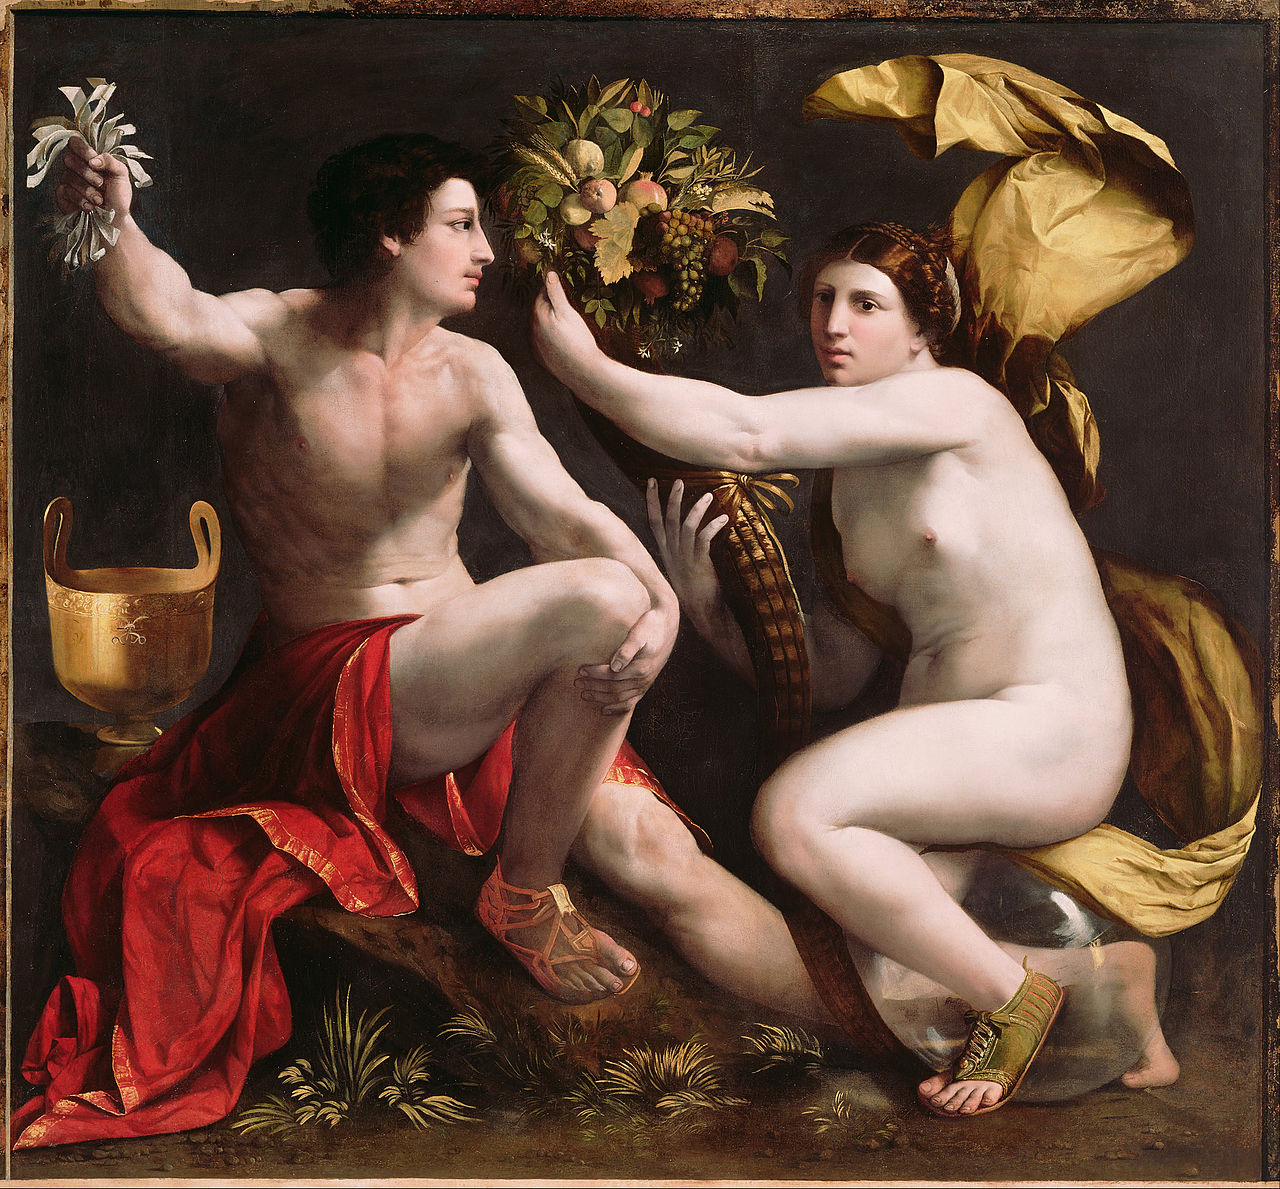
\includegraphics{img/Dosso_Dossi.png} \emph{The Allegory of Fortune} by
Dosso Dossi (1486-1542). Fortuna (``Lady Luck'') can bring good luck
(fruit), but good luck tends not to last (she's sitting on a bubble).
She might also bring bad luck (missing sandal). Chance (on the left) is
holding lottery tickets. Art critics say Dosso Dossi believed life is a
lottery for everyone.
\end{marginfigure}

Lots of decisions are in between the extremes of known risk and unknown risk (ignorance). That is, we have some information so that we're not completely ignorant, but we don't have so much information that we can carefully and explicitly assign probabilities. Some presentations make a clear delineation between risk and ignorance, and will sometimes call the latter cases of uncertainty. Here we're going to use \emph{decisions under uncertainty} as an umbrella for the whole continuum that goes from risk to ignorance.

\hypertarget{practical-and-theoretical-problems}{%
\section{Practical and Theoretical Problems}\label{practical-and-theoretical-problems}}

One of the riches of studying decision-making is that the same conceptual tools can be applied to both practical and theoretical problems. Practical problems range from ones we experience in everyday life to the kinds we see on game shows. Theoretical problems are ones that no human is expected to actually face, but by thinking about how someone in such a theoretical situation would solve the problem we can better understand how to approach practical situations.

\begin{marginfigure}

\includegraphics{img/lets_make_a_deal.png} Monty Hall was creator and
host of the 1960's game show \emph{Let's Make a Deal}, which was
rebooted with Wayne Brady (not pictured).
\end{marginfigure}

\newthought{A famous practical decision problem} is \emph{The Monty Hall Problem} which is named after the host of the game show \emph{Let's Make a Deal}. On the show there are three doors, one of which with a prize behind it. You get to pick one of the doors. Let's say you pick A. The host now opens one of the other two door that you did not pick. But of course, the host doesn't want to give away the game, so the door they open will be empty. Let's say they opened B and sure enough it's empty. Now the host asks, do you want to switch your choice to door C or stick with your current choice of A? Take a moment to think what you would do.

Most people have the intuition that switching your choice makes no difference. That is, that both doors A and C have equal chances of having the prize: each is 50\%. That is even what many professors of statistics and mathematics find sensible. But the right answer is that you switch! After the host opens door B, you are twice as likely to win the prize if you switch your choice to C than you are sticking with your choice. The reasoning is subtle and we'll need to use concepts from probability theory, which we will get to soon enough. But to give you a feel, ask yourself: if instead of three doors there were 100 doors, and the host closed 98 of the doors, would you switch your choice then? Or imagine two people playing the game many times, one person that always stays with their choice, the other always switches. Who is expected to win more often in the long run?\footnote{You can try out these strategies for yourself \href{http://www.rossmanchance.com/applets/2021/montyhall/Monty.html}{HERE.}}

\newthought{A famous theoretical problem} is \emph{Newcomb's Problem}. Suppose you are on a game show and there are two boxes in front of you: A and B. The contents of box A are concealed, but box B is completely transparent. Inside of transparent box B is \$1000. The options you are given might seem a bit strange, but this is what they are: take the unknown contents of box A (this is called the 1 box option), or to take the contents of both box A and box B (this is the 2 box option). Here's the twist, and this is what makes this a theoretical problem. While the contents of box A are unknown to you, there is an extremely sophisticated artificial intelligence that is very good at predictions. We'll suppose this AI has made perfect predictions every time in the past. The game show host consults the AI and does the following. If the AI predicts that you will pick the 1 box option (i.e., you pick the unknown contents of A) then the host will put in \$1,000,000 in box A. If, on the other hand, the AI predicts that you will pick the 2 box option, then the host will leave box A empty. All of this was already done before you are presented with the options. We can use a decision matrix to represent the example:

\begin{longtable}[]{@{}lcc@{}}
\toprule
& AI predicts two box & AI predicts one box\tabularnewline
\midrule
\endhead
\textbf{One box (just A)} & \$0 & \$1,000,000\tabularnewline
\textbf{Two box (A and B)} & \$1,000 & \$1,001,000\tabularnewline
\bottomrule
\end{longtable}

Here's one way of reasoning about what to do. The fact is that there's either a million dollars in box A or there's not, your choice won't make the difference. If there is a million dollars in box A, then picking the two box option is better than the one box option. After all, \$1,001,000 is more than \$1,000,000. If box A is empty, then the two box option means that you'll get at least \$1,000, which is better than \$0. Either way, the two box option is better.

As compelling as that argument might be, here's another line of reasoning that gets us to the exact opposite conclusion. You know that the AI has an incredible track record. Of the hundreds of people on the game show before you, the AI has gotten all of the predictions correct: those who picked the one box option got one million dollars, and those who picked the two box option got one thousand dollars. You want to be like those in the first group and get a million dollars rather than those in the second. So, you should pick the one box option.

Which of these arguments is better?

Earlier I claimed that thinking about theoretical problems can help us approach practical situations. So, are there any applications of Newcomb's problem?

A central feature of Newcomb's problem is that there is something in the world that is tracking decision making processes that then leads back into a decision problem. In the fantastical case it was an AI making predictions. We can remove this fantastical part and think instead of examples where there is a common cause between the world being in a certain state and you making a choice. Let's look at a version of the example we started this chapter with.

One of the things that makes annoying guy so annoying is that he loves to talk about the projects he's working on, projects you just don't care about. Come to think of it, you realize that you are actually quite similar to annoying guy: You also like working on projects and talking about them. That's why your friends find both of you annoying, especially if both of you show up. They don't mind having just one of you there, though (they have just enough tolerance for one annoying person, say). We can set up a decision matrix that looks like this:

\begin{longtable}[]{@{}lcc@{}}
\toprule
& Annoying guy stays home & Annoying guy shows up\tabularnewline
\midrule
\endhead
\textbf{You stay home} & 2 & 0\tabularnewline
\textbf{You show up} & 3 & 1\tabularnewline
\bottomrule
\end{longtable}

If you knew that annoying guy stayed home, you'd prefer to show up (3 is better than 2). If annoying guy showed up, you'd still rather be playing in the park than be at home (1 is better than 0). That said, if you both stayed at home, that would be better than both showing up (2 is better than 1). So what should you do?

Here's one line of reasoning that resembles the argument for the two box option above. Either annoying guy is going to stay home or show up. If he stays home, you prefer to show up and play. If annoying guy shows up, you still prefer to show up. So whether annoying guy stays home or shows up, you prefer to show up. So you should decide to go.

What the above argument does not consider is that annoying guy is just like you. That means whatever you decide to do will be a good prediction of what annoying guy decides to do. In fact, we could suppose that his decision matrix is identical to yours, except that in his mind you are the annoying one. It may help to explicitly represent things from annoying guy's perspective by transposing the above table as follows.

\begin{longtable}[]{@{}ccc@{}}
\caption{\label{tab:unnamed-chunk-3}From the perspective of annoying guy, his table would look like this.}\tabularnewline
\toprule
e & You\_stay\_home & You\_show\_up\tabularnewline
\midrule
\endfirsthead
\toprule
e & You\_stay\_home & You\_show\_up\tabularnewline
\midrule
\endhead
He stays home & 2 & 3\tabularnewline
He shows up & 0 & 1\tabularnewline
\bottomrule
\end{longtable}

So here's an alternative line of argument. Because of how similar you two are, there's little chance that one of you will show up while the other doesn't. In other words, it's much more likely that you both choose the same thing and you both show up or you both stay home. You prefer the outcome of both staying home than both showing up (2 is better than 1). So, you should decide to stay home, and that's likely what annoying guy will choose to do as well (since he'll be reasoning similarly). Your friends couldn't be more pleased.

The key difference between these arguments is whether you are using information about the decision you are making in assessing the probabilities of the outcomes, or whether the probabilities of the outcomes are independent of your choice.

Later on we will see how these arguments can be made more precise. There will be two ways of specifying the probabilities of outcomes, one that does not conditionalize on choices, and one that does. In addition, we will see how the fact that this crossroad exists at all means that the two most popular principles of decision making can come apart even though they agree most of the time. One is called \emph{the dominance principle} and the other is called \emph{maximizing expected utility}. But let's not get too ahead of ourselves. First we'll turn to some decision making concepts that rely on what we have implicitly been assuming: that preferences form ordinal rankings.

\hypertarget{summary}{%
\section{Summary}\label{summary}}

The most basic model of a decision has the following four ingredients:

\begin{enumerate}
\def\labelenumi{\arabic{enumi}.}
\tightlist
\item
  At least two exclusive choices/options/actions, which we represent as rows in a table.
\item
  At least two states of the world (that are out of our control), which we represent as columns.
\item
  Outcomes, the cells in the table.
\item
  Preferences, the numbers we assign to the outcomes, where higher numbers represent outcomes we prefer relative to others.
\end{enumerate}

Rationality can be understood \emph{descriptively} and \emph{normatively}.

Some decisions are made under certainty, but most of the ones we'll study are under uncertainty.

Decision theory, as we'll study it, draws from both theoretical and practical considerations.

\hypertarget{exercises}{%
\section*{Exercises}\label{exercises}}
\addcontentsline{toc}{section}{Exercises}

\begin{enumerate}
\def\labelenumi{\arabic{enumi}.}
\item
  If there are two possible world states and three possible actions, how many possible outcomes are there?
\item
  What are the rows in a decision table?

  \begin{enumerate}
  \def\labelenumii{\alph{enumii}.}
  \tightlist
  \item
    Things that you can control in the decision
  \item
    Things that are outside of your control in the decision
  \item
    Things you wish you could contorl but you can't.
  \item
    The outcomes of your decision.
  \end{enumerate}
\item
  Suppose Dr.~Smith is conducting an experiment on whether people prefer one marshmallow today or two marshmallows tomorrow. Which of the following best describes the field that Dr.~Smith's experiment is contributing to?

  \begin{enumerate}
  \def\labelenumii{\alph{enumii}.}
  \tightlist
  \item
    Descriptive decision theory, because Dr.~Smith is getting information about how many people choose the correct option: one marshmallow today.
  \item
    Normative decision theory, because Dr.~Smith is using normative claims and testing which ones are true.
  \item
    Descriptive decision theory, because Dr.~Smith is collecting information about how people make a choice between present and future outcomes.
  \item
    Normative decision theory, because there is no correct answer.
  \end{enumerate}
\item
  Normative decision theory aims to describe\ldots{}

  \begin{enumerate}
  \def\labelenumii{\alph{enumii}.}
  \tightlist
  \item
    how things are.
  \item
    how things ought to be.
  \item
    how decisions ought to be made.
  \item
    how decisions are made.
  \end{enumerate}
\item
  You're at the Kentucky Derby deciding on whether to bet on this year's favorite horse: The Decider. The probability of The Decider winning is 1/7. Which of the following describes the kind of decision you're considering and why?

  \begin{enumerate}
  \def\labelenumii{\alph{enumii}.}
  \tightlist
  \item
    Decision under known risk, since there is a body of evidence, like past races, that supports the claim that the probability that The Decider will win is 1/7.
  \item
    Decision under unknown risk, since nobody can be certain that The Decider will win.
  \item
    Decision under certainty, since we know that the chances of The Decider winning is 1/7.
  \item
    Decision under unknown risk, since there is a larger body of good evidence that the other horses haven't done very well when racing against The Decider.
  \end{enumerate}
\item
  In various forms of gambling like roulette or poker, one can assign probabilities to the outcomes and make a prediction accordingly. This is known as a\ldots{}

  \begin{enumerate}
  \def\labelenumii{\alph{enumii}.}
  \tightlist
  \item
    Decision under risk
  \item
    Decision under uncertainty
  \item
    Decision under ignorance
  \item
    Decision under the influence
  \end{enumerate}
\item
  You're at a small funeral with people you know very well. You, like everyone else, knows for certain that death is coming for us all, but we are uncertain about when that day will be. You're deciding between three options: i) say some kind words about the deceased, ii) say some honest but unkind words about the deceased, and iii) say nothing at all. What kind of decision scenario is this most like?

  \begin{enumerate}
  \def\labelenumii{\alph{enumii}.}
  \tightlist
  \item
    Decision under deceased influence.
  \item
    Decision under certainty.
  \item
    Decision under ignorance.
  \item
    Decision under risk.
  \end{enumerate}
\item
  Suppose you are on a game show where they have the same setup as Newcomb's problem. The host has already consulted with the devil and chosen to either put the money in Box A or not. Just as you are about to make your choice between the one box and two box option, you happen to get a trustworthy glimpse of the contents of Box A, which turns out to be empty. What option do you pick?

  \begin{enumerate}
  \def\labelenumii{\alph{enumii}.}
  \tightlist
  \item
    Two-box option
  \item
    One-box option
  \end{enumerate}
\item
  Suppose you are on a game show where they have the same setup as Newcomb's problem. The host has already consulted with the devil and chosen to either put the money in Box A or not. Just as you are about to make your choice between the one box and two box option, you happen to get a trustworthy glimpse of the contents of Box A, which turns out to \textbf{have \$1 million}. What option do you pick?

  \begin{enumerate}
  \def\labelenumii{\alph{enumii}.}
  \tightlist
  \item
    Two-box option
  \item
    One-box option
  \end{enumerate}
\item
  True or false: in the Monty Hall problem, it's essential to the puzzle that the host doesn't want to expose the prize. If they didn't care about giving away the location of the prize, there would be no reason to switch when they open door C.\footnote{This question comes from \emph{Chapter 1} of Jonathan Weisberg's \emph{Odds and Ends}.}
\item
  A characteristic feature of game theory is what?

  \begin{enumerate}
  \def\labelenumii{\alph{enumii}.}
  \tightlist
  \item
    The rows are options that both you and someone else jointly control.
  \item
    The world states are the actions of someone else.
  \item
    It is decision theory applied in the domain intellectual games, including the solving of a Rubik's cube.
  \item
    Game theory is not a real thing. You made this up.
  \end{enumerate}
\end{enumerate}

\hypertarget{ranking}{%
\chapter{Ranking}\label{ranking}}

This chapter will be on decision making that relies primarily on ranking outcomes. So far we have been using numbers to represent how much we like an outcome, where higher numbers represent outcomes we prefer more than outcomes with lower numbers. More specifically, we have been using what are called \emph{ordinal utilities}\footnote{\textbf{Ordinal utilities} make qualitative comparisons (x is better/same than y) but not quantitative comparisons.} where all we care about is whether one outcome is better, the same, or worse than another outcome. That is, we aren't paying attention to how much more we prefer one outcome to another. We'll get to that later. For now, if there are four outcomes and we give the one we prefer the most a utility of 4, we could have also given it a utility of 400. All that matters for ordinal utilities is that they rank outcomes from best to worse (with possible ties).

To get a feel for what decision making rules look like, we'll start with some simple ones. Because of their simplicity, they may not seem like very plausible rules and so we won't ultimately suggest that these should be followed. But understanding what the simpler rules get wrong is informative and will help us get a better idea for who to develop more sophisticated decision making rules.

\hypertarget{maximin-and-maximax}{%
\section{Maximin and Maximax}\label{maximin-and-maximax}}

Suppose you're a student that wants to have it all: you like going to parties, but you also take your studies seriously. Tomorrow there will be an exam, but you don't know if the professor has designed a difficult exam or an easy one. If you knew that tomorrow's exam were going to be an easy one, you'd prefer to go party, but if you knew that the exam were going to be a difficult one, you'd prefer to study and be prepared for it. And ``all things being equal'' between partying and studying, you have a preference to study because you can't stand the thought of getting a C grade - which is a possibility if the exam is a difficult one and you didn't study. Your preference assignment (pun intended) might look like this:

\begin{longtable}[]{@{}lcc@{}}
\toprule
& Difficult Exam & Easy Exam\tabularnewline
\midrule
\endhead
\textbf{Party!} & 1 & 3\tabularnewline
\textbf{Study!} & 4 & 2\tabularnewline
\bottomrule
\end{longtable}

What should you do?

Here's one decision rule you might use: Maximax. Maximax is a rule that says you should \textbf{max}imize the \textbf{max}imum outcome. The maximum utility in the above table is 4 and is assigned to the outcome in which you study and the exams turns out to be difficult. Of course, you can't control whether the exam will be a difficult one or an easy one (that's up to the professor), but Maximax doesn't really care. It just says you should pick the action that has the outcome with the highest utility.

Maximax isn't a very plausible rule if you care at all about risk. It has you choose outcomes with the highest payoffs, but with complete disregard for any possible outcomes with lower utilities. At a horse race Maximax says to bet on the drunk horse that's missing a leg because the payoff would be so much bigger than any of the other horses that clearly will leave the drunk one in the dust. Yes, it's possible that all the other horses suddenly have heart attacks at the start, but that possibility is so remote that you would be right to ignore it. At the very least, we should be incorporating information about the chances that the drunken horse will win, which are very, very low. Maximax doesn't do that. All that matters to Maximax is the size of the payoff. Nothing else.

Maximin is a much better rule. Maximin says to choose the least bad worst case scenario, i.e., \textbf{max}imize the \textbf{min}imum outcome. What you do is find the worst case scenario for each option, and then select the option with the least worst case. In the table above, the worst case scenario for the Party! option is 1 and for Study it is 2. Since 2 is greater than 1, Maximin says to study.

So far Maximax and Maximin agree, but they won't always. For example, suppose that your preference assignment is captured by the following table:

\begin{longtable}[]{@{}lcc@{}}
\toprule
& Difficult Exam & Easy Exam\tabularnewline
\midrule
\endhead
\textbf{Party!} & 1 & 4\tabularnewline
\textbf{Study!} & 3 & 2\tabularnewline
\bottomrule
\end{longtable}

Now Maximax and Maximin disagree. Maximax says to party, since it has the outcome with the highest utility (4). Maximin, on the other hand, says to study. Why? The worst outcome if you choose to party is 1, while the worst outcome if you choose to study is 2. Between those two, 2 is better than 1, and that can only happen in the choice to study.

Maximin is a pretty good rule if you are risk averse, that is, if you are predominantly worried about decreasing negative consequences.\footnote{The study of risk aversion is very rich and we'll return to this topic numerous times.} Not everyone may be as concerned about risk aversion as others. There are at least two ways of thinking about this. One is to understand differences between people's decision making as differences in the rules or strategies they use to make a choice. Another way to understand differences between people is to recognize differences in people's preferences. For example, if you're of the mindset that ``C's get degrees'' and you really love to party, then you might set up your preferences like this:

\begin{longtable}[]{@{}lcc@{}}
\toprule
& Difficult Exam & Easy Exam\tabularnewline
\midrule
\endhead
\textbf{Party!} & 3 & 4\tabularnewline
\textbf{Study!} & 1 & 2\tabularnewline
\bottomrule
\end{longtable}

For someone with this preference assignment, both Maximax and Maximin recommend that they should party. So the difference between why someone studies and why someone else parties might be a difference in preferences, or it might be a difference in the decision rules they're using. We'll turn to this point more shortly.

Maximin isn't without its own limitations. It can't, for example, help us decide what to do in certain situations where there are ties between outcomes across different options. Suppose someone is indifferent between all outcomes except the one where they studied and the exam was difficult. They might have the following preference assignment:

\begin{longtable}[]{@{}lcc@{}}
\toprule
& Difficult Exam & Easy Exam\tabularnewline
\midrule
\endhead
\textbf{Party!} & 1 & 1\tabularnewline
\textbf{Study!} & 2 & 1\tabularnewline
\bottomrule
\end{longtable}

Maximin doesn't make a recommendation about what to do because there is a tie between the worst outcomes of the two options: the worst in each case is 1. And yet, you might have the intuition that someone with this preference assignment should choose to study. But the reason, you might think, is not because they should use the Maximin rule. Rather, it's something about the relative comparison between partying and studying across the different possible world states. If you have this intuition, you'll already have a feel for the next decision making rule we'll explore: \emph{dominance reasoning}.

\hypertarget{the-dominance-principle}{%
\section{The Dominance Principle}\label{the-dominance-principle}}

The dominance principle does a more sophisticated comparison between options. There are two versions, a \emph{weak} version and a \emph{strong} version.

Suppose there are two options, A and B. We say that option A \emph{weakly dominates} option B if, for every world state, A is at least as good in its outcome as B. In other words, what we do is this. We check every column to make sure that A is at least as good as B. If so, then A weakly dominates B. If not, then A does not weakly dominate B. Let's look at same table again:

\begin{longtable}[]{@{}lcc@{}}
\toprule
& Difficult Exam & Easy Exam\tabularnewline
\midrule
\endhead
\textbf{Party!} & 1 & 1\tabularnewline
\textbf{Study!} & 2 & 1\tabularnewline
\bottomrule
\end{longtable}

Under ``Difficult Exam'' the option to study is at least as good as partying (2 is better than 1) and under ``Easy Exam'' the option to study is also at least as good as partying (1 is the same as 1). So, by the definition of weak dominance we just gave, the choice of studying weakly dominates the choice to party. Notice that we are \emph{not} doing a comparison between options across two different states (e.g.~bottom left and top right), our comparisons are between options in the same column.

The Weak Dominance Principle says to \emph{never pick weakly dominated options}. In the above table, studying weakly dominates partying, or in other words, partying is weakly dominated by studying. So the Weak Dominance Principle recommends that you do \emph{not} party. Since there are only two choices in our example, by the process of elimination the only option you are left with is to study.

We say that option A \emph{strongly dominates} option B if in every state option A is \emph{strictly better} in its outcome than B. Notice that in the above table, while it is true that under Difficult Exam studying is strictly better than partying (2 is higher than 1), the same is not true under Easy Exam - here both options are equal. That means that studying does not strongly dominate partying. So, it is possible that an option can weakly dominate another, but not strongly dominate it.

But let's suppose that the preference assignment was just a little bit different for the outcomes under Easy Exam:

\begin{longtable}[]{@{}lcc@{}}
\toprule
& Difficult Exam & Easy Exam\tabularnewline
\midrule
\endhead
\textbf{Party!} & 1 & 3\tabularnewline
\textbf{Study!} & 2 & 4\tabularnewline
\bottomrule
\end{longtable}

Here the option to study both weakly dominates the option to party, and it strongly dominates it. In fact, whenever an option is strongly dominated by another option, it is also weakly dominated by it.

The Strong Dominance Principle says to \emph{never pick strongly dominated options}. In the table just above partying is strongly dominated by studying (which means partying is also weakly dominated by it), so the Strong Dominance Principle says to not pick the option to party. Here both the strong and weak versions of the Dominance Principle agree.

Notice again that it doesn't matter that the best outcome for partying (3) is better than the worst outcome for studying (2). The two options are being compared column by column (i.e.~state by state). Notice also that the Dominance Principle, or ``dominance reasoning'', agrees with the recommendations of Maximin and even Maximax.

\hypertarget{more-than-two-options-and-two-states}{%
\section{More than two options and two states}\label{more-than-two-options-and-two-states}}

The decision making rules we've explored so far can be generalized to situations where there are more than two options. It can be helpful here to think a bit more abstractly. Let's say there are three options, A, B, and C. And suppose there are two world states, 1 and 2. Then we need a table with three rows and two columns. Finally, let's fill in the outcomes with the following utilities:

\begin{longtable}[]{@{}lcc@{}}
\toprule
& World State 1 & World State 2\tabularnewline
\midrule
\endhead
\textbf{Option A} & 2 & 4\tabularnewline
\textbf{Option B} & 1 & 3\tabularnewline
\textbf{Option C} & 5 & 6\tabularnewline
\bottomrule
\end{longtable}

Here it becomes apparent why we stated the Dominance Principle the way we did. We said to \emph{never pick dominated options}. Notice we didn't say ``pick an option that dominates another option''. This is because it is possible for an option to dominate another, but be itself dominated by some third option. By saying ``never pick dominated options'' we ensure that the option is not bested by some other one. So while in the example above it's true that A dominates B, it is also true that A is dominated by C (i.e., C dominates A). Option C, however, is not dominated by any other option. In fact, it's the only option that isn't dominated by another, and hence that is what dominance reasoning recommends.\footnote{You should make sure you can do this reasoning on your own. It's helpful to focus on just two options at a time, and then striking one out if it is dominated.}

Notice that in this example all of our decision rules so far agree: they all recommend Option C. But the \emph{reason} for their recommendations are all different. For Maximax it is because C has the outcome with the highest utility of 6. For Maximin it is because C has the least worst outcome with a utility of 5. And for Dominance Reasoning it is because it is the only option that is not dominated by any other. We will leave it as an exercise to ponder whether these reasons can ever make different recommendations.

You may also notice that none of the rules we've used are limited to decisions that have only two world states. This is most obvious in the case for Maximax: just look for the outcome with highest utility, follow that row to the left, and then pick the option that corresponds to that row. For Maximin you look for the lowest utility in each row, and then pick the option that has the highest one of these. Dominance reasoning is a bit more complicated, but not by much. When there are two columns, you are comparing two options to see if one is dominated by another, and you do this by checking the first column and then the second. In a decision matrix that has three columns you do the same thing, but you have to compare the two options in the additional third column. In other words, each additional world state means that you have to check an additional column when you're asking whether one option dominates another.

\hypertarget{non-unique-recommendations}{%
\section{Non-Unique Recommendations}\label{non-unique-recommendations}}

We mentioned earlier that there are at least two different explanations for why two different people might make different decisions, even if they have the same options and the same world states in their decision tables. One explanation is that they could be using different decision rules: maybe one person is using Maximax while another is using the Dominance Principle. We know that these rules can make different recommendations, so perhaps that explains the difference in two people's choices. (Question for reflection: can someone using the Dominance Principle come to a different recommendation than Maximin?)

Another possible explanation for differences in decisions is a deference in preferences. We've seen this already as we considered different preference assignments. For example, one student might have the mindset that ``C's get degrees'' and very much enjoy a good party. So they might have their preferences like this:

\begin{longtable}[]{@{}lcc@{}}
\toprule
& Difficult Exam & Easy Exam\tabularnewline
\midrule
\endhead
\textbf{Party!} & 3 & 4\tabularnewline
\textbf{Study!} & 1 & 2\tabularnewline
\bottomrule
\end{longtable}

A student with this above preference assignment will come to the conclusion that they should party, regardless whether they follow Maximax, Maximin, or the Dominance Principle.

Another student might have post-graduation ambitions that require higher grades than C. Moreover, they might not be fond of parties much anyway. So they might have a preference assignment like this:

\begin{longtable}[]{@{}lcc@{}}
\toprule
& Difficult Exam & Easy Exam\tabularnewline
\midrule
\endhead
\textbf{Party!} & 1 & 2\tabularnewline
\textbf{Study!} & 3 & 4\tabularnewline
\bottomrule
\end{longtable}

The student with this above preference assignment will come to the conclusion that they should study, regardless of whether they follow Maximax, Maximin, or the Dominance Principle.

In other words, the answer of what to do is not unique, even if two people agree on a decision rule. Different people could have different preferences, which can lead to different recommendations. So rationality, in so far as we have been considering dominance reasoning, does not demand that we all make the same choice. But be careful, that does not mean that we can choose anything we like without being irrational - we have to be mindful of what our aims or goals are. For example, while it may be rational for the first student to go party (after all, that's what dominance reasoning tells them to do), it would not be rational for the second student to go party. Our intuitive judgment suggests this is because going to the party is at odds with the goals of the more ambitious student. The dominance reasoning strategy gives us the same result given that the preference assignment in the second decision matrix reflects the aims of that student.\footnote{This is what we had in mind by \emph{instrumental} rationality.}

Notice that dominance reasoning proceeds by comparing options. We will see with other rules that there are alternative ways of making comparisons. But at the heart of most rules is the idea that options are assessed by how they are expected to perform relative to each other. We will see scenarios where this feature of decision making can get us into trouble and will try to find fixes for that.

It's important that you don't confuse the comparative nature of decision making with relativism. Relativism is a position about the nature of truth, particularly truths regarding ethical claims. While there are some connections between the normative aspects of decision theory and the study of morality, decision theory makes no commitments about the nature of truth. Well, almost none. We'll get to that later when we consider the nature of probability. But for now, make sure that you recognize that while we are working with the understanding of rationality in the instrumental sense (what should you do \emph{given} some goals or preferences) that is not the same as relativism.\footnote{Another helpful way of thinking about the difference is that instrumental rationality still makes room for critiquing decisions, while standard accounts of relativism rebuff judgment.}

\hypertarget{independence-of-options-and-states}{%
\section{Independence of Options and States}\label{independence-of-options-and-states}}

When we have been organizing our tables, we have been more or less assuming that the world states are ``out of our control'' while the options are the things that we can control by making a choice. That is, we have been assuming that options and world states are somehow independent of one another.\footnote{These notions of control and independence are central and we'll return to them again later.} This is a common assumption that is made in decision theory. An outcome (a cell in the table) is a combination of an action (a row) and something the world does (a column). When we insist that states and options are independent, then dominance reasoning seems pretty straight forward.

What if we weren't so strict about such independence? What if we don't ``factorize'' the outcomes into the two separate components of states and options? If we don't, then we may find that dominance reasoning isn't as straightfoward as we might think. Here is an example from Jim Joyce.\footnote{\emph{The Foundations of Causal Decision Theory}, pp115-6.} Imagine you park your car in a sketchy neighbourhood and someone promises to ``protect'' your windshield from harm. They offer their services for a mere \$10. You know that those who refuse this offer tend to find their windshield smashed, while those who take it don't. You also know it costs about \$400 to replace your windshield. We can represent this example of extortion with the following decision matrix, where we've put the utility number in front and the monetary cost in parentheses.

\begin{longtable}[]{@{}lcc@{}}
\toprule
& Broken Windshield & Unbroken Windshield\tabularnewline
\midrule
\endhead
\textbf{Pay Extortion} & 1 (-\$410) & 3 (-\$10)\tabularnewline
\textbf{Don't Pay} & 2 (-\$400) & 4 (\$0)\tabularnewline
\bottomrule
\end{longtable}

Let's use dominance reasoning. This means that to decide what to do, we check whether there is a unique option that is not dominated. When we look at the state of Broken Windshield, the Don't Pay option is better than Pay Extortion. When we look at the Unbroken Windshield state, we again see that Don't Pay is better than Pay Extortion. Because in each state Don't Pay is better than Pay Extortion, the Pay Extortion option is strongly dominated by Don't Pay. There are no other options and Don't Pay is not dominated by any other option. So according to dominance reasoning, you should not pay the extortion.

But wait. You know very well that if you don't pay the extortion then the most likely outcome is that you'll find yourself with a broken windshield. You're not really saving yourself \$10 at all, you're effectively guaranteeing that you'll have to pay \$400. Between the outcome of losing \$400 and paying \$10, you'd rather pay the extortion. And so, you reason, you should pay the extortion.

What's gone wrong? Dominance reasoning says you shouldn't pay the extortion money, but your own line of reasoning says you should. Is the dominance principle a bad rule after all?

Part of what's going on is how we've set up the decision matrix. While the matrix sets up an outcome for not paying and having an unbroken windshield, it's less clear that this outcome is the result of two independent components. In fact, there seems to be a causal relationship between the options and the states. The state of an unbroken windshield will depend in part on whether you choose to pay the extortion or not. What we want when we set up a decision matrix is the following: outcomes should depend on the combination of a state and a choice, but states and choices should not depend on each other.

Later we will see different ways of thinking about what it means for states and choices to be independent, and some of them will lead to different recommendations. For the time being, we will stick to clearer cases where states are independent of options. In these cases, dominance reasoning seems to align with our intuitive judgments of what to do.

Here's an example where worlds states are independent of options. Suppose your friends are trying to convince you to go camping this weekend. You're indifferent - you like staying home as much as you like being with your friends when camping. Except when it rains. You really hate camping in the rain and you'd much prefer to stay home. Here's a decision matrix set up for us.

\begin{longtable}[]{@{}lcc@{}}
\toprule
& Rain & No rain\tabularnewline
\midrule
\endhead
\textbf{Go camping} & 1 & 3\tabularnewline
\textbf{Stay home} & 2 & 3\tabularnewline
\bottomrule
\end{longtable}

Following dominance reasoning, you should stay home because that option weakly dominates the option to go camping. This setup follows the above guideline that states should be independent of your choice: whether you go camping or stay at home will not impact the weather.

Here's an example of how things can go wrong in our modeling of a decision if we don't pay attention to the guideline of keeping options and states independent. Suppose, as we have in many of our examples, that you've got an exam tomorrow and suppose you're deciding whether to go to a party (and thereby not study properly) or to study (and thereby not party properly). It may be tempting to set up the states into Pass Exam or Not Pass Exam:

\begin{longtable}[]{@{}lcc@{}}
\toprule
& Pass Exam & Don't Pass Exam\tabularnewline
\midrule
\endhead
\textbf{Party!} & 4 (pass and party!) & 2 (fail and party!)\tabularnewline
\textbf{Study!} & 3 (pass but no fun) & 1 (fail and no fun)\tabularnewline
\bottomrule
\end{longtable}

Under this poorly created setup, you might reason that you should go party, since for each state the option to party is better than to study and therefore strongly dominates the option to study. This setup, however, is poorly designed. There is a causal relationship between studying and passing the exam, which means the options and states are not independent in the above decision matrix. Again, when we set up what the states are, we should think of them as those things that are outside of our control, while the options are the things that we do control. Passing an exam is something that you have at least \emph{some} control over, so it cannot be a candidate as a state in a decision matrix.

We can rework the example like the way we started this chapter, by understanding that the level of difficulty of the exam is up to the professor, it is not in your control. Moreover, we supposed that you're uncertain about whether your professor will create a difficult exam or not. Your choice to study or not will have an impact on the outcomes in terms of the grade you can expect to receive, but your choices are independent of the states (what questions your professor chooses). By taking this kind of care in our setup, we then have the kind of table that we started out with and that we can apply our decision rules to. The only thing that's left missing in this table is the preference assignment, i.e.~the ordinal utility that you would give to each outcome to rank them from best to worst:

\begin{longtable}[]{@{}lcc@{}}
\toprule
& Difficult Exam & Easy Exam\tabularnewline
\midrule
\endhead
\textbf{Party!} & (C grade and party!) & (B grade and party!)\tabularnewline
\textbf{Study!} & (B grade and no fun) & (A grade and no fun)\tabularnewline
\bottomrule
\end{longtable}

\hypertarget{exercises-1}{%
\section*{Exercises}\label{exercises-1}}
\addcontentsline{toc}{section}{Exercises}

\begin{enumerate}
\def\labelenumi{\arabic{enumi}.}
\item
  Peter is considering two different lotteries. Lottery 1 costs \$20 to play and there's a one in a billion chance that he could win the \$1M prize. Lottery 2 costs \$10 to play and there's a one in hundred chance that he could win the \$10k prize. Suppose Peter chooses to play Lottery 1. Which of the following decision rules is Peter most likely using?

  \begin{enumerate}
  \def\labelenumii{\alph{enumii}.}
  \tightlist
  \item
    Maximax
  \item
    Maximin
  \item
    Dominance (weak)
  \item
    Dominance (strong)
  \end{enumerate}
\item
  Consider the following table where the world states (columns) are the levels of difficulty of an upcoming exam and the rows are the options you are considering on Thursday evening:

  \begin{longtable}[]{@{}clll@{}}
  \toprule
  / & Very Hard & Somewhat Hard & Easy Exam\tabularnewline
  \midrule
  \endhead
  \textbf{Party!} & 1 & 6 & 12\tabularnewline
  \textbf{Study!} & 10 & 5 & 6\tabularnewline
  \textbf{Call Family} & 3 & 4 & 5\tabularnewline
  \bottomrule
  \end{longtable}

  \begin{itemize}
  \tightlist
  \item
    What does the weak version of dominance recommend?
  \item
    What does the strong version of dominance recommend?
  \item
    What does maximax recommend?
  \item
    What does maximin recommend?
  \end{itemize}
\item
  Using tables like the ones in this chapter as a starting point, but changing around numbers, see if you can think of examples of the following:

  \begin{itemize}
  \tightlist
  \item
    Is there an example of a preference assignment where Maximin and Dominance Reasoning make different recommendations? Why or why not?
  \item
    Is there an example of a preference assignment where Maximax and Dominance Reasoning make different recommendations? Why or why not?
  \end{itemize}
\item
  Think of a decision you've made in the past, say like whether to go to university or not. Make a table to represent such a decision, providing what you took to be the options and states. Then plug in numbers to rank the outcomes. Then apply the decision making strategies from this chapter. What recommendations do they make? Do they align with what you decided to do?
\item
  What kind of decision making strategy do you tend to use? Compare and contrast your strategy with the ones we've covered in this chapter.
\item
  One benefit of differentiating between different kinds of decision making strategies is that it can help us better understand other people's choices. Given the same decision matrix, two people could come to different conclusions of what do simply because of differences in their decision strategies. Think of an example of how the strategies in this chapter could lead two people to come to opposite recommendations, \emph{even if they agree on the same table}. Do some of these strategies have associations with psychological dispositions, like people you consider to be more introverted vs more extroverted?
\end{enumerate}

\hypertarget{transitivity-and-completeness}{%
\chapter{Transitivity and Completeness}\label{transitivity-and-completeness}}

So far we have been using \emph{ordinal utilities} to represent preferences, without having said much about exactly what utilities are other than we can rank them from best to worst (with possible ties). There are different accounts of what preferences are, and we'll get to some details later. All accounts of preferences, however, seem to agree on some core axioms - ``obvious claims'' - that govern preferences. We'll cover two in this chapter that apply to ordinal utilities. Other axioms will require us to have covered the concept of probabilities and other notions of utilities in more detail, so we'll wait to introduce those axioms later.

The two axioms we cover here are known as \textbf{transitivity} and \textbf{completeness}. Let's use ice cream flavours to briefly illustrate these. Transitivity says that if I prefer strawberry to chocolate, and I prefer chocolate to vanilla, then I prefer strawberry to vanilla. Completeness says that either I prefer strawberry to chocolate, or I prefer chocolate to strawberry, or I'm indifferent between the two flavours. The same goes when comparing these to vanilla.

Transitivity and completeness play important roles in thinking about what preferences are, particularly in the context of using ordinal utilities to rank things. In fact, they apply not only to the case of individuals making decisions, but also in thinking about how to aggregate preferences of individuals into a collective group preference. There are several ways of doing that aggregation, like voting, but we might think that some are better than others depending on how well they reflect the preferences of individuals.

The thought is, preferences are or should be transitive and complete, regardless of whether those preferences belong to an individual or to a group. The very rough reason is that decision making seems to require putting options into some kind of ordering (with possible ties), and any ordering will satisfy both the transivity and completeness axioms. The tools we have been developing won't work without being able to order things. But as we'll see, there are independent arguments for transitivity and completeness that go beyond the convenience they provide for being able to use our decision theory tools.

\hypertarget{notation}{%
\section{Notation}\label{notation}}

It will help to have some notation to express transitivity and completeness more succinctly. Let's say that `\(a\succ b\)' means that \(a\) is wanted more than, or preferred to, \(b\).\footnote{The symbol `\(\succ\)' is just like \(>\) except it applies to preferences between objects or outcomes, whereas \(>\) applies to the magnitude of two quantities. But for both symbols, imagine they are mouths about to eat the preferred things.} If instead we want to say that \(b\) is preferred to \(a\), then we would write `\(b\succ a\)'. If we want to express indifference between the two, because you'd be equally happy (or sad) with one or the other, then we'll say `\(a\sim b\)' or `\(b\sim a\)'. In some cases we'll want to say that `\(a\) is at least as good as \(b\)' and we'll use the notation `\(a\succeq b\)'.\footnote{You can read this as `\(a\) is strictly preferred to or equally as good as \(b\)'.}

Here are the two axioms using this notation, using \(x,y,z\) as variables for outcomes (or objects).

\begin{description}
\item[Transitivity]
If \(x\succ y\) and \(y\succ z\), then \(x\succ z\).
\item[Completeness]
Either \(x\succ y\) or \(y\succ x\) or \(x\sim y\).
\end{description}

Notice that the axioms are stated in a way that leaves them ambiguous to descriptive and normative interpretations. If the decision theory we're doing is descriptive, then these axioms describe real decision makers. If the decision theory is normative, then these axioms describe ideal decision makers - how people \emph{ought} to approach decisions.

In the descriptive case, the transitivity axiom is false if John prefers strawberry to chocolate and chocolate to vanilla, but prefers vanilla to strawberry. In the normative case, we would say that John is not being rational.

If John claims that he neither prefers strawberry over vanilla, nor vice versa, and moreover that he's also not indifferent to them, then the completeness axiom is false under the descriptive interpretation. In other words, completeness is false if strawberry and vanilla cannot be compared. Under the normative reading, John is failing to be rational: surely he's at least indifferent to either flavour if he doesn't prefer one over the other!

This last point almost sounds like an argument for why we expect people to have preferences that obey completeness - normatively, and perhaps descriptively too. The arguments that we're going to look at are typically used for the normative interpretation of the axioms. We'll look at arguments for or against each axiom in more detail in the following sections. But first, we need to understand a particular kind of conceptual tool that is used in these arguments.

\hypertarget{money-pump-arguments-for-axioms}{%
\section{Money Pump Arguments for Axioms}\label{money-pump-arguments-for-axioms}}

We might dig in our heels and insist that the whole point of calling the above principles `axioms' is that they do not require justification. Most decision theorists, however, think we can do better than that, i.e., we can provide arguments that justify the axioms.

Arguments for preference axioms tend to be pragmatic ones. Pragmatic arguments show that if someone violates an axiom, then they are guaranteed to lose in a decision problem - a decision problem that `rational' agents would not accept. One of the most famous pragmatic arguments is known as the \emph{Dutchbook Argument} which we'll get to when we cover the axioms of probability theory. When it comes to axioms of preference, the type of argument we'll see is known as a \textbf{Money Pump Argument}.\footnote{Some think that pragmatic arguments are a weakness and it would be preferable to justify axioms and other principles in some purely theoretical way. Others think that pragmatic arguments are actually a strength of the theory because it connects it to practice and actions.}

Here's an example of a money pump argument. Suppose, contrary to our definition, that \(a\succ b\) and \(b\succ a\), which is like saying that John prefers strawberry to vanilla, and also prefers vanilla to strawberry. If you're scratching your head as to how that's even possible, good. That means you're getting the feeling of this very odd scenario, and we're going to turn that tension into an argument. Suppose that John has some strawberry ice cream and you have some vanilla ice cream. Since John prefers strawberry to vanilla, you offer John one cent to trade. John accepts. In fact this is a good deal for him since the one cent cost is negligible. Now that John has the vanilla and you have the strawberry, you again offer John to trade for one cent. John should again accept, since he also prefers vanilla to strawberry. Since John's preferences are such that \(a\succ b\) and \(b\succ a\), you can `pump money' out of John over and over again by cycling back and forth between his preferences. The pragmatic argument now says that this is absurd. Surely even John should recognize his failure and give up at least one of the two preferences.\footnote{TODO: Make and insert a diagram.}

The strategy behind money pump arguments is to build a sequence of trades where the agent accepts each one, but by the end of the sequence of trades they are right back where they started, except with less money. In John's case, he started with strawberry ice cream, made two trades, ending up where he started (with strawberry) but with two cents less.

\hypertarget{arguments-for-transitivity}{%
\section{Arguments for Transitivity}\label{arguments-for-transitivity}}

It's important to recognize that not all relations are transitive. `Birth mother' is not transitive: If Sally is the birth mother of Laura, and Laura is the birth mother of Jill, it is not the case that Sally is the birth mother of Jill. Another example of a non-transitive relation is `\(x\) is a better team than \(y\)'. It is not uncommon that team A wins a game against team B, that team B wins against team C, but also that C wins against A. On the other hand, `is taller than' is transitive: if John is taller than Bob, and Bob is taller than Paul, then John is taller than Paul.

Decision theorists claim that preferences are transitive. That is, whenever there are two preferences, \(x\succ y\) and \(y\succ z\), then there is a third, \(x\succ z\). If preferences are transitive, then it serves as a reason for avoiding the following money pump decision scenario.

Let's say, contrary to the transitivity axiom, that John's ice cream preferences are such that S\(\succ\)C, C\(\succ\)V, and V\(\succ\)S (where `S', `C', and `V' stand for strawberry, chocolate, and vanilla, respectively). We're going to set up a sequence of trades that John should accept, but land him in the same starting position, except with less money. Say John starts with chocolate. Then since S\(\succ\)C, he'll accept a trade for strawberry for a very small price, say one cent. Now with strawberry in hand, John would also accept a trade for vanilla, especially if this trade is free. Finally, John should also accept a trade back for chocolate, especially if, again, it's free. Now John is back in the original starting place (with chocolate), except with one cent less. We could also have charged John a small for the other two trades, or for any one of them - it doesn't matter so long as some cost, no matter how small, is charged somewhere along the way. Since the sequence of trades takes us back to the same starting condition, we can repeat the sequence again, and thereby `pump' money out of John indefinitely.\footnote{TODO Make and insert a diagram.}

Compare Sally to John. She also holds that S \(\succ\) C and C\(\succ\)V, but contrary to John, her preferences are consistent with the transitivity axiom and she holds that S\(\succ\)V. So, like John, she would accept a trade for chocolate if she had vanilla, and she would also accept a trade for strawberry if she had chocolate. But unlike John, she would not trade for vanilla if she had strawberry, because that is the opposite of her preferences given that they are transitive. Sally thereby avoids the money pump scenario. Because Sally's preferences are transitive, she breaks the cycle that John cannot.

The transitivity axiom for decision theory claims that preferences are transitive. What it says is that some ordering of preferences are to be excluded, namely those that are not transitive. It is this ability to exclude non-transitive preference orderings that provides a reason for avoiding the type of money-pump scenario just described. A non-transitive preference ordering either has no reason for avoiding the scenario (which seems bad) or at the very least has the burden to provide some other reason. A person like John might foresee how they're going to be money pumped and decide not to accept any more trades. But that alone seems like a poor reason, since it acknowledges the badness of the consequences of non-transitive preferences, without suggesting an alternative. The burden falls on them to provide an explanation of how they can avoid being money pumped. That's why money pump arguments are pragmatic - it is a kind of burden shift, rather than a proof that no other reason exists.

\hypertarget{arguments-for-completeness}{%
\section{Arguments for Completeness}\label{arguments-for-completeness}}

Our ice cream example makes completeness seem almost trivial: either strawberry is preferred to chocolate, or chocolate is preferred to strawberry, or one is indifferent between the two. But the completeness axiom doesn't just hold for ice cream flavours, it holds for all objects and options that we can have preferences over.

It is often said that you can't put a price on a human life. In our way of putting it, that means for any given dollar amount \(x\) and for any life \(l\), it is neither the case that \(x\succ l\), nor \(l\succ x\), nor \(x\sim l\). This claim is saying that money and lives are not comparable. That is, they are \emph{incommensurable}.\footnote{Arguably there are word meanings that are incommensurable across languages. For example, some have argued that there is no translation in English of the German word `Weltanschauung'.}

The completeness axiom says that you \emph{can} compare money and lives. We might not like it, but the completeness axiom says it can be done. If government decision making is any indication, the completeness axiom is probably correct, though no politician would probably admit it. Here's a brief reason to think that governments do, at least implicitly, compare lives and money. If a citizen is lost at sea, for example, we may be willing to pay out a lot of money to organize a search and rescue party. Surely, however, there is a limit to how much money we would be willing to put up. Maybe we'd pay a million, or even more, but surely there is an upper bound, some value where, though it pains us deeply to have to admit it, the life is not worth the inordinate cost. While this example may be extreme, more route examples abound. Decreasing speed limits on highways would save lives, but people save time by driving faster, and that time can be used for work or leisure - and either way we can put a dollar amount on that. So the decision of where to set a speed limit is implicitly comparing lives to other things, like time and money.

Examples aside, there is a money pump argument for the completeness axiom. Not everyone finds it as compelling as the money pump argument for transitivity, but nevertheless, here it is. Suppose there are two objects, \(x\) and \(y\) that are said to be incommensurable. In addition, suppose that \(y^+\) is just like \(y\) but is strictly preferred to it.\footnote{Think of + like a small bonus.} Because \(y^+ \succ y\), a small cost would be acceptable to trade \(y\) in order to get \(y^+\). If we accept that it is permissible to swap incommensurable objects, then the money pump argument is up and running: start with \(x\), swap for \(y\), now pay to get \(y^+\), then swap back for \(x\), which is where we started.\footnote{TODO Make and insert diagram}

This money pump argument isn't quite as compelling because it relies on the assumption that incommensurable objects can be swapped. One might try to argue that incommensurability is supposed to be conceptually distinct from indifference. If we are indifferent between two objects, then it seems perfectly fine to swap between them. But the main thrust of saying that two objects are incommensurable is to say that is not straightforwardly permissible to swap (note this is not quite the same thing as saying that it is impermissible).

Putting aside the question about the conceptual difference between incommensurability and indifference, we can ask how it might show up in behavior. When you make a choice, we take this to ``reveal'' or provide evidence of your preferences. For example, suppose a subject is presented with objects \(a\) and \(b\), and they choose \(a\). This is evidence that they prefer \(a\) over \(b\), i.e., \(a\succ b\). (I'm cheating here by letting \(a\) and \(b\) refer to both the objects and the corresponding options, but not much is to be gained by being pedantic.) Of course mitigating circumstances might explain why they chose \(a\) even though they prefer \(b\): perhaps \(a\) would give them an opportunity to still choose \(b\) later (but not vice versa), or they were threatened (unbeknown to us) or something else. So it is a tricky business to infer preferences from choices that people make, but in some idealized circumstances, there is at least a rough inference we can make that goes from behavior to preference (more on this when we analyze utilities in more detail). How could we ever tell the difference, however, between incommensurability and indifference? The objection, from this perspective, is that any behavioral test for incommensurability can also be used for detecting indifference. We might for example, observe that sometimes \(a\) is chosen - in which case we would say that \(a\) is at least as good as \(b\) (\(a\succeq b\)) - and other times \(b\) is chosen - in which case \(b\) is at least as good as \(a\) (\(b\succeq a\)). Since each object is at least as good as the other, we are invited to infer \(a \sim b\). It is unclear how to design a behavioral test that would detect incommensurability without inviting the inference to indifference.

Another way to handle the possibility that some objects are incommensurable could be to restrict the domain of decision theory. If some objects are incommensurable, then those aren't the kinds of things we can have preferences over, and the theory can't make decisions about those things. This response somewhat captures the difficulty raised by the claim that, e.g., you can't put a dollar amount on a human life. One can understand this sentiment as trying to express that we can't, or ought not to be engaging in decisions when these objects are being considered.\footnote{But as we suggested above, we may not like it and may not want to make it explicit, but we do make implicit comparisons between money and life.}

The issues we've raised about completeness assume that comparisons must be done on a single scale. One strategy for handling these difficulties is to allow for different scales and then find ways of comparing the scales. This is known as the multi-attribute approach. However, to understand this approach requires a more sophisticated understanding of what sorts of things utilities are, and we'll cover that in a following chapter.

For now, we're going to look at other applications of decision making when we assume that preferences are transitive and complete. More specifically, we'll look at how groups can make decisions given preferences of individuals.

\hypertarget{social-choice}{%
\section{Social Choice}\label{social-choice}}

\hypertarget{group-decisions-are-not-mere-sets-of-individual-decisions}{%
\subsection{Group decisions are not mere sets of individual decisions}\label{group-decisions-are-not-mere-sets-of-individual-decisions}}

Almost all of the examples we have covered have been about individual choices. In many cases, however, it is not an individual that makes a choice, but a group of individuals. This leads to a separate set of questions about how groups do/should make choices. At the very least, the way a group makes a choice should in some way reflect the preferences of the individuals. It would be extremely odd if everyone unanimously agreed that the best option for the group is A, but then some other option is picked ``by the group'' that is unanimously agreed on to be the worst option.

That said, we will see that there are different ways in which we can be explicit about how a group (a collective of indivbiduals) should be connected to the preferences of the individuals that make up the collective. Social choice theory is about how to aggregate preferences of individuals into a single collective preference. It turns out that there are many ways of doing this aggregation. However, there can be tensions between the individual level and the collective level, particularly concerning the notion of rationality.

Here's a brief illustration of how such a tension could come about. Suppose that there are three judges, J1, J2, and J3. Each judge is ``rational'', which means at the very least that they subscribe to a rule of inference philosophers call \textbf{modus ponens} (a latin name for affirming the consequent). Modus ponens says that if you believe a conditional like `If A then B' is true and you also believe that `A' is true, then you should infer that `B' is true. For example, suppose you know that if Johnny eats peanuts then he will have an allergic reaction, and you also know that Johnny is eating peanuts, then you should infer that Johnny will have an allergic reaction!\footnote{Note that the other direction isn't valid, i.e., if you know that Johnny is having an allergic reaction, it's not guaranteed that that's because Johnny ate peanuts - he might have eaten something else that he's allergic to.}

Now suppose that each of our judges has been called on to make a decision about a case. The case is concerned about a purported incidence of theft of a water bottle. The judges are asked to assess the truth of the following three claims:

\textbf{S1} The defendent stole the water bottle.

\textbf{S2} If S1, then the defendant should go to jail.

\textbf{S3} The defendant should go to jail.

Each judge makes their own decision about the case, which are then collected in the table below.

\begin{longtable}[]{@{}cccc@{}}
\toprule
Judge & S1 & S2 & S3\tabularnewline
\midrule
\endhead
J1 & True & False & False\tabularnewline
J2 & False & True & False\tabularnewline
J3 & True & True & True\tabularnewline
\bottomrule
\end{longtable}

Notice that each judge meets the rationality constraint of obeying modus ponens: the only judge that says S3 (the defendant should go to jail) is the judge that also says S1 and S2 are true. In order to say that S3 is false, at least one of S1 or S2 would have to be false, and indeed that is consistent with what Judges J1 and J2 say.

In other words, each judge is individually rational. But what about the collective? For example, what if we aggregate the judgments of the judges and use the idea of majority to assign truth or falsity to the three statements? In other words, we might use \textbf{majority ruling} to aggregate the decisions into a group decision. If we do that, then we would have:

\begin{longtable}[]{@{}cccc@{}}
\toprule
Judge & S1 & S2 & S3\tabularnewline
\midrule
\endhead
J1 & True & False & False\tabularnewline
J2 & False & True & False\tabularnewline
J3 & True & True & True\tabularnewline
Group & True & True & False\tabularnewline
\bottomrule
\end{longtable}

Notice that the collective judgment \emph{violates} modus ponens, that is, it says that S1 and S2 are true, but S3 is false. Aggregating judgments by majority voting does not, in other words, preserve rationality from the individual level to the collective level.

Rationality is not the only thing that we might be concerned about when we aggregate things from the individual to the collective level. Not to mention, rationality is somewhat complex even at the individual level. So let's turn to something simpler.

What we'll focus on for the remainder of this chapter is whether there are ways to aggregate preferences in a consistently acceptable way. What counts as `'acceptable'' is something we'll discuss. To start, we'll look at some examples of how preferences might be aggregated, keeping track of advantages and disadvantages.

\hypertarget{plurality-and-runoffs}{%
\subsection{Plurality and Runoffs}\label{plurality-and-runoffs}}

One common form of aggregation, especially in elections in the United States, is plurality voting, also known as `first past the post' or `winner takes all'. Let's look at it in a simple context. Suppose there are seven people, P1, P2, \ldots{}, P7, that are long time friends and are deciding on where to go to dinner together. There are four restaurants they are considering, R1, R2, R3, and R4. Each person gets one vote. Suppose the table below summarizes the results of their vote.

\begin{longtable}[]{@{}lcccccccc@{}}
\toprule
& P1 & P2 & P3 & P4 & P5 & P6 & P7 & Total\tabularnewline
\midrule
\endhead
R1 & Yes & Yes & Yes & & & & & 3\tabularnewline
R2 & & & & Yes & Yes & & & 2\tabularnewline
R3 & & & & & & Yes & & 1\tabularnewline
R4 & & & & & & & Yes & 1\tabularnewline
\bottomrule
\end{longtable}

By these results, it looks like R1 should be the choice of the group, because it has the most `plurality' of votes.

Note, however, that while R1 has the most number of votes, it does not have the majority of votes. Suppose the P4-P7 are all strongly opposed to going to R1. Then an odd consequence of plurality voting is that that group goes to a restaurant that the majority of people in the group oppose.

One way to handle this is to have a `runoff' vote. If no option, such as an election candidate or restaurant (in our case), is the majority, then we hold a second vote between the top two vote getters. In our case that is R1 and R2. Suppose that such a second vote is held and we get the following results.

\begin{longtable}[]{@{}lcccccccc@{}}
\toprule
& P1 & P2 & P3 & P4 & P5 & P6 & P7 & Total\tabularnewline
\midrule
\endhead
R1 & Yes & Yes & Yes & & & & & 3\tabularnewline
R2 & & & & Yes & Yes & Yes & Yes & 4\tabularnewline
\bottomrule
\end{longtable}

In a runoff vote the recommendation we get for the group is to go to R2.

What plurality and runoff voting have in common is that they are aggregating people's first preferences. Little to no weight is given to people's second, third, or even last preferences.

This has some advantages. We saw above money pump arguments for thinking that individual preferences should be transitive and complete. One might like this to also be true of group preferences. So long as we restrict ourselves to the combination of plurality and runoff voting, the group preference will also be transitive and complete. But the reason for this is because the plurality+runoff system is ultimately just aggregating preferences for two options. Either there is an option that gets a majority of first preferences or not. If an option \(a\) gets a majority of first preferences, then \(a\) received at least one more than half the votes. Then for any other candidate \(x\), they can have at most one less than half the votes. So, \(a\) will be preferred to \(x\) and it's not possible to violate either transitivity or completeness. If an option \(a\) does not get a majority of first preferences, then it might be possible that \(a\) has more votes than another or less. But if \(a\) is one of the two options with the highest votes, then the runoff vote forces another vote between those to options, say \(a\) and \(b\). In this runoff vote, either \(a\) will get more than half, exactly half, or less than half of all the votes, which correspond respectively to the group preference being \(a\succ b\), \(a\sim b\), or \(b\succ a\). In each scenario, neither transitivity nor completeness are violated.

But a system that effectively ignores everything but people's ``first'' preference seems like an impoverished system. The consensus we get in the plurality+runoff system is forced. To see this, consider another system that takes into account other preferences besides the first. This is called the \emph{Borda count}.

\hypertarget{the-borda-count-and-an-impossible-task}{%
\subsection{The Borda Count and an Impossible Task}\label{the-borda-count-and-an-impossible-task}}

We'll illustrate the \textbf{Borda count} with our restaurant example. Let's suppose that each person ranks the restaurants, so that 4 points goes to the most preferred restaurant, 3 to the second, 2 to the third, and 1 to the least preferred. If we had five restaurants, we would have 5 points go the first, 4 to the second, etc. In general, if there are \(n\) restaurants, we give \(n\) points to the most preferred, \(n-1\) to the second, \(n-2\) to the third, etc. This method of aggregation is used in some college sports in ranking teams. Notice that it doesn't just take into account people's first preferences, but all preferences. Also notice that it does not capture how much more you might like one option over another. Again, all we are doing here is putting the outcomes in an order using ordinal utilities (an ordering that, at the individual level, will be transitive and complete).

Suppose we get the following results in our restaurant example.

\begin{longtable}[]{@{}lcccccccc@{}}
\toprule
& P1 & P2 & P3 & P4 & P5 & P6 & P7 & Total\tabularnewline
\midrule
\endhead
R1 & 4 & 4 & 4 & 1 & 1 & 1 & 1 & 16\tabularnewline
R2 & 1 & 3 & 3 & 4 & 4 & 2 & 2 & 19\tabularnewline
R3 & 3 & 2 & 2 & 3 & 3 & 4 & 3 & 20\tabularnewline
R4 & 2 & 1 & 2 & 2 & 2 & 3 & 4 & 15\tabularnewline
\bottomrule
\end{longtable}

Notice that the first preferences still align with our previous tables (all the 4's are in the `yes' positions). Also notice that R1 is still the least preferred for P4-7, which means we preserve the result we got from the runoff vote. However, unlike the recommendations of the plurality vote and the runoff vote, the Borda count recommends that the group go to restaurant R3.

So the Borda count has a nice feature in that it builds consensus by considering people's preferences beyond their first. Even though the group goes to a restaurant that is almost no one's first preference (in our example R3 does happen to be P6's most preferred), it finds a restaurant that is broadly acceptable in the group.

So far so good, but we might now ask: is the Borda count a way of aggregating individual preferences so that, if the individual preferences are transitive and complete, the group preference will be transitive and complete as well?

Let's look at the following example. It will help to organize our table a little differently so that we can tell just by looking what the vote tallies would be. Rather than put options in the rows, we'll organize the rows in terms of people's most to least preferred options, going from the top to the bottom. Let's say we have three people, P1, P2, and P3, and they are deciding between three books to read together next month: A, B, or C. The table below summarizes the three people's preferences from best (1st) to worst (3rd).

\begin{longtable}[]{@{}lccc@{}}
\toprule
Preference & P1 & P2 & P3\tabularnewline
\midrule
\endhead
1st & A & B & C\tabularnewline
2nd & B & C & A\tabularnewline
3rd & C & A & B\tabularnewline
\bottomrule
\end{longtable}

If we just compare the preferences between books A and B, then A would get 2 out of the 3 votes (whatever those points would be). If we just compare B and C, then B gets 2 out of 3 votes (2/3). So this might suggest that, in terms of the group preference, A is preferred to B and B is preferred to C. But when we inspect further and compare A and C, we'll see that C gets 2/3 votes. Our pairwise comparison produces a cyclical group preference: \(A\succ B\), \(B\succ C\), and \(C\succ A\). This is in violation of the constraints that group preferences should be transitive, i.e., if \(A\succ B\) and \(B\succ C\), then \(A\succ C\), not \(C\succ A\)!

One potential response to this cyclical situation is to say that the group should be indifferent to A, B, and C, i.e., \(A\sim B\sim C\). The problem with this suggestion is that we can't both accept it and the condition called \textbf{the independence of irrelevant alternatives} (or IIA). Suppose, for example, that book C is on back order and will not be delivered in time for the group to read next month. Book C is now an ``irrelevant alternative'' and we should drop it. But here is the problem. If we agreed that the group should be indifferent between the three groups, \(A\sim B\sim C\), then dropping \(C\), the irrelevant alternative, should not affect whatever preference holds between \(A\) and \(B\). That is, after dropping \(C\), the group should still be indifferent between \(A\) and \(B\), i.e.~\(A\sim B\). The preference between \(A\) and \(B\) is said to be \emph{independent} of the \emph{irrelevant alternative}. But let's look at the table again if we drop \(C\) there:

\begin{longtable}[]{@{}lccc@{}}
\toprule
Preference & P1 & P2 & P3\tabularnewline
\midrule
\endhead
1st & A & B & A\tabularnewline
2nd & B & A & B\tabularnewline
\bottomrule
\end{longtable}

The table makes it pretty clear that the group should prefer A to B. But maybe the group decides to hold themselves to their original agreement and uphold IIA. That is, since they had agreed that \(A\sim B\sim C\) before they knew that C was on back order, the group preference should still be \(A\sim B\) - despite what the new table says. The problem with this proposal is that it does not maintain the implicit fairness that each person's preferences gets equal weight in the group. To be indifferent between \(A\) and \(B\), the new table would have to assume that P2's preference for B is worth twice as much as P1's preference for A (and likewise P3's). That goes against the very point of aggregating their preferences through something like the Borda count. P2 would be something like a `'dictator'' in shaping the group preference.

Maybe another strategy is to leave behind the Borda count method entirely and instead require a consensus - a unanimous vote - in order for the group to prefer one option to another. If there is no consensus among the voters between two options, then the group shall be indifferent between those options. Looking at our tables, it is clear that there is no consensus that A is preferred to B, since P2 prefers B to A. This `method of consensus' is nice in that it satisfies IIA (independence of irrelevant alternatives) and does not give more weight to one person's vote over others. In fact, this `method of consensus' seems like the only possible solution to the `cyclical preferences' issue.

The problem with the consensus method suggestion, however, is that it violates transitivity. Suppose instead of the summary tables above, we had these results instead.

\begin{longtable}[]{@{}lccc@{}}
\toprule
Preference & P1 & P2 & P3\tabularnewline
\midrule
\endhead
1st & A & B & C\tabularnewline
2nd & B & C & A\tabularnewline
3rd & C & A & B\tabularnewline
\bottomrule
\end{longtable}

The group unanimously votes that A is preferred to C, and so by consensus we get \(A\succ C\). If we compare A and B, we notice that there is no consensus, and so by this method the group should be indifferent, i.e., \(A\sim B\). Similar inspection of the table means \(B\sim C\). Since we have \(A\sim B\) and \(B\sim C\), then by the transitivity constraint we should have \(A\sim C\), but our consensus method told us \(A\succ C\)!

The tension we are feeling is actually a very deep problem. It can be laid out explicitly in a formal argument and is known as \textbf{Arrow's Impossibility Theorem}. What it says, put intuitively, is that for any voting system that allows for three or more options, at least one of these three things will \emph{not} hold:

\begin{enumerate}
\def\labelenumi{\arabic{enumi}.}
\tightlist
\item
  Unanimity: If everyone prefers A to B, then the group prefers A to B.
\item
  Independence of Irrelevant Alternatives: If nobody changes their mind about the relative ordering of A and B, then the group can't change its mind about the relative ordering of A and B.
\item
  No Dictators: For each voter, it is possible that the group's ranking will be different to their ranking.
\end{enumerate}

To be clear, we are not saying that all voting systems are bad: some are worse than others. Presumably a voting system that satisfied none of these conditions is pretty unacceptable, especially in comparison to a voting system that at least satisfies No Dictators and Unanimity. What Arrow's Impossibility Theorem tells us is that it's impossible to have it all, i.e.~a voting system that obeys all three features.

\hypertarget{limitations-and-key-take-aways}{%
\section{Limitations and Key Take Aways}\label{limitations-and-key-take-aways}}

All that said, we have narrowed in on a result about group preferences that is deep, but not without a fair number of substantial background assumptions (some of which we have left implicit). For many group decisions, like friends choosing what restaurant to go to, some of the assumptions either might not hold, or the conditions don't impose a level of unfairness that we care too much about. For example, while we might have to allow one friend to dictate what restaurant to go to this Friday night, we might allow another friend to dictate where to go the following week. Or we might allow the group to split and go to do different restaurants (whereas in elections it is not typically possible to elect two presidents simultaneously). In any case, the range of Arrow's Impossibility Theorem is limited to several background assumptions, and while many political elections meet those assumptions and thereby face certain impossibilities, lots of group decisions don't meet those same background assumptions.

So we have seen the kinds of uses that ordinal utilities provide us with, particularly as a tool for ranking things, both on the individual and group level. They have also helped us introduce important concepts like transitivity and completeness, which we will make further use of in later chapters. But they have important limitations. Two are particularly relevant.

First, while ordinal utilities allow us to order outcomes from best to worst, they don't provide us with a way to say \emph{how much more} we might like one outcome over another. In our restaurant example, each person ordered or ranked their restaurants from most preferred to least preferred. But it possible that the difference between one person's first and second choice is very small, while for another person it is very large.

Second, ordinal utilities don't give us a way to compare how much one person's first choice is liked in comparison to another's: one person might absolutely love their first choice, while another person sees their first choice as bad, but the least bad among all the options. We'll see whether a different kind of numbering system that uses \emph{cardinal} utilities will help us with these two limitations. (Spoiler: they help for one, but not the other.)

\hypertarget{exercises-2}{%
\section*{Exercises}\label{exercises-2}}
\addcontentsline{toc}{section}{Exercises}

\begin{enumerate}
\def\labelenumi{\arabic{enumi}.}
\item
  Transitivity is a kind of pattern that some relations have. Intuitively, a relation can be anything that involves two objects. Examples include ``John is left of Sally'', ``this stone is heavier than this chair'', and ``Oliver is funnier than Connan''. It's helpful to think of transitivity in terms of a pattern that a relation R might have: if \(x\)R\(y\) and \(y\)R\(z\), then \(x\)R\(z\). Think of different kinds of relations you could plug into R and the kinds of objects that \(x\), \(y\), and \(z\) are related by R.

  \begin{itemize}
  \tightlist
  \item
    What are examples of relations that are transitive?
  \item
    What are examples of relations that are not transitive?
  \end{itemize}
\item
  Similarly to above, completeness is a kind of pattern that some relations have: either \(x\)R\(y\) or \(y\)R\(x\).

  \begin{itemize}
  \tightlist
  \item
    What are examples of relations that are complete?
  \item
    What are examples of relations that are not complete?
  \end{itemize}
\item
  \newthought{Money Pump Arguments.} Suppose you have two roommates named Peter and Sally. The three of you watch an episode from a series together every night of the week except Sundays. There are three different series that the three of you have been following together: Show A, Show B, and Show C. Because you own the device and pay for the streaming subscription, you get to pick which show to watch on any given night. Peter claims that he always prefers Show A over Show B, that he always prefers Show C over Show A, and that he always prefers Show B over Show C. Sally, on the other hand, is always indifferent between Show B and Show C, but she prefers Show A over either those two. Your preferences, however, change on a day to day basis, but you prefer not to watch the same show two days in a row and you want to see at least one episode from each show in any given week. That said, let's suppose that you'd be willing to let one of your roommates pick the show in exchange for one dollar. Explain how you could ``money pump'' one of these roommates but not the other. In your explanation, feel free to imagine that you'll make offers to Peter on every day for one week, and then to Sally on every day another week. What sequence of selections in a week would guarantee that you'll get \$6 from exactly one of those roommates?
\item
  Make a table like the Borda count restaurant example, but so that the group choice is not anyone's most preferred choice.
\item
  Make a table like the Borda count restaurant example, but so that the group choice is at least one person's least preferred choice.
\end{enumerate}

\hypertarget{utilities}{%
\chapter{Utilities}\label{utilities}}

There are three broad questions we would like to answer in this chapter.

\begin{enumerate}
\def\labelenumi{\arabic{enumi}.}
\item
  Is there a way for a person to represent \emph{how much more} one option is preferred to another?
\item
  Is there a way to compare one person's preferences to another that isn't just the ordering of the options? That is, can we say something more substantial about two people's first choice, like that one person likes it the most but another dislikes it the least?
\item
  How do we interpret what the numbers mean? What are the numbers referring to in the real world? That is, what is their content?
\end{enumerate}

\newthought{These questions are not just philosophical}. There are important practical considerations at stake. For example, the World Health Organization (WHO) has to somehow measure the value of medical interventions. The unit they use in their assessments is called a QALY - quality-adjusted life-year. A QALY incorporates both the quality and quantity of life lived. One QALY amounts to living one year in perfect health, while zero QALY amounts to death. The QALY is not without controversy and the debate ranges from purely philosophical considerations to the deeply pragmatic constraints that policy-makers face.\^{}{[}Another example that we will look at below is how the concept of utility can motivate arguments concerning social welfare and taxation.

We will introduce the idea of a \textbf{cardinal utility}.\footnote{Supposedly the first use of ``cardinal utility'' was in 1934 by John Hicks and Roy Allen.} The basic idea is to use what's called an \emph{interval} scale. In addition to being able to order things using numbers, the numbers are also meant to represent \emph{magnitudes}. Money is an example of an interval scale, to some approximation. We can use money not only to order things from most expensive to least expensive, but we can also say how much more expensive one thing is to another. One might think, however, that money is ultimately limited in how fine-grained it can be - perhaps it doesn't make much sense to speak of quantities that are smaller than a cent. Whether or not that's the case, cardinal utilities can be arbitrarily precise and are typically represented using real numbers (as opposed to whole numbers).\footnote{The ``real'' in ``real numbers'' doesn't mean something like ``actual numbers.'' The history of numbers and number systems is fascinating (see the Wikipedia entry for ``number''). The main thing for our purposes is just to know the difference between integer numbers and real numbers.}

\newthought{If we could build an interval scale for preferences}, we might be able to solve some of the limitations of ordinal utilities. For example, suppose there are four books, A, B, C, and D that both Alice and Bob are considering to read together next month. Using just ordinal utilities, it is easy enough for Alice and Bob to order the books with respect to their preferences: each will use 4 to represent their most preferred book, 3 the next preferred, and so on. But remember that we allow for ties, say between B and C. That is, it could be the case that both Alice and Bob agree in their preference orderings, so that \(A\succ B\sim C \succ D\). But what should we make of the situation where Alice assigns 4,3,3,1 for books A, B, C, D, respectively, while Bob on the other hand assigns 4,2,2,1 to them? These numbers preserve the same ordering, and so from an ordinal utility perspective they are the same, but Alice and Bob seem to want to say something different about how B and C compare to the extreme ends of their best and worst options. How do we even go about this?

\hypertarget{creating-an-interval-scale}{%
\section{Creating an Interval Scale}\label{creating-an-interval-scale}}

Here is one way to capture information about how much one option might be preferred to another. Suppose we have just three options and Alice orders them like this: \(A\succ B \succ C\). We want to find how much more Alice prefers B to C, and how much less she prefers B to A. To do so, we create a new option, L. We can think of option L like a lottery that will have A and C as ``prizes''. But what should the odds be of winning C in lottery L compared to the odds of winning A? Suppose lottery L has 100 tickets. Given that Alice prefers A over C, it seems that A should be on all of the tickets. But what we want to find out is how B compares to A and C. So what we do is figure out at what point Alice would be indifferent between B and L, where L specifies the fraction of all tickets where A wins and the fraction where C wins. Let's see some examples to illustrate.

Let's say lottery L has 50\% tickets with A and 50\% tickets with C. We ask Alice which of the preferences she has: \(B\succ L\), \(L\succ B\), or \(B\sim L\)? If Alice says \(B\succ L\), then this means that she prefers getting B to a 50\% chance of getting A. That is, she prefers B more than ``half as much'' as A. But that still doesn't tell us how much more than ``half as much'' as A. So, in this case we would change the lottery L to a new lottery L' by \emph{increasing} the fraction of tickets that would go to A and then ask for her preference again, comparing B to L'. If instead Alice had said \(L\succ B\), then that means that she prefers a 50\% chance of getting A than getting B. Here we would change the lottery L to a new lottery L' by \emph{decreasing} the fraction of tickets for A. Finally, if instead Alice had said \(B\sim L\), then that means she is indifferent between getting B and a 50\% of getting A. Here we wouldn't have to change anything about the lottery.

Suppose we have gone through this process and we find the lottery where Alice's preference between B and L is indifferent, i.e.~\(B\sim L\). And let's suppose that L has 75\% of the tickets go to A and 25\% to C. The idea behind creating an interval scale from this information is to think that Alice's desirability of B is 75\% of whatever her desirability of A is. For example, let's suppose that Alice's utility of A is 1 and her utility of C is 0. Then her utility of B would be 0.75. If instead Alice's utility scale were 0 to 8, with C at 0 and A at 8, then her utility of B would be 6.

INSERT ILLUSTRATION

So the introduction of a lottery option helps us make important progress on determining the magnitudes of utilities, but only \emph{relative} to the utilities of other options. That is, the lottery option procedure doesn't help us decide what the scale itself should be. It just helps us assign utilities given that we have some scale. To some extent this is a nice feature. Notice that, no matter what scale you pick, the lottery option procedure will always preserve the ordering given by the ordinal utilities, and moreover the resulting cardinal utilities will also preserve transitivity and completeness. We thus have an answer to our first question for how to represent the magnitude that one option is preferred to another.

There are, however, at least two limitations.

\newthought{First}, because the lottery option procedure starts with ordinal utilities, which can only order options relative to one another, it cannot determine an \emph{absolute} scale, only a relative one. In order to get an absolute scale, we would have to make additional assumptions, like that utilities start at 0 and are maximally 100. But without such additional assumptions, cardinal utilities on the interval scale will be relative to each other.

\newthought{The second drawback} is that it is not possible to do \emph{interpersonal comparisons} with either ordinal or cardinal utilities, without the aid of additional assumptions. To see this, note the example we had above, where Alice assigns 4,3,3,1 for books A, B, C, D, respectively, while Bob assigns 4,2,2,1 to them. Suppose we do the lottery option procedure on Alice and she is indifferent between B and L, where L has 75\% of tickets go to A and 25\% of tickets go to D. (Notice since Alice is indifferent between B and C, we could also have used C instead.) Then if Alice's utilities were cardinal utilities instead of just ordinal utilities, and her scale went from 0 to 4, her preference of B would be 75\% of A. Since A has utility 4, then B has utiliy 3. Now suppose we do the same for Bob, and he too accepts the same lottery. Then even though he had assigned 2 to B in his ordering, we know that he prefers B the same as 75\% of A. Since A had 4, then as a cardinal utility Bob would give B a 3. However, nothing about this reasoning tells us anything about what the number 4 corresponds to in Alice and Bob. As we had said before regarding ordinal utilities, Alice's most preferred option might correspond to a great deal of well-being and satisfaction, but that same option might be utterly miserable for Bob, it's just that the alternatives are even worse. For all we know, Bob's assignment of 4 is Alice's assignment of 0. Nothing about the lottery option procedure allows for a comparison between one person's scale and another's.

So unfortunately, as far as we have come to this point, the answer to our second question is negative: neither ordinal utilities nor cardinal utilities allow us to make comparisons between people's preferences beyond their relative orderings. But maybe there are principled ways of making extra assumptions that would help us justify one scale over others, and then combine it with the lottery option procedure so that we can do interpersonal comparisons. In the sections below we will look at some candidate views, which are typically connected to views about well-being or welfare. To spoil things, none of the views except for what is known as the preference-based theory tends to be widely accepted, and even it has limitations.\footnote{There is still a lingering issue that we have not made explicit. Notice that in the lottery option procedure we ask people to have a preference over an \emph{expectation}. A lottery L is quite a different sort of thing than the options themselves. It asks us to have a preference about a probability that we get an option. This is an important complication we have introduced, and we take it up in the next chapter.}

\hypertarget{what-do-the-numbers-mean}{%
\section{What do the numbers mean?}\label{what-do-the-numbers-mean}}

\hypertarget{material-and-money}{%
\subsection{Material and money}\label{material-and-money}}

\newthought{A naive account of well-being} or value might start with material goods. Of course we all need shelter, food, water, and basic commodities to live. But it is widely accepted that material by itself cannot be a good measure of value, let alone utilities. For one, there is far too much diversity between which goods some people find valuable compared to others. I might collect whisky, while someone else collects dolls. If we are going to try to build some interpersonal scale, material goods will be of little help.

Money, on the other hand, can be a very useful guide in approximating the utility of an outcome. It is generally something that we all want, and something we are all willing to give in exchange for the material goods we prefer. Moreover, money also has the feature of putting things in an ordering. If \(A\) has more utility than \(B\), then under some circumstances I'd be willing to pay more for \(A\) than I would for \(B\). That said, there is a massive difference between the idea that money can roughly track utilities and the idea that money and utilities are one and the same. Anyone that thinks money and utilities are identical immediately faces several puzzles.

Here's one: the more money you have, the less `valuable' an extra \$1000 will be to you. Someone that earns \$20K a year will find \$1K more useful than someone earning \$1M a year. Same amount of money (\$1K), but different amount of utility.

This is a nice illustration of a more general point about the nature of money. The utility value of \$2x is not twice the amount of \$x. When you get the first \$x, the second \$x will be less valuable than the first. Economists call this feature of money \emph{declining marginal utility}.

Here's a fictional but illustrative example. Let's suppose that the increase you get in utility for every extra dollar can be represented by: Utilities = Money\(^{1/2}\). If we plot this function, we get the graph below. Notice that the first few dollars have a sharp rise in utility, but then as we continue to increase the dollar amounts the curve becomes less steep. In other words, the more money you get, the slower the amount of utility grows. The marginal utility is the utility that you get for an extra unit of good (money in this case), and it's \emph{declining} because the size of the increase in utility is going down (the precise amount is the slope of the curve at any point, which is the derivative of our function, which is \(\frac{1}{2\text{money}}\)).

\begin{marginfigure}
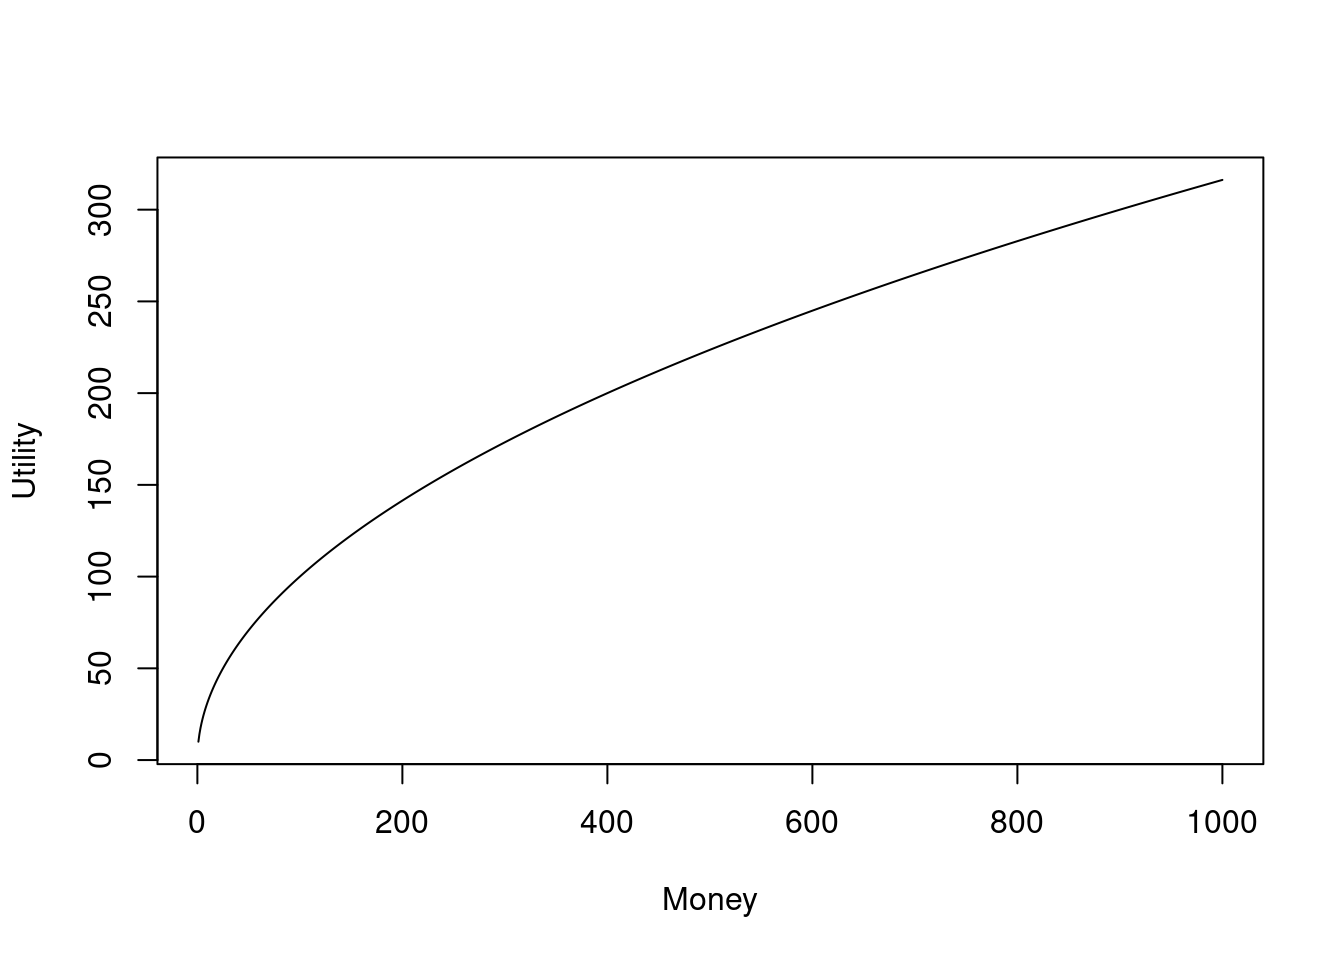
\includegraphics{decisiontheory_files/figure-latex/unnamed-chunk-4-1} \caption[Notice that the first 200 dollars get a rise in utilities that's about 140, but the next 200 dollars (from 200 to 400) only get a rise of about 60 utilities]{Notice that the first 200 dollars get a rise in utilities that's about 140, but the next 200 dollars (from 200 to 400) only get a rise of about 60 utilities.}\label{fig:unnamed-chunk-4}
\end{marginfigure}

\newthought{The fact that marginal utilities decline} means that money and utilities don't have a one-to-one relationship.\footnote{If it were a one-to-one relationship, we would have a straight diagonal line in our plot instead of a curved one.} And because money and utilities don't even have a one-to-one relationship, they can't be identified as the same thing, even if there seems to be some kind of indirect relationship between them.

\newthought{This indirect relationship between money and utilities} can be used to justify certain taxation policies.\footnote{The history of taxation is a complicated one and the point to be made here is meant to be only illustrative, so we'll ignore numerous complications.} Taxation is a way to help support society at large by funding projects that are beneficial to its members on aggregate (think roads, sewage, public spaces, etc). Except in very special circumstances, here's a bad way to fund projects: have a flat fee that each person pays each year, regardless of their income. Suppose the flat fee is \$1K per year. Superficially, it seems that this is fair, since both the person earning \$10,000 (call him Tim) and the person earning \$1,000,000 (call her Molly) are contributing the same dollar amounts through taxation. But a utility perspective shows that such taxation is not fair at all. The \$1K coming from Tim means he has \$9,000 left after taxes, while Molly has \$999,000. If we look at their respective \emph{loss} of utilities from the decreases in their spendable income, Tim is giving up more than Molly. To see this really clearly, imagine someone who only makes \$1,000 (or no money at all) - they would have nothing after the flat tax fee (or even be in debt because of it!). Given these kinds of considerations, we can see why there are plausible reasons for taxing the rich ``more'' than the poor.\footnote{We put `more' in scare quotes because, while it is more from a monetary perspective, that may not hold from a utility perspective.}

\newthought{The relationship between money and utilities} is actually far more curious than what declining marginal utilities suggest. We just saw how getting more money doesn't lead to an equivalent amount of utility. There are also examples where utility seems to be undermined by the mere introduction of the possibility of representing utilities with money.

For example, suppose a friend asks you for help to move apartments. You consider this to be a favour, one that you expect your friend to return when you move. We can see this as a kind of `tit-for-tat' exchange of utilities: the payoff you get for helping is the promise of getting help in the future (not to mention all the warm fuzzy feelings that come with helping another person generally, let alone just common decency).

But now suppose that your friend offers you one dollar for every hour that you help. From one perspective, that should sound like a great deal: you get all the benefits we just mentioned above, plus an extra two dollars for every hour of your time!

Most people, however, do not see it this way. Once your friend offers you the \$2/hr rate, you're likely to start thinking about what your time is worth in monetary terms, and your friend's offer is likely to be insulting to you. So, where from a naive perspective we might expect that the offer of money increases your preferences for the outcomes related to helping, it can actually have exactly the opposite effect. Somehow, for whatever reason, the introduction of money, even just the suggestion of it, can be parasitic on utilities related to social norms.

\newthought{Here's an interesting twist.} Imagine instead of money, your friend offered you beer instead (or whatever your beverage of choice may be). As long as your friend doesn't mention that the monetary value of the beer is equal to the \$2/hr rate, it's likely that you view the offer as more than fair. But if the beer is playing the role of monetary exchange, then you'd probably ask for more if you think your hourly rate is more than \$2.

If your intuitions about this example are in line with this narrative, then it's consistent with empirical findings concerning favours, gift giving and monetary exchange. (CITE ARIELY) As long as money is not mentioned, social norms dictate some roughly fair exchange of social utilities: I help you knowing that in the future there's a good chance I can count on you to reciprocate. But once money gets introduced, we tend to switch over to a very different way of thinking about the exchange.

These examples are not meant to suggest that there is no relationship between money and utilities. The point is that, at the very least, there is no straightforward way to substitute between money and utilities. So with that in mind, we turn now to consider what utilities might be.

\hypertarget{hedonism-and-experience-based-theories}{%
\subsection{Hedonism and Experience-based Theories}\label{hedonism-and-experience-based-theories}}

\newthought{What makes something good?} Or what makes it bad? Jeremy Bentham identified the good with pleasure and the bad with pain. On this view, we tend to avoid painful experiences because pain is identical to badness, and we tend towards good experiences because the good and pleasure are one in the same. This view gives us a neat little picture: someone's welfare is high if they have lots of good experiences and few bad ones, and welfare decreases as the number of good/pleasurable experiences go down while the number of bad/painful experiences go up.

It doesn't take long to realize that this picture gets complicated quite quickly. That is, we can find ways in which changes in pleasurable or painful experiences don't neatly track changes in welfare. For example, earning money can be a painful experience, quite literally if your job involves hard manual labour. And yet at the same time, that person might say that their welfare is going up. They may even say that their welfare is going up \emph{because} they have to endure some painful experiences.

We might say that's not quite right. After all, it's not difficult to imagine that someone might be able to increase their welfare even further if their job were less painful. Then again, if the job were less painful, the pay may go down accordingly. At the very least, what we can say thus far is that there is not some simple relationship between pleasurable/painful experiences and welfare - we can imagine welfare go up even with the introduction of some painful experiences.

There is an argument that, even if we introduce a host of complications, there simply is no account to be given that definitively connects welfare to the level of pain or pleasure of our experiences. The argument comes from a thought experiment from Robert Nozick called \emph{the experience machine}. Here's a version of this argument.\footnote{Nozick's thought experiment was written in 1974, before the movie \emph{The Matrix} came out in 1999. But if you've seen the movie you can easily imagine the sort of scenario that Cypher discusses.} We are asked to imagine a matrix-like situation in which a machine provides our brain with all the experiences of a good life - whatever that might mean to you. Like in the matrix, these experiences are not just sensations. The experiences are just like the ones we would have in real life, including the relationships we have with friends and family. The only difference is that the interactions weren't with real people. But we don't know that while in the experience machine. To the best of our knowledge, we can't tell the difference whether our friends and family actually died and they're just being simulated perfectly, or whether our interactions are with real individuals.

\newthought{Nozick argues} that a person that's lived a life in the experience machine has lead a bad life. Why? Because their entire world has been based on an illusion. While it is true that the person in the experience machine doesn't know the difference, if we were to take them out of it, it is likely that they would agree with us that the illusory nature of the experiences they had undermines the level of welfare they would assign to those experiences. If you think that welfare and good experiences track each other perfectly, then you would have to maintain the position that the person living in an experience machine lead a good life.

Notice that the argument isn't saying that experiences don't matter to welfare or the good life. Rather, the argument is saying that the character of our experiences is not all there is to a good life. That is, good experiences might be necessary to a good life, but they are not sufficient. What the experience machine argument is supposed to show is that one of the elements that's missing in an experience-based approach to welfare is the notion of experiences being \emph{real}.

Even if you don't find the experience machine argument compelling, there are other issues that remain. My experience of listening to heavy metal may produce pleasure, while it may produce pain in you. The fact that it feels good to me but bad to you suggests that we can't be having the same experience. If that's right, then we have to say that there are two different types of experiences being had while you and I listen to the same heavy metal track.

If that's not right, that is, if there is only one type of experience being had, is there anything that can be said to explain the difference in how you and I perceive the goodness and badness? One attempt might be to distinguish between lower and higher order experiences. That is, we might be having the same lower order experience of the music (this might be something like the `raw' perception of the music) but we could be having different higher order experiences. I might have a higher order experience of the lower order experience of violent drumming as an expression of existential angst, which feels good to release, while your higher order experience of the drumming might remind you of the frustrations of learning to ride a bike.

There are some good reasons for thinking that our experiences have these multiple levels happening in parallel. The smoker might know very well that they are engaging in risky behaviour, but at the same time that risky behaviour could be providing them with a higher order thrill. That might also be what's going on for some people when they watch horror movies.

\newthought{But not all experiences} seem to have such multiple levels. When I taste a scotch whisky from Islay (Scotland), I think the the salty, smoky, burnt rubber flavours are \emph{good}, while many people think those exact same flavours are \emph{bad}. And this difference doesn't seem to be one characterized by differences in higher order experiences. That is, our differences in tastes of scotch seem to be just at the lower order. If it's right, then the challenge for the experienced based view is to resolve the contradiction that the experience is good for one person but bad for another (given that the bad and the good are identified with experiences).

There are additional concerns with the experience-based view concerning the nature of time. A good experience today seems better than the same good experience 10 years in the future. This is not unlike the case of how money works, but it is more general and called \emph{discounting the future}.

Suffice it to say here that a purely experience-based view doesn't distinguish between the goodness or badness of an experience relative to your current point in time, and yet we do seem to behave in such a way that the present and near future are somehow different than the distant past or future.

\hypertarget{objective-list-theories}{%
\subsection{Objective List Theories}\label{objective-list-theories}}

Objective list theories start with the recognition that welfare may not be an aggregation of something simple, like a collection of pleasurable experiences. Rather, objective list theories recognize that welfare is a heterogeneous collection of things. We might have something like the following list:

\begin{itemize}
\tightlist
\item
  Good health
\item
  Shelter
\item
  Being in loving relationships with family and friends
\item
  Experiencing beauty
\item
  Engaging in virtuous behavior
\item
  Being rational
\item
  Acquiring knowledge
\item
  Doing things that make a life good, including things on this list
\end{itemize}

The approach to welfare as a multi-faceted concept is supposedly a strength of objective list theories, but it can also be seen as its primary weakness. There are a few ways to making the objection.

In order for any of the decision making rules to work, they need to assign a number to an outcome. So somehow, the information that's on a list has to be converted into a single unit of measurement - a utile. A list by itself doesn't tell us how to aggregate that information. So in order for an objective list theory to work for the decision making rules we've considered, it has to also provide such a procedure.

\newthought{There are reasons} for thinking that there is no plausible procedure for converting lists into utilities. For one, the very items on a list don't seem to be fixed. Different people might have different items on the list (perhaps we should then call it \emph{subjective} list theory). Or, even if the items on the list are the same, different people might weight the items differently. An academic and an athlete are likely to give different weights to acquiring knowledge and good health. So a procedure for converting lists has to deal with the fact that lists might differ in both the items that are on them and the weights to assign to items.

In order for any procedure to have the capacities just stated, there has to be a way for items on the list to be compared. The main thrust of the objection capitalizes on this requirement and it can be represented in the form of a dilemma.

\newthought{On the first horn}, there is no way of making comparisons between the items such that they can be aggregated into a single number. On this horn objective list theories concede that they can't provide an account of utilities for the purposes of decision making.

\newthought{On the second horn}, there is a way of making a comparison between the items. Comparisons are only possible if the items have something in common, some way of relating them to one another. But if they have something in common, then why not use whatever that is as a basis for utilities? For example, if the thing in common between experiencing beauty and being in a loving relationship is that they produce pleasurable experiences, then why not just use the experienced-based approach in the first place? On this horn of the dilemma, objective list theories give up the very idea that motivated them in the first place: that welfare is heterogeneous and multi-faceted.

\newthought{In brief:} if welfare is so heterogeneous that the items on the list cannot be compared, then the first horn is faced, but if items can be compared, then the second horn is faced. On either horn, objective list theories aren't the right account to provide a measure of utility.

\hypertarget{preference-based-theories}{%
\subsection{Preference-based Theories}\label{preference-based-theories}}

\newthought{One objection common} to both objective list theories and experience-based theories is that different people can have different views on what is good for them. That is, what counts as good for me can differ from what counts as good for you. One way to think of this is to say that welfare is something that is subjective, not objective.

Preference-based theories take this kind of objection seriously. On these accounts, what counts as good is that a preference is satisfied. \(A\) is better than \(B\) for an agent if and only if \(A\) is preferred to \(B\) by that agent. If we are talking about some other agent where \(B\) is preferred to \(A\), then for that agent \(B\) is better than \(A\).

Before we consider some complications of this approach, it's worth noting several advantages. As we already noted, a preference-based theory can handle the issues we raised earlier: that what increases welfare for one person (like our athlete) may not be what increases welfare for another (like our acaedmic).

But another substantial advantage is that preferences can be both nuanced on the one hand, and provide a unifying measure that we can use for utilities. For example, it has no problem handling differences in how people weight different items, or the times at which they would like for the items to be instantiated. For example, one person may prefer a steady stream of somewhat pleasurable experiences, while another enjoys a roller coaster of ups and downs in life. Preference-based theories are sufficiently general to account for such differences.

One serious complication of this view, however, comes from the idea that people could be wrong about what's good for them. On a purely subjectivist view, whatever a person desires is what's good for them, and vice versa. It seems perfectly reasonable, however, to say that sometimes people don't know what's good for them. Sometimes we think we know what's good for us, but we're actually wrong about that. Sometimes our preferences are challenged by other people. Anyone that has had the thoughts, ``I wish I didn't drink so much'' or ``I wish I didn't smoke'' are good examples of this.

So the trouble is, we want to be able to say both how welfare can be differential across individuals, but at the same time we want to be able to account for the fact that individuals could be wrong about what's good for them. Surely the right answer is somewhere in between. We don't expect utilities to be entirely subjective, nor entirely objective. Call this the subjective-objective \emph{tension} (as opposed to dilemma, which would suggest we have to pick one or the other).

\texttt{r\ newthought("One\ of\ the\ advantages")} of the preference-based approach is that it needn't be purely subjectivist. In fact, one of its chief advantages is that we needn't wait for a resolution in the debate about how to balance the two sides of the subjective-objective tension. All that a preference-based approach demands is that some \emph{minimal} criteria be met about what preferences are \emph{for an individual}. Decision theory, as we're considering it, is about how an individual should decide \emph{given their preferences} (recall our discussion of instrumental rationality). It thereby sidesteps some of the issues regarding interpersonal comparisons. In the next chapter we'll look at what the minimal criteria are and arguments for and against them.

\hypertarget{applications-and-challenges}{%
\section{Applications and Challenges}\label{applications-and-challenges}}

Whatever view you might be attracted to about cardinal utilities, let's have look at an application of them that is not available if we just used ordinal utilities. This is called the \emph{minimax regret rule}. After examining that rule, we consider some challenges of trying to distill down utilities into a single number.

\hypertarget{minimize-regret}{%
\subsection{Minimize Regret}\label{minimize-regret}}

A simple thing we can do with cardinal utilities is give a rough measure of regret. Let's consider an example. Suppose your options are to party, study, or call your family. Suppose further that tomorrow's exam will be either very difficult, medium difficult, or easy. Let's say that you assign the following utilities to the nine possible outcomes.

\begin{longtable}[]{@{}lccc@{}}
\toprule
& Very Difficult & Medium & Easy Exam\tabularnewline
\midrule
\endhead
\textbf{Party!} & 1 & 5 & 20\tabularnewline
\textbf{Study!} & 15 & 10 & 3\tabularnewline
\textbf{Call Family} & 7 & 8 & 9\tabularnewline
\bottomrule
\end{longtable}

There are different ways of thinking about regret. Here's one plausible way. Given a particular state, the amount of regret of an option is the difference between the highest outcome among all the options (under the given state) and the option under consideration. For example, under the state Easy Exam, the option to party has the highest outcome. So, the option to party has a regret of 0, the option to study has a regret of 17, and the option to call family has a regret of 11. Using the same strategy, we can calculate the amount of regret for the options under each of the other states. We then get the following \textbf{table of regrets}:

\begin{longtable}[]{@{}lccc@{}}
\toprule
& Very Difficult & Medium & Easy Exam\tabularnewline
\midrule
\endhead
\textbf{Party!} & 14 & 5 & 0\tabularnewline
\textbf{Study!} & 0 & 0 & 17\tabularnewline
\textbf{Call Family} & 8 & 2 & 11\tabularnewline
\bottomrule
\end{longtable}

Using this regret table, the \textbf{minimax regret} rule says to \emph{min}imize the \emph{max}imum possible regret. The strategy proceeds in two steps: first, find the maximum regret for each option (for Party! it's 14, for Study it's 17, and for Call Family it's 11), then second, pick the option with the lowest regret (in our example it's Call Family).

The minimax regret rule seems intuitive enough. Given the preference assignment, we really prefer to party if the exam is easy, and we really prefer to study if the exam turns out to be very difficult. The option to call family lies somewhere in the middle: no matter how hard the exam turns out, it feels pretty good to get encouragement from talking with family. But we are uncertain about how difficult the exam will be. Because we're uncertain, and under the assumption that we would rather not regret our choice, our best bet is to call family.

\textbf{Independence of Irrelevant Alternatives}

There is a principle called \emph{independence of irrelevant alternatives}, or IIA. The basic idea is that if you choose a specific option, like Call Family above, then removing one of the other options shouldn't change the recommendation. More formally, if option \(x\) is recommended among a set of options \(T\), then if \(S\) is a subset of options from \(T\) and \(x\) is a member of \(S\), then \(x\) should still be the recommended option.

It turns out that the minimax regret rule does not obey IIA. If it did, then that means the option to call family would still be recommended even if we ignored the option to go to the party (maybe it was canceled last minute). But we can show that minimax regret actually changes its recommendation.

To show this, we first take a subset of our previous options and make sure that Call Family is still a member of that subset. We can do this by deleting the option to party from the table above. That gets us this next table.

\begin{longtable}[]{@{}lccc@{}}
\toprule
& Very Difficult & Medium & Easy Exam\tabularnewline
\midrule
\endhead
\textbf{Study!} & 15 & 10 & 3\tabularnewline
\textbf{Call Family} & 7 & 8 & 9\tabularnewline
\bottomrule
\end{longtable}

Next we create our new regret table. Notice that this time we'll get different numbers under the Easy Exam column. This is because the highest outcome is no longer the one where we party and the exam is easy (20) - we've removed the party option altogether and thereby the corresponding outcomes. So now the highest outcome under Easy Exam is 9. In the other two columns, the highest outcomes are still the same (they are the study row). When we create the regret table, we then get the following.

\begin{longtable}[]{@{}lccc@{}}
\toprule
& Very Difficult & Medium & Easy Exam\tabularnewline
\midrule
\endhead
\textbf{Study!} & 0 & 0 & 6\tabularnewline
\textbf{Call Family} & 8 & 2 & 0\tabularnewline
\bottomrule
\end{longtable}

Following the minimax regret rule, we see that Study has a maximum regret of 6 while calling family has a maximum regret of 8. Picking the minimum of these leads to the recommendation of studying, the opposite of the recommendation it gave when we considered that the party was still on.

If we think that the Independence of Irrelevant Alternatives principle is correct, then that speaks unfavourably to the minimax regret rule. It is not obvious, however, that we should accept IIA. Here are two arguments why we might not accept IIA.

\texttt{r\ newthought("The\ first\ argument\ against\ IIA")} comes from empirical considerations. People seem to systematically behave at odds with IIA. A famous example is known as \emph{the decoy effect}.\footnote{CITE Kahnemann, CITE Ariely} Suppose you are deciding between two sandwiches, a small one (say a 6 inch loaf) vs a large (say 12 inch). The small is \$6 and the large is \$10. Between these two options, let's suppose that your preference is for the small sandwich - it's enough to fill you up and costs less than the large sandwich. Now imagine that the store announces a limited time medium sandwich, coming in at 9 inches and \$9. A lot of empirical work suggests that your disposition towards the large sandwich changes with the introduction of the medium sandwich, even if you don't actually have a preference for the medium sandwich. That is, in many cases people will opt for the large sandwich when the medium sandwich is present, but they prefer the small sandwich when it is not, even though the medium sandwich is not preferred. The medium sandwich is called the decoy.

Once you see it, you'll start noticing the decoy effect in a lot of places, especially in advertising. The effect is not restricted to marketing, however. Its applications are broad, even in dating. Suppose you see Jordan and Taylor at a party and you have a romantic interest in each of them. You find both equally attractive. You know Jordan is a great piano player while Taylor is a great guitar player. You have a bit of a soft spot for piano players, so you're inclined to strike up a conversation with Jordan (i.e., you have slight preference for Jordan over Taylor). But just as you head in Jordan's direction, you hear Taylor strumming along to a tune with one of their guitar playing friends, Kennedy. It's clear that Taylor is a more talented player than Kennedy. Research suggests that because you can compare Taylor to Kennedy - Kennedy is the decoy in this case - your preference can switch from your interest in Jordan to Taylor. Kennedy is irrelevant - you have no romantic interest in Kennedy - but their mere presence can affect your preferences. Of course, you hope that you're not the decoy for the friend who invited you to the party.\footnote{CITE Dan Ariely}

Just because the decoy effect is widespread, however, does not make it a definitive point against IIA. It is possible to say, in IIA's defense, that people are systematically failing to be rational. How much one takes seriously the empirical data in informing theoretical choices will depend in part on how descriptive and normative aspects of decision theory interact. As a descriptive theory, IIA fails to hold, but as a normative theory we may endorse IIA and point to the decoy effect as a systematic failure on our part to be ideal decision makers (just like some of us systematically fail at parallel parking).

\newthought{The second argument against IIA}, however, comes from theoretical considerations. The thought is that even as part of a normative theory, IIA is too strict of a requirement for rationality. One might think, for example, that when we are considering our options, we should do so holistically. That is, we should not just be comparing options pairwise or side by side until we have a winner. Rather, we should be comparing options as an entire collective. Put differently, when we are considering an option, we should be comparing it to the entire set of alternatives. If that's right, then even the ideal decision maker would violate IIA.

For example, suppose you collect vinyl records and you're on vacation somewhere to visit a vinyl shop. You see two records, both of which tend to be difficult to find. Let's say you prefer record A over record B. As you head to the counter with A in hand, you overhear some people talking about a stash of counterfeits that have been made of A. Such a copy, call it C, is widely available, is also at the store as a kind of gimmick, and it's noticeably ``cheaper looking'' than A. So let's say you prefer A over a copy C, and you also prefer record B to C. To many people it seems perfectly reasonable to think that the popularity of C makes A look less attractive, such that your preferences shift to prefer B over A. After all, B is more unique, seeing as it's not the sort of thing that there are as many copies of. (Similarly, we might run the story the other way so that instead of there being copies of A, there are lots of copies of B, but this time the fact that there are more copies makes B more special to you because you would have an original.)

We'll see other theoretical arguments against IIA in more detail when we look at the Allais paradox. To appreciate that argument, we first need to understand the rule for maximizing expected utility, which we'll cover in the next chapter. The key difference we'll see between maximizing expected utility and the rules we've looked at in this chapter has to do with how they incorporate uncertainty. But first, let's look at one more application of cardinal utilities.

\hypertarget{multiattribute-approach}{%
\subsection{Multiattribute Approach}\label{multiattribute-approach}}

In a single-attribute approach, we are forced to make direct comparisons when making decisions. This leads to us making comparisons between things like lives and money: at what point is the dollar cost of a search and rescue too high to save the lives of a few teenagers lost at sea? Here we are placing money and lives and a single utility scale.

In a multi-attribute approach, we allow for there to be multiple scales. Which scales are used depends on the attributes relevant to the decision. In the above example, we might use money to measure the financial costs of a search and rescue, and use number of lives saved as the scale for human welfare. The next step is then to determine how to aggregate the attributes into some overall ranking.

Here's an example. Suppose a politician is deciding on extending the search and rescue mission for the teenagers lost at sea. There are three attributes under consideration: the cost in dollars for each day of search, the number of lives saved, and the political implications (e.g., getting or losing votes). The politician is considering three options: end search, extend search one week, extend search indefinitely. For simplicity's sake, we're going to imagine that there's only one overarching world state (say, that the teenagers are still alive). For each outcome, the politician could use an ordinal ranking (i.e., a 1 means least preferred, not 1 life saved). Note that even though there is only one world state at the moment (Teens Alive), the outcome for End Search and Teens Alive has three compartments, one for each of the three attributes.

\begin{longtable}[]{@{}lccc@{}}
\toprule
& Money & Lives & Votes\tabularnewline
\midrule
\endhead
\textbf{End Search} & 3 & 1 & 1\tabularnewline
\textbf{Extend One Week} & 2 & 3 & 2\tabularnewline
\textbf{Extend Indefinitely} & 1 & 2 & 3\tabularnewline
\bottomrule
\end{longtable}

Unfortunately for the politician, there is no dominant option; dominance reasoning will not provide guidance for what to choose
The politician is not limited to the ordinal scale, however. We could instead use an interval (or quantitative) scale. By interpreting the numbers in the above table as cardinal numbers, we can then weight the values of the outcomes with how important each attribute is.

\textbf{Weighting by additivity}

In order to assign weights, we need to assume that they are additive and that the sum of the weights is equal to 1. Let's suppose that each attribute is equally important as any other. Then since we have three attributes, each one is assigned 1/3. The value of an option for the overarching outcome is then the weighted sum of its subdivided outcomes. For example, the option Extend One Week has a value of \(2\times 1/3 + 3 \times 1/3 + 2 \times 1/3 = 2.333\). Performing the analogous calculations for the other two options reveals that Extend One Week has the maximum value.

\begin{longtable}[]{@{}lcccc@{}}
\toprule
& Money (1/3) & Lives (1/3) & Votes (1/3) & Aggregate\tabularnewline
\midrule
\endhead
\textbf{End Search} & \(3\times \frac{1}{3}\) & 1\(\times \frac{1}{3}\) & 1\(\times \frac{1}{3}\) & =1.667\tabularnewline
\textbf{Extend One Week} & \(2\times \frac{1}{3}\) & 3\(\times \frac{1}{3}\) & 2\(\times \frac{1}{3}\) & =2.333\tabularnewline
\textbf{Extend Indefinitely} & \(1\times \frac{1}{3}\) & 2\(\times \frac{1}{3}\) & 3\(\times \frac{1}{3}\) & =2.000\tabularnewline
\bottomrule
\end{longtable}

Suppose instead that Votes is the most important thing for the politician. We might say, for example, that votes are twice as important as lives, and lives in turn are twice as important as money, i.e., Votes are weighted 4/7, Lives at 2/7, and Money at 1/7. Using these weights the Extend One Week option has a (rounded) value of 2.286, but the Extend Indefinitely option has a (rounded) value of 2.429. So different weightings of the attributes can lead to different recommendations.

\begin{longtable}[]{@{}lcccc@{}}
\toprule
& Money (1/7) & Lives (2/7) & Votes (4/7) & Aggregate\tabularnewline
\midrule
\endhead
\textbf{End Search} & \(3\times \frac{1}{7}\) & 1\(\times \frac{2}{7}\) & 1\(\times \frac{4}{7}\) & =1.286\tabularnewline
\textbf{Extend One Week} & \(2\times \frac{1}{7}\) & 3\(\times \frac{2}{7}\) & 2\(\times \frac{4}{7}\) & =2.286\tabularnewline
\textbf{Extend Indefinitely} & \(1\times \frac{1}{7}\) & 2\(\times \frac{2}{7}\) & 3\(\times \frac{4}{7}\) & =2.429\tabularnewline
\bottomrule
\end{longtable}

Don't forget that the columns in this table are all under the state assumption of Teens Alive. You'll have something similar for the state Not Alive. Later we'll see how we can combine states and utilities by using probabilities, but that's in the next chapter.

\textbf{Non-additive strategy and general challenges}

This weighting strategy of the multi-attribute approach assumes that the attributes are additive, i.e., that their relative importance can be summed. Consider again a criticism of the completeness axiom, which can be launched similarly here. The aggregation of attributes on a scale from 0 to 1 that sum in total to 1 is no different than comparing objects on a single scale. It's the same problem, we've just moved from comparison of objects to comparisons of attributes.

Using non-additive criteria is one strategy for sidestepping the above objection while still handling incomplete preference orderings. Suppose each attribute has an \emph{aspirational level} such that if that minimum level is not achieved, then the corresponding option or alternative is disregarded, even if that option ranks highly in other attributes. For example, suppose that we set the aspirational level for each of the attributes above at 2. Then End Search and Extend Indefinitely will be disregarded because each of them has at least one outcome below 2. Notice that on this strategy the attributes aren't being compared on some single scale. Each attribute gets to set its own level and then we check to make sure that the options meet that minimum level.

A severe complication of this non-additive strategy is specifying aspirational levels for each attribute: there seems to be both arbitrariness and vagueness to the levels.

There are concerns related to multi-attribute approaches generally. Without some theory for individuating attributes, it is possible that the strategy leads to conflicting recommendations (whether or not they are additive). For example, suppose that a medical products agency is deciding whether to approve a new hand cream. It is unknown whether the long term effects of the hand cream leads to increased toxicity. Toxicity may then be taken as a relevant attribute. Let us suppose that while for half the population the hand cream increases toxicity, for the other half of the population the cream actually leads to a decrease in toxicity. We can suppose that whether it does or doesn't depends on something genetic. If we conceive of toxicity as a single attribute, then the average increase in toxicity is zero because one half of the population cancels out the other. By these lights, the hand cream might get approved. It seems reasonable, however, to characterize toxicity in terms of two attributes: ``toxicity for people with gene A'' and ``toxicity for people with gene B''. If we individuate attributes in this way, the recommendation may be to not approve the hand cream if the risk for people with one of the genes is sufficiently large. So here is an example where there are two different ways of aggregating risks that lead to conflicting recommendations, and since we have no way of determining which is the correct way of individuating attributes, a multi-attribute approach does not solve the problem of dealing with incomplete preference orderings.

\hypertarget{more-challenges-and-final-remarks}{%
\section{More Challenges and Final Remarks}\label{more-challenges-and-final-remarks}}

There is much more to be said about the notion of utilities. Even in the more minimal case of preference-based theories, we assume that they are transitive and complete. Moreover, we have implicitly assumed that a person knows what their own preferences are, at least in the moment. But there are good reasons for thinking that in many scenarios we \emph{don't} know our own preferences and look towards others to either discover or create our own. We also have reasons for thinking that preferences can change over time, and in some cases it seems that the way our preferences change is not predictable beforehand.

Even if individuals had unchanging preferences that they knew perfectly, there are good reasons for treating utilities across time differently. It seems plausible to think that a unit of utility is more valuable today (from your perspective on the present day) than it is ten years from now. After all, there's no guarantee that you'll live another ten years to obtain that unit of utility, and it's far more likely that you'll live through today. Investing money illustrates a similar idea quite nicely. \$1,000 dollars today is worth more than \$1,000 next year (even if we increase this amount to account for inflation) because you can invest it today and turn it into more than \$1,000 by next year (market crashes notwithstanding). For these sorts of considerations, we often \emph{discount} our future selves in the decisions we are making in the present. That is, while it is important to think about yourself in the future, the preferences of your future self should not be given the same weight as you in the present. Again, who knows if your future self even comes to be: as the famous economist Maynard Keynes said, ``In the end we are all dead.''

Interesting, it's not clear whether we should apply the same sort of thinking when we are considering decisions at the aggregate or group level. Unlike the guarantee that your life will come to an end and we have a decent sense of how long you will \emph{not} live, the life of communities is far more open-ended. In fact, society is likely to go on far longer than individuals that it makes sense to model society as if it were to go on forever - this is sometimes referred to as the `infinite life' assumption in economics. Without an endpoint in sight, it's not clear how much we should be discounting future generations. In fact, some philosophers and economists suggest that, given that we have some moral obligations to future society, we shouldn't discount future generations at all. Frank Ramsey said, ``In time the world will cool and everything will die, but that is a long time off still, and its present value at compound discount is almost nothing.'' So while the death of individuals warrants the application of a discount function, the death of society is so far off that the "same'' reason does not apply here. Once again we see there is a kind of discontinuity between decision making at the level of individuals and the level of groups.

All of these considerations raise interesting questions about how preferences affect decision making. But we need to return to the idea of an \emph{expectation} in the first place. To do that, it is not enough to just think in terms of utilities. We have to be more explicit about the notion of a probability, like we used in lottery option procedure, and how they are used in models of decision making. We turn to that next.

\hypertarget{exercises-3}{%
\section*{Exercises}\label{exercises-3}}
\addcontentsline{toc}{section}{Exercises}

\begin{enumerate}
\def\labelenumi{\arabic{enumi}.}
\item
  Suppose we have a utility scale that goes from 0 to 5 and we're trying to determine what utility Alice assigns to an option called \(D\). We know that Alice has the preference ordering of \(A\succ D \succ C\). Suppose we present Alice with a lottery option \(L\) and we determine that Alice said \(D \sim L\) when \(L\) consists of 60 tickets of \(A\) and 40 tickets of \(C\).

  \begin{itemize}
  \tightlist
  \item
    What utility does \(D\) have for Alice assuming that \(A\) is 5 and \(C\) is 0?
  \item
    What if instead \(A\) is 4 and \(C\) is 3?
  \end{itemize}
\item
  Which interpretation of cardinal utilities (hedonism, objective list theory, or preference-based) do you find most compelling? Why?
\item
  Provide an application of the minimax regret rule to one of your own decisions. Remember you will need two tables, one is the standard utility table, the second is the table of regrets (which you calculate from the utility table).

  \begin{itemize}
  \tightlist
  \item
    Does the recommendation of the minimax regret rule correspond with your intuition about what to do?
  \item
    Does your example obey the principle of independence of irrelevant alternatives?
  \end{itemize}
\item
  Provide an application of the multiattribute approach to one of your own decisions, using weighting by additivity.

  \begin{itemize}
  \tightlist
  \item
    Does the recommendation of the multiattribute approach correspond with your intuition about what to do?
  \item
    If not, is there any way to update the weights so that it would?
  \item
    If so, how much could you change the weights so that the approach would make a different recommendation?
  \end{itemize}
\end{enumerate}

\hypertarget{expected-utilities}{%
\chapter{Expected Utilities}\label{expected-utilities}}

We developed the lottery option procedure to help us build interval scales for people's preferences, which lets us both order preferences and say how much more one thing is preferred to another.\footnote{Recall how the lottery option procedure worked: given options A\(\succ\)B\(\succ\)C, where A and C make up a lottery L, what percent of L's tickets need to be A in order for the person to be indifferent between A and B? The percent of A tickets is the percent of B's desirability of A.} But we noted a curiousity about this procedure. Saying that you prefer a lottery is quite a different thing than saying you prefer a particular outcome, like a book. It seems intuitive enough to think about selecting book B rather than another: we purchase it, put it beside our bed, read it, etc. But what does it mean to act on or choose a lottery? Yes, you can purchase a ticket. But you can't \emph{choose} the \emph{winning} ticket in the sense that your choice guarantees the ticket is a winning one. Whether your ticket wins or loses is the outcome of some chancy process. How can we make better sense of this?

The central concept that will help us here is \emph{expectation}. Informally, we think of expectations as strong beliefs that something will occur. When walking I almost always expect that the ground will support my weight. When I set my alarm I expect it to wake me up. When I work at my job I expect to get paid. These examples are in contrast to things we might \emph{merely} hope or desire to be true.

There is also a more technical meaning of what it is to have an expectation. Here we make use of the concept of probabilities in making a kind of measured prediction. We move away from a strong belief that something \emph{will} occur, and more towards what could occur to some degree of chance.

\hypertarget{expected-utility-by-example}{%
\section{Expected Utility by Example}\label{expected-utility-by-example}}

Here is an example. Suppose you have a rash on your hand. In half of all cases the rash goes away by itself, for the other half it doesn't. So, if you do nothing, there's a 50/50 chance the rash gets better. There's an over the counter cream you can use that helps the rash get better, but it's not perfect: 85\% of the time the rash goes away, but there's a 15\% chance that it continues even when using the cream.\footnote{We have to be careful that we're conceiving of the ``rash gets better'' state as those aspects of the cream that are outside of our control. The state can't be those aspects of the action that correspond to the use of the cream, otherwise we violate the constraint that states and options have to be independent. We have to think of the ``rash gets better'' state as those properties related to the efficacy of the cream that are outside our control - like the sensitivity of your skin.}

\begin{longtable}[]{@{}lcc@{}}
\toprule
& Rash gets better & Rash continues\tabularnewline
\midrule
\endhead
Use Cream & 85\% & 15\%\tabularnewline
Do Nothing & 50\% & 50\%\tabularnewline
\bottomrule
\end{longtable}

The notion of expectation that we are going to use combines this kind of information about probabilities with cardinal utilities. In fact, we'll have a new strategy called \textbf{maximize expected utility}, which will use information about how probable outcomes are, like in the table above, in combination with our utilities of those outcomes. That is, we use the probabilities \emph{to weight} a preference assignment.

To make the example easier, let's think of utilities in terms of money.\footnote{Some authors will distinguish between \emph{expected monetary value} and \emph{expected utility} in order to acknowledge the concerns we raised in the previous chapter. Here we're just trying to highlight how to think about \emph{expectation}, and so for most of this chapter we'll treat utilities and monetary value the same.} There are two costs we need to think about: the cost of the over the counter hand cream and the cost of seeing the doctor if the rash continues. (Strictly speaking, there is also a third ``cost'' if we assume that the price of doing neither is \$0.) Let's say that the cost of the hand cream is \$20 and the cost of going to the doctor is \$100. In the event that you tried the hand cream and it didn't work, you still have to go to the doctor (who may prescribe a stronger cream), so you're paying both costs. In terms of a preference assignment, we then get the following table.

\begin{longtable}[]{@{}lcc@{}}
\toprule
& Rash gets better & Rash continues\tabularnewline
\midrule
\endhead
Use Cream & -\$20 & -\$20+(-\$100) = -\$120\tabularnewline
Do Nothing & -\$0 & -\$100\tabularnewline
\bottomrule
\end{longtable}

If all that matters are these utilities, then we can apply the rules we used in the previous chapters. For example, dominance reasoning would tell us not to use hand cream because for each state, the option not to use cream is better (i.e.~less expensive) than the option to use cream.

But utilities are not all that matter. We also have other information: the probabilities of each of these outcomes.

The rule for maximizing expected utility proceeds in two steps:

\begin{verbatim}
-Step One: combine the utility and probability tables to calculate the expected utility of each option. 
-Step Two: select the option with the maximum expected utility. 
\end{verbatim}

Let's go through these separately.

\hypertarget{step-one-compute-eu-of-each-option}{%
\subsection{Step One: Compute EU of each option}\label{step-one-compute-eu-of-each-option}}

Here's how we calculate the expected utility of an option. First, for each outcome, multiple the utility of that outcome (using the utilities table) by the probability of that outcome (using the probability table). Second, take the sum of these products.

For example, to calculate the expected utility of using cream, I would first do this:

\begin{longtable}[]{@{}lcc@{}}
\toprule
& Rash gets better & Rash continues\tabularnewline
\midrule
\endhead
Use Cream & -\$20 x 0.85 & -\$120 x0.15\tabularnewline
\bottomrule
\end{longtable}

Which gives me this:

\begin{longtable}[]{@{}lcc@{}}
\toprule
& Rash gets better & Rash continues\tabularnewline
\midrule
\endhead
Use Cream & -\$20 x 0.85 = -\$17 & -\$120 x0.15 = -\$18\tabularnewline
\bottomrule
\end{longtable}

I then take the sum of these outcomes, which is -\$35. We say that the expected utility of using the hand cream is a \emph{loss} of 35 dollars (recall we're ignoring a bunch of complications for now, like whether the hand cream makes my hands feel greasy, how my hands smell, etc.). We'll represent this expected utility as \textbf{EU} and put it in as column to the very right, being careful not to interpret that column as another state.

\begin{longtable}[]{@{}lccr@{}}
\toprule
& Rash gets better & Rash continues & EU\tabularnewline
\midrule
\endhead
Use Cream & -\$17 & -\$18 & (-\$17) + (-\$18) = \textbf{-\$35}\tabularnewline
\bottomrule
\end{longtable}

We then do the same computation to calculate the expected utility of Do Nothing. So our complete table would look like this (showing the work for Do Nothing):

\begin{longtable}[]{@{}lccr@{}}
\toprule
& Rash gets better & Rash continues & EU\tabularnewline
\midrule
\endhead
Use Cream & -\$17 & -\$18 & \textbf{-\$35}\tabularnewline
Do Nothing & -\$0 x 0.5 = \$0 & -\$100 x 0.5 = -\$50 & (-\$0)+(-\$50) = \textbf{-\$50}\tabularnewline
\bottomrule
\end{longtable}

This makes up our first step.

\hypertarget{step-two-find-maximum-eu}{%
\subsection{Step Two: Find maximum EU}\label{step-two-find-maximum-eu}}

Once we have our table where we have calculated the expected utility for each option, we then look for which one is the maximum. We have to be a bit careful here, because the signs of the numbers matter, not just the magnitude. So while \$50 is more than \$35, what we are concerned with is avoiding the loss of money. In other words, when utilities are positive we want to take the largest one, but when utilities are negative we want to take the smallest one. In the current context the utilities are negative, so we are trying to maximize the least amount of loss. Hence the option with the maximum expected utility is Use Cream. We'll sometimes put an explanation point beside the maximum expected utility number.

\begin{longtable}[]{@{}lccr@{}}
\toprule
& Rash gets better & Rash continues & EU\tabularnewline
\midrule
\endhead
Use Cream & -\$17 & -\$18 & \textbf{-\$35!}\tabularnewline
Do Nothing & \$0 & -\$50 & \textbf{-\$50}\tabularnewline
\bottomrule
\end{longtable}

If two options have the same expected utility, and all other expected utilities are smaller than those options, then there is a tie. A common suggestion is that such ties mean that either option is equally as good (or least bad) as the other. We will see, however, that we might want to be more nuanced than merely maximizing expected utilities. For example, it's possible that two options have the same expected utilities, but one of them has a higher ``risk'' in that one of the outcomes has a very low utility, but also a very low probability. We will consider such possibilities shortly when we examine criticisms of the strategy of maximizing expected utilities.

\hypertarget{meu-maximize-expected-utility-strategy}{%
\section{(MEU) Maximize Expected Utility Strategy}\label{meu-maximize-expected-utility-strategy}}

It will be helpful to have some notation. Let's say that \(U(A|S_1)\) means "the utility of option A given state 1''. So we could write \(U\text{(Use cream}|\text{rash gets better})\) to refer to the \$20 cost. Or we could write it like an equation. Here's how we might refer to the case where we use cream and the rash continues:
\[
U(\text{Use cream} | \text{rash continues}) = -\$120
\]

In addition to using \(U\) to refer to utilities, we also need a handy way to refer to the probabilities of outcomes in a probability table.
Let's use \(P(A|S_1)\) to mean the probability of the outcome when option A is selected and state 1 occurs. So in order to refer to the chance that the rash gets better given that you use hand cream, which is 85\%, we would write

\[
P(\text{Use cream} | \text{rash gets better}) = 0.85
\]

Now that we have a way to refer to utilities and a way to refer to probabilities, we can write down a general way of how expected utilities are calculation. The expected utility of an option (say A) where there are two states can be written like this:\footnote{Don't forget your order of operations!}

\[
EU(A) = P(A|S_1)\times U(A|S_1) +  P(A|S_2)\times U(A|S_2)
\]

Plugging in the numbers from the table above for the hand cream option, we would get this:
\[
  \begin{aligned}
  EU(\text{Use Cream}) &= (0.85\times -\$20) + (0.15\times -\$120)\\
      &= -\$35
  \end{aligned}
\]

Similarly, the expected utility for not using the hand cream would be:
\[
  \begin{aligned}
  EU(\text{Do Nothing}) &= 0.5\times -\$0 + 0.5\times -\$100 \\
  &= -\$50
  \end{aligned}
\]

As illustrated in the above example, once we have calculated the expected utility for each option (i.e.~each row in our tables), then we pick the maximum of all the utilities. Note that this strategy works whether there are just two options, or if there are three, four, etc. The first step is a calculation of the expected utility for each option, which is done independently for each row. So the addition of another row doesn't make a difference to how the other options were calculated (well almost - we'll see later that we're making an important assumption here!). It's only in the second step that might be affected, but here we need to have calculated the expected utility for each option before we can go about selecting the maximum one.

\newthought{Note that we have a difference in recommendations} from some other rules. Dominance reasoning would tell us not to use the hand cream. But dominance reasoning ignores some important information about the chances of the different outcomes happening. One way to incorporate that information, in fact the most common way to do so, is to weight the utility of the outcome with the probability of that outcome.\footnote{The idea of ``weighting'' is what the operation of multiplication is doing here.} When we do that for each outcome for a given option and then add them up, we get the expected utility for that option. If we then compare the expected utilities of each option, at least for the example we've considered above, we get a different recommendation: don't use the hand cream.

The \emph{maximize expected utility} rule is the predominant strategy in the field of decision theory.\footnote{That's not to suggest it's always as simple as we've been illustrating, but it is at the heart of many decision analyses.} It is a very rich strategy. For example, we can actually recover the recommendation that dominance reasoning gave us. In order to do that, we ignore the information that using hand cream improves the chances of the rash getting better. We can represent this ignorance by giving each outcome for a given option the same probability. That is, we use the following table of probabilities:

\begin{longtable}[]{@{}lcc@{}}
\toprule
& Rash gets better & Rash continues\tabularnewline
\midrule
\endhead
Use Cream & 0.5 & 0.5\tabularnewline
Do Nothing & 0.5 & 0.5\tabularnewline
\bottomrule
\end{longtable}

Notice that the probability in a given row add up to 1. That's because the states are \emph{exhaustive} in each given option. That is, if I use the hand cream, my rash will either get better or it won't - there are no additional things that can happen. The same is true if I don't use it: either the rash goes away or it doesn't.

Now if we plug these numbers into our expected utilities, we get
\[
  \begin{aligned}
  EU(\text{use cream}) &= 0.5\times -\$20 + 0.5\times -\$120\\
  &= -\$70
  \end{aligned}
\]

and

\[
  \begin{aligned}
EU(\text{don't use cream}) &= 0.5\times -\$0 + 0.5\times -\$100 \\ 
  &= -\$50
  \end{aligned}
\]

Notice that when we take the maximum of these\footnote{Remember again these are representing \emph{costs}.} then the \emph{maximize expected utility} rule says not to use the hand cream. That's precisely the recommendation that dominance reasoning originally gave us!

The main takeaway is this. When we are in the context of making a decision under ignorance where we don't know what the probabilities of outcomes are, the dominance principle is usually the ``go to'' rule that is first tried (and sometimes it doesn't give us a recommendation). In the context of making a decision under known risk, we have information about the probabilities of outcomes and we use that information to calculate expected utilities, which in turn are maximized. Interestingly, we can use the decision rule of maximize expected utility to also represent the dominance strategy. We do this by "ignoring'' the probabilities of outcomes by making them all equally likely. In a rough way, then, maximize expected utility (MEU) is a generalization of the dominance principle, at least in terms of the recommendations MEU makes.

We say ``in a rough way'' because the recommendations that the dominance strategy and MEU make can come apart. In fact we have already seen this in the introduction. Recall \emph{Newcomb's Problem} where you can either pick the contents of just box A or the contents of both box A and box B. The utility table looked like this:

\begin{longtable}[]{@{}lcc@{}}
\toprule
& AI predicts two box & AI predicts one box\tabularnewline
\midrule
\endhead
\textbf{One box (just A)} & \$0 & \$1,000,000\tabularnewline
\textbf{Two box (A and B)} & \$1,000 & \$1,001,000\tabularnewline
\bottomrule
\end{longtable}

Dominance reasoning makes the recommendation to select the Two Box option, because whatever the AI predicted, you get an extra \$1,000. But dominance reasoning ignores the probabilities of each of the outcomes. In the description of the setup we said that there is a very strong correlation between what options people pick and what the AI predicts. So if you pick the One Box option, then the probability that the AI predicted that you would pick that option should be high, very high. It might not be perfect, but we can suppose that the AI is right 99\% of the time. So, the probability table might look like this:

\begin{longtable}[]{@{}lcc@{}}
\toprule
& AI predicts two box & AI predicts one box\tabularnewline
\midrule
\endhead
\textbf{One box (just A)} & 0.01 & 0.99\tabularnewline
\textbf{Two box (A and B)} & 0.99 & 0.01\tabularnewline
\bottomrule
\end{longtable}

Following the steps we outlined above for the MEU stragey, we get the following expected utilities for each option:

\[
\begin{aligned}
EU(\text{OneBox}) &=(0.01\times \$0) + (0.99\times \$1,000,000)\\
&= \$990,000
\end{aligned}
\]

\[
\begin{aligned}
EU(\text{TwoBox}) &=(0.99\times \$1,000) + (0.01\times \$1,001,000)\\
&= \$990 + \$10,010 \\
&= \$11,000  
\end{aligned}
\]

Let's add these to our utility table.

\begin{longtable}[]{@{}lccr@{}}
\toprule
& AI predicts two box & AI predicts one box & EU\tabularnewline
\midrule
\endhead
\textbf{One box (just A)} & \$0 & \$1,000,000 & \textbf{\$990,000!}\tabularnewline
\textbf{Two box (A and B)} & \$1,000 & \$1,001,000 & \textbf{\$11,000}\tabularnewline
\bottomrule
\end{longtable}

Clearly the One Box option has a much higher expected utility than the Two Box option! So, in contrast to the dominance strategy recommendation, the MEU strategy recommends that you should select just box A.

We have in a sense made interesting progress, and in another sense we have not. We have made progress in the sense that we can be more precise in how we describe the two different ways of reasoning about what do to in the Newcomb Problem. We have not yet made progress in providing an argument for whether we should use dominance reasoning or MEU. But the fact that we can be more precise about the two reasoning processes means we have a better understanding of what background assumptions each one is making. In turn, by analyzing those assumptions we can consider arguments for and against each of the two strategies. Much of the progress that has been made in decision theory has come from these kinds of analyses, which we'll cover in due time.

Next, we're going to look at an application of MEU that builds from a previous example.

\hypertarget{application-combining-meu-and-the-multi-attribute-approach}{%
\section{Application: Combining MEU and the Multi-Attribute Approach}\label{application-combining-meu-and-the-multi-attribute-approach}}

In the multi-attribute approach we covered, we showed how utilities might come from multiple scales. We used an example of a politician combining three scales (money, lives, and votes) to make a decision about a search and rescue mission for some teenagers lost at sea. The politician is considering three options: end search, extend search one week, extend search indefinitely, and we supposed that there were two possible states: Teens Alive and Teens Not Alive.

It was crucial in that example that we were focusing on just the state Teens Alive. As a reminder, the final utility table for the Teens Alive state was this:

\begin{longtable}[]{@{}lclclcl@{}}
\toprule
& Money (1/7) & & Lives (2/7) & & Votes (4/7) & Aggregate\tabularnewline
\midrule
\endhead
\textbf{End Search} & \(3\times \frac{1}{7}\) & + & 1\(\times \frac{2}{7}\) & + & 1\(\times \frac{4}{7}\) & =1.286\tabularnewline
\textbf{Extend One Week} & \(2\times \frac{1}{7}\) & + & 3\(\times \frac{2}{7}\) & + & 2\(\times \frac{4}{7}\) & =2.286\tabularnewline
\textbf{Extend Indefinitely} & \(1\times \frac{1}{7}\) & + & 2\(\times \frac{2}{7}\) & + & 3\(\times \frac{4}{7}\) & =2.429\tabularnewline
\bottomrule
\end{longtable}

What the aggregate utility in the very right column represents is the ``fusion'' of all the different scales (money, lives, votes) into a single utility value. To do that we weighted the utility of an outcome by how important the relevant scale (the column) was to the politician. Notice that the weights assigned to the columns here are \emph{not} the same as the probabilities that we use to weight utilities when calculating expected utilities of outcomes. To see this, notice that the decision problem for the politician needs to include both the Teens Alive state as well as the Teens Not Alive state. In other words, the full decision problem is given by the table below, which is only partially filled in using the aggregate values from the table above.

\begin{longtable}[]{@{}lccc@{}}
\toprule
& Teens Alive & Teens Not Alive & EU\tabularnewline
\midrule
\endhead
\textbf{End Search} & 1.286 & ? & ?\tabularnewline
\textbf{Extend One Week} & 2.286 & ? & ?\tabularnewline
\textbf{Extend Indefinitely} & 2.429 & ? & ?\tabularnewline
\bottomrule
\end{longtable}

In order to fill in the missing utilities under the Teens Not Alive column, we have to first use the multi-attribute approach to find the aggregate utility for each outcome under that state, using the same weighting as we did before. Recall that we supposed the politician thought lives are weighted twice as much as money, and that votes are weighted twice as much as lives. So we know what the weights are. What we need to do is figure out what the utilities are for the three options now that we're considering the state Teens Not Alive. This can be and probably would be different than the utility table we had from before. If the teens are not alive, then it seems that ending the search sooner would be better than later for all three scales: doing a search and rescue costs money, puts additional lives at risk, and voters aren't typically fond of wasting money. With that reasoning, the politician might use the following multi-attribute table for the Teens Not Alive state.

\begin{longtable}[]{@{}lccc@{}}
\toprule
& Money & Lives & Votes\tabularnewline
\midrule
\endhead
\textbf{End Search} & 3 & 3 & 3\tabularnewline
\textbf{Extend One Week} & 2 & 2 & 2\tabularnewline
\textbf{Extend Indefinitely} & 1 & 1 & 1\tabularnewline
\bottomrule
\end{longtable}

As before, the politician would then weight these to calculate an aggregate:

\begin{longtable}[]{@{}lclclcl@{}}
\toprule
& Money (1/7) & & Lives (2/7) & & Votes (4/7) & Aggregate\tabularnewline
\midrule
\endhead
\textbf{End Search} & \(3\times \frac{1}{7}\) & + & 3\(\times \frac{2}{7}\) & + & 3\(\times \frac{4}{7}\) & =3.000\tabularnewline
\textbf{Extend One Week} & \(2\times \frac{1}{7}\) & + & 2\(\times \frac{2}{7}\) & + & 2\(\times \frac{4}{7}\) & =2.000\tabularnewline
\textbf{Extend Indefinitely} & \(1\times \frac{1}{7}\) & + & 1\(\times \frac{2}{7}\) & + & 1\(\times \frac{4}{7}\) & =1.000\tabularnewline
\bottomrule
\end{longtable}

Now we can use those aggregate utility numbers to fill in the utilities under the Teens Not Alive state in our decision matrix:

\begin{longtable}[]{@{}lcrc@{}}
\toprule
& Teens Alive & Teens Not Alive & EU\tabularnewline
\midrule
\endhead
\textbf{End Search} & 1.286 & 3 & ?\tabularnewline
\textbf{Extend One Week} & 2.286 & 2 & ?\tabularnewline
\textbf{Extend Indefinitely} & 2.429 & 1 & ?\tabularnewline
\bottomrule
\end{longtable}

The maximize expected utility rule will now weight these utilities with the \emph{probabilities} of the states. Here is the place where the politician will need to collect some information about the world. They might consider success rates of past rescue efforts that are similar to this situation. They might consult some survival experts, locals who travel on the water in that area, weather reports, etc. Suppose at the end of all these considerations, the politician's assessment is that Teens Alive is three times more likely than Teens Not Alive, i.e.~that the Teens Alive state has a 75\% chance while Teens Not Alive has a 25\% chance. Now the politician can calculate the expected utilities for each option (rounding to four decimal places):

\begin{longtable}[]{@{}lclcc@{}}
\toprule
& Teens Alive & & Teens Not Alive & EU\tabularnewline
\midrule
\endhead
\textbf{End Search} & 1.286 x 0.75 & + & 3 x 0.25 & =1.7145\tabularnewline
\textbf{Extend One Week} & 2.286 x 0.75 & + & 2 x 0.25 & =2.2145\tabularnewline
\textbf{Extend Indefinitely} & 2.429 x 0.75 & + & 1 x 0.25 & =2.0718\tabularnewline
\bottomrule
\end{longtable}

The maximize EU rule then recommends that the politician extend the search for one week.

This example illustrates the richness of the maximize expected utility rule. It helps us organize a variety of considerations about a decision and tells us how to combine these into a recommendation. We first need to determine the utilities of each outcome, which we did using the multi-attribute approach. We then need to assess the probabilities of the states, which we gestured at here and we will return to in more detail shortly. MEU then tells us to weight the utilities by the probabilities of the states to arrive at a final expected utility for each option. There are many ways that real decisions introduce further complications, particularly in how to estimate the probabilities of states. But such complications don't change the underlying principle of MEU. It is no wonder that MEU is one of the most common ways of representing decision problems to make recommendations.

That said, we do have to take some care in the kinds of inputs we give to MEU. In the next section we'll illustrate this using a historical example.

\hypertarget{pascals-wager}{%
\section{Pascal's Wager}\label{pascals-wager}}

Let's see what happens if we assume that states can have probabilities of one or zero, or what happens if utilities can be infinite. We're going to use Pascal's Wager as an illustration of some concepts, not as an analysis of Pascal's actual argument, which is concerned about the relationship between faith and reason.\footnote{The Stanford Encyclopedia of Philosophy has a great entry on \href{https://plato.stanford.edu/entries/pascal-wager/}{Pascal's Wager.}}

In this wager, the states are either that God exists or God does not exist. The options are that we believe in God or we disbelieve. Let's set up the framework for our decision table:

\begin{longtable}[]{@{}lcc@{}}
\toprule
& God exists (G) & God does not exist (\(\neg\)G)\tabularnewline
\midrule
\endhead
\textbf{Believe (B)} & &\tabularnewline
\textbf{Don't Believe (\(\neg\)B)} & &\tabularnewline
\bottomrule
\end{longtable}

So far we haven't said anything about the probabilities of the outcomes nor the utilities. Let's think first about the utilities. Again, we're going to oversimplify for illustrative purposes. If God exists and I am a believer, then I go to heaven and have eternal life. Presumably heaven is a pretty good place where the ``party'' literally never ends - it goes on for eternity. So that means that the amount of utility I would get is infinite. Even if there are some bad days in heaven (but that's probably not true) the number of good days will be larger, and so the net amount is an infinite number of positive utilities, i.e., +\(\infty\). If, on the other hand, I don't believe in God and God does exist, then I will experience eternal hell, i.e., -\(\infty\).

What about the outcomes under the state where God does not exist? In that case my life is finite and the cumulative number of utilities I will experience, positive or negative, will also be finite. Now let's assume that being a believer comes with some costs: a believer volunteers their time when they'd rather be watching sports, or they give away a larger amount of their income to charity than a disbeliever, or they choose not to imbibe when they really would prefer to drink, etc. Let's say for a believer there is a finite net cost (-c) and for the disbeliever there is a finite net gain (+c).

From these assumptions, we have the following utility table:

\begin{longtable}[]{@{}lcc@{}}
\toprule
& God exists (G) & God does not exist (\(\neg\)G)\tabularnewline
\midrule
\endhead
\textbf{Believe (B)} & +\(\infty\) & -c\tabularnewline
\textbf{Don't Believe (\(\neg\)B)} & -\(\infty\) & +c\tabularnewline
\bottomrule
\end{longtable}

Before we try to add any information about the probabilities of outcomes, notice that the dominance principle does not make a unique recommendation. If God exists, it is better to believe than not to, and if God does not exist it is better not to believe than to believe.

In order to see what maximize expected utility (MEU) recommends, we have to include probabilities for the outcomes so that we calculate expected utilities. As a first approach, let's use the idea above to make each state equally probable. In that case we would have the following probability table.

\begin{longtable}[]{@{}lcc@{}}
\toprule
& God exists (G) & God does not exist (\(\neg\)G)\tabularnewline
\midrule
\endhead
\textbf{Believe (B)} & 0.5 & 0.5\tabularnewline
\textbf{Don't Believe (\(\neg\)B)} & 0.5 & 0.5\tabularnewline
\bottomrule
\end{longtable}

If we plug these numbers in to weight the utilities in our preference table, we get the following expected utilities. For Believe the expected utility is
\[
\begin{aligned}
EU(B)&=P(B|G)\times U(B|G) + P(B|\neg G) \times U(B|\neg G) \\
&= 0.5 \times (+\infty) + 0.5 \times -c
\end{aligned}
\]

and for Disbelieve it is

\[
\begin{aligned}
EU(\neg B)&=P(\neg B |G)\times U(\neg B|G) + P(\neg B | \neg G) \times U(\neg B|\neg G) \\
&= 0.5 \times (-\infty) + 0.5 \times +c
\end{aligned}
\]

We needn't get into too many details about mathematics involving infinity. It's enough to recognize that we can replace the symbol `\(\infty\)' with an arbitrarily large number. For our purposes, let's say this number is larger than c, even just by one. So let's replace `\(\infty\)' by `c+1'. For Believe it would look like this:
\[
\begin{aligned}
EU(B)&= 0.5 \times (+\infty) + 0.5 \times -c \\
&= 0.5 \times (c+1) + 0.5 \times -c \\
&= 0.5c + 0.5 - 0.5c \\
&= 0.5
\end{aligned}
\]

And for Disbelieve it would look like this:
\[
\begin{split}
EU(\neg B)&= 0.5 \times (-\infty) + 0.5 \times +c \\
&= 0.5 \times -(c+1) + 0.5 \times +c \\
&= -0.5c - 0.5 + 0.5c \\
&= -0.5
\end{split}
\]

It may seem that the expected utility for Believe is just a little bit larger than the expected utility for Disbelieve, but remember that we picked a number to replace the `\(\infty\)' symbol that was only a little bit larger than c.~There is no limit to how large this number could be, so in effect the expected utility of Believe is infinitely larger than the expected utility of Disbelieve!

Put differently, the multiplication by some infinite utility completely washes out whatever the finite negative cost is of believing, and similarly the multiplication of some negative infinite utility will completely wash out the finite positive gain of disbelieving. Hence, by this setup, MEU says we should believe.

Let's consider for a moment an extreme setup where we assign the state that God exists as having a probability of zero. In that case, the left terms for both expected utility calculations are undefined and we are left with a comparison between the finite losses and gains of believing and disbelieving respectively. If we assign the claim of God existing as having a probability of zero, then MEU would recommend not to believe. (Assuming that we can ignore the undefined terms.)

But not so fast. Assigning a probability of zero to a proposition means that we are 100\% certain that it is false and we are 100\% certain that its negation is true (in this case that God does not exist). While we colloquially say things like "I'm 100\% sure that I parked my car in the Scratchy parking lot'' we can't take that as literally true. Strictly speaking, the only propositions we should be 100\% sure of are logical tautologies and perhaps simple mathematical claims, i.e., claims that are necessarily true. But the claim that God exists (or not) is not necessary - it is a contingent claim. That is, at least from our eyes, it's \emph{at least possible that} God exists (or does not). And hence, while we might give one or the other a very high (or low) probability, it should never be actually 1 or 0. In short, even the greatest skeptic ought to be giving at least some non-zero value to both states.

With that in mind then, any non-zero probability is going to be still washed out by some infinite utility, and so we are back to the recommendation that we should believe.\footnote{Again, to be clear, it was not Blaise Pascal's intention to establish that it is necessary that we believe. Some scholars argue that his intention was to show that rationality can neither support faith or a lack thereof.}

There is, admittedly, something awkward or tricky going on here. It seems that the presumption of an infinite utility is doing all the work. None of the other numbers make a difference. As long as we assign \(\infty\) (infinite gain) to the outcome where we believe and God exists, it doesn't matter what else we assign to the other outcomes (with the exception that it's not another positive \(\infty\) of utility). A critic might say that setting \(U(B|G)= \infty\) stacks the deck, so to speak. It seems quite possible that heaven, however great, may have a very large positive payoff, but it is not appropriate to say that it is infinite. We may generally insist that whatever utilities we pick, no matter how large, they must always be finite.

If we insist on such a constraint, so that our utilities always have to be some finite number, and in addition insist that our states have to be some non-zero probability, then it is possible that MEU recommends Disbelieve. Here is an example of how that might work.

Suppose that Judy acknowledges that the utility of heaven is quite high. She acknowledges that it could be several orders of magnitude higher than the value of the cost of believing, but it is not infinite. For the sake of argument, let's say it's 1 million times higher, that is, \(U(B|G)=1M\times c\). And let's say, again for the sake of argument, that the negative utility of hell is the inverse of this, i.e., \(U(\neg B|G)= - 1M\times c\). Judy's preference table would then look like this:

\begin{longtable}[]{@{}lcc@{}}
\toprule
& God exists (G) & God does not exist (\(\neg\)G)\tabularnewline
\midrule
\endhead
\textbf{Believe (B)} & \(1M\times c\) & -c\tabularnewline
\textbf{Don't Believe (\(\neg\)B)} & -\(1M\times c\) & +c\tabularnewline
\bottomrule
\end{longtable}

If Judy thinks that it's equally likely that God exists as not, then we get the following two expected utilities.
For Believe it would look like this:
\[
\begin{split}
Exp(B)&= 0.5 \times 1,000,000c + 0.5 \times -c \\
&= 500,000c - 0.5c \\
&= 499,999.5c
\end{split}
\]

And for Disbelieve it would look like this:
\[
\begin{split}
Exp(\neg B)&= 0.5 \times -1,000,000c + 0.5 \times +c \\
&= -500,000c + 0.5c \\
&= -499,999.5c
\end{split}
\]

So again, MEU recommends that Judy believe.

But not all things are equal according to Judy. If we ask Judy what she thinks the probability of God existing is, she may tell us that she doesn't think it is equally likely. Let's suppose she thinks that the probability that God exists is low, very low. She tells us that she thinks there's a 1 in 10 million chance. That is, she thinks \(P(G)=0.0000001\). While this is very small, it is a non-zero probability. Conversely, this means that she thinks there is a very high probability that God does not exist. In fact it would be a 99.99999\% chance, or a probability of 0.9999999. Her probability table would then look more like this:

\begin{longtable}[]{@{}lcc@{}}
\toprule
& God exists (G) & God does not exist (\(\neg\)G)\tabularnewline
\midrule
\endhead
\textbf{Believe (B)} & 0.0000001 & 0.9999999\tabularnewline
\textbf{Don't Believe (\(\neg\)B)} & 0.0000001 & 0.9999999\tabularnewline
\bottomrule
\end{longtable}

Now let's look at what the expected utilities would be. For Believe it is
\[
\begin{split}
EU(B)&= 0.0000001 \times 1,000,000c + 0.9999999 \times -c \\
&= 0.1c - 0.9999999c \\
&= -0.8999999c
\end{split}
\]

And for Disbelieve it would look like this:
\[
\begin{split}
EU(\neg B)&= 0.0000001 \times -1,000,000c + 0.9999999 \times +c \\
&= -0.1c + 0.9999999c \\
&= +0.8999999c
\end{split}
\]

In this case MEU now recommends Disbelieve for Judy. How did this happen given that Judy acknowledges that the positive utility of heaven is super high and the negative utility of hell is drastically low? The answer is part of the key insight of the maximize expected utility rule: utilities are to be weighted by probabilities.

What should we say about all this? Does MEU recommend we believe in God or not? Hopefully our walk through this example illustrates that there is no definite answer. It depends. It depends on what we think the utilities are and also what the probabilities are. The maximize expected utility rule requires that we consider both.

Moreover, suppose in Judy's estimation the MEU recommendation is to believe in God, but she just can't seem to get herself to form that belief. For her, the idea that there is some supernatural being might just be too implausible. But maybe, Judy thinks, she can start doing things that might cultivate certain beliefs, like regularly going to sermons and doing daily Bible readings. This possibility highlights a different kind of assumption that we have been making about the timing of making choices and to what extent we are able to voluntarily make them.\footnote{It also highlights complications about whether beliefs, desires, preferences, and so on, are the sorts of things we can reliable infer from what people claim them to be (their self-reports), or whether we have to look towards their actual behavior (which \emph{always} requires us to make interpretations of them, which themselves can be scrutinized).}

For example, we might decide that we want to become a more patient person. That decision, however, is not a one-time event, nor is it the sort of thing that many people can simply choose, like turning on a light switch. Becoming a more patient person may require the development of particular mental habits and learning how to cultivate certain kinds of behaviors. Such decisions are extended over longer periods of time and it is not obvious how MEU (nor dominance for that matter) makes recommendations for such choices.

\hypertarget{key-take-aways}{%
\section{Key Take Aways}\label{key-take-aways}}

Recall that the rules we looked at like dominance reasoning did not pay attention to the probabilities of outcomes. It is a central feature of maximize expected utility that we pay attention to both probabilities and utilities. Doing so means that we have to be particularly mindful. High utilities can be substantially down weighted by low probabilities. And likewise, high probabilities can be down weighted by low utilities. According to MEU it is the \emph{expectation} that should drive the decision making, and the expectation is the sum of utilities \emph{that are weighted by probabilities}. This is the key insight that moves us from the more simplistic rules to MEU.

That said, while the math and concept underlying MEU is relatively simple, the devil lies in the details of how we estimate the probabilities of outcomes. We have been more or less assuming that we are given the utilities and probabilities and the strategies we've looked at tells us what to do when we have them. But that itself is actually assuming quite a lot. In the coming chapters we will have much to say about the nature of probabilities and how we arrive at them.\footnote{Admittedly we won't spend much more time talking about utilities and desires - in part because there isn't the same kind of agreed upon theory of them like there is for probabilities and beliefs.}

Moreover, there are lots of decisions that are more temporally-extended than the sort where MEU is easily applicable. For example, the MEU strategy seems like a useful way of deciding whether to buy a raffle or lottery ticket: we usually know the cost of the ticket, the gain of the prize if we win, and with some effort we can estimate the probability of winning (if we can find out how many tickets there are, for example). But the outcomes of decisions don't always have such clear-cut boundaries, and similarly the places where we ``intervene'' with our choice isn't a clear localized time point like the purchasing of a ticket. It seems quite natural to ask ourselves questions like, ``what kind of person to you want to be or become?'' and that choice is a complex sequence of decision making. This can be illustrated starkly in Newcomb's problem. The two-boxer might justify their choice by the fact that the one-boxer is leaving \$1,000 on the table. The one-boxer might respond by appealing to a more general character: the type of person that tends to get \$1,000,000 is the type of person that picks just the one box, even though that choice in the moment doesn't cause that money to be there.

So there is much conceptual work left for us to do. We'll think about probabilities, assess the range of decision making problems where MEU is applicable, and identify ways in which it might be supplemented. But first, let's examine some arguments for and against MEU more generally.

\hypertarget{exercises-4}{%
\section*{Exercises}\label{exercises-4}}
\addcontentsline{toc}{section}{Exercises}

\begin{enumerate}
\def\labelenumi{\arabic{enumi}.}
\item
  Suppose a slot machine pays off \(\$25\) a fiftieth of the time and costs a \(\$1\) to play, and a video poker machine pays off \(\$10\) a twentieth of the time and costs \(\$2\) to play. Which machine is the better bet in terms of expected utility (assume here that money and utilities are directly related)?\footnote{This question is adopted from Weisberg's \emph{Odds and Ends}, Chapter 11, Exercise 3.}
\item
  You're considering downloading a new game for your phone. The game costs \(\$0.99\). But as a promotion, the first \(50,000\) downloaders are being entered in a fair lottery with a \(\$10,000\) cash prize.

  \begin{marginfigure}
   This exercise is from Weisberg's \emph{Odds and Ends}, Chapter 11, which
   gave credit to Exercise 2 from p.~95 of Ian Hacking's \emph{An
   Introduction to Probability \& Inductive Logic}.
   \end{marginfigure}

  If you know you'll be one of the first \(50,000\) downloaders, what is the expected monetary value of downloading the game?\footnote{For this question and those below, let's assume that utilities and money are the same, hence the expected monetary value is just the expected utility.}
\item
  Suppose the government is deciding whether to enact a new tax. If the tax is enacted, it will bring in \(\$700\) million in revenue.

  \begin{marginfigure}
   This problem is based on an exercise from Weisberg's \emph{Odds and
   Ends}, Chapter 11.
   \end{marginfigure}

  But it could also hurt the economy. The chance of harm to the economy is small, just \(1/5\). But it would cost the country \(\$1,200\) million in lost earnings. (The \(\$700\) million in revenue would still be gained, partially offsetting this loss.)

  Treat gains as positive and losses as negative.

  \begin{enumerate}
  \def\labelenumii{\alph{enumii}.}
  \tightlist
  \item
    What is the expected monetary value of enacting the new tax?
  \end{enumerate}

  The government also has the option of conducting a study before deciding whether to enact the new tax. If the study's findings are bad news, that means the chance of harm to the economy is actually double what they thought. If its findings are good news, then the chance of harm to the economy is actually half of what they thought.

  \begin{enumerate}
  \def\labelenumii{\alph{enumii}.}
  \setcounter{enumii}{1}
  \tightlist
  \item
    Suppose the government conducts the study and its findings are good news. What will the expected monetary value of enacting the tax be then?
  \item
    Suppose the government conducts the study and its findings are bad news. What will the expected monetary value of enacting the tax be then?
  \item
    Suppose conducting the study would cost \(\$5,000\). Will the government conduct the study? Explain your answer. (Assume they make decisions by maximizing expected monetary value.)
  \end{enumerate}
\item
  Casey has a phone that's worth \(\$300\). The probability that she'll damage it and need to replace it is \(1/5\). Casey is offered an insurance policy that costs \(\$60\) to replace her phone.

  \begin{enumerate}
  \def\labelenumii{\alph{enumii}.}
  \tightlist
  \item
    What is the expected monetary value of buying the insurance?
  \item
    What is the epxected monetary value of declining the insurance?
  \end{enumerate}
\item
  Zack has a laptop worth \(\$1,000\). Given his past, there's a \(1/5\) chance he's going to spill coffee on it and will need to replace it. At what cost for an insurance policy would Zack be indifferent between buying and declining the insurance?
\item
  In the example with the politician you may have wondered whether MEU would give a different recommendation if the politician had come to a different estimate for the probabilities of the states, even if the utilities stayed the same.

  \begin{itemize}
  \tightlist
  \item
    Are there any probabilities of the states where MEU would make the recommendation to End Search? If not, why not? If so, what are they? (Remember, the probabilites of the two states have to sum to 1.)
  \item
    Are there any probabilities of the states where MEU would recommend to Extend Indefinitely? If not, why not? If so, what are they? (Remember, the probabilites of the two states have to sum to 1.)
  \end{itemize}
\item
  Feeling free to build on your own example from a previous exercise, walk through an example where you use the multi-attribute approach to generate utilities for a decision matrix. Then make an assessment of the probabilities of the states, much like we did in the politician example. Finally, apply MEU to determine what it recommends. Your example should follow much like the politician one from this chapter. You should have at least three tables, two of which are part of the multi-attribute approach, and then a final table where you do the expected utility calculations. Make sure to explain your reasoning for how you constructed the tables. Remember that the states should be exhaustive and exclusive of the way the world could be (the things outside of your control), and the options should also be exhaustive and exclusive (the things in your control that you want to choose between).
\end{enumerate}

\hypertarget{arguments-about-meu}{%
\chapter{Arguments about MEU}\label{arguments-about-meu}}

We've been developing a theory of decision making called Maximize Expected Utility (MEU). As with the development of any theory, it is a good idea to take a step back and consider: i) what is the domain/range/scope of the theory? ii) what are some reasons for thinking the theory is true? iii) what are some reasons for thinking the theory is false? This chapter will examine some preliminary answers to these questions.

\hypertarget{the-domain-of-meu}{%
\section{The Domain of MEU}\label{the-domain-of-meu}}

When we ask about the domain, range, or scope of a theory, we're asking what a theory is about. Number theory is a theory about numbers, it is not a theory about fashion, social justice, or economic systems. Jeremy Bentham's Utilitarianism, or Immanuel Kant's Deontology, are theories about ethical actions, they are not theories about the movement of celestial bodies, logical entailment, or the grammar of German.

Maximize expected utility is a theory of decision making. We need to take some care in what we take to count as a decision, such that MEU is a theory of it. For example, perhaps there are ``choices'' that we make that we don't think fall under the purview of decision making, and thus MEU isn't an analysis of that. Some examples that are, at best, fringe cases of decisions may include: when to fall asleep, being surprised at the sight of a snake, whether and when to hiccup, when to get hungry or dehydrated, etc.\footnote{Even these examples are a bit tricky, since we do seem to have some indirect way of nudging the times at which these things happen. E.g., if I eat at noon but then nothing else, there's a good chance I'm going to get hungry between 4pm and 7pm. But still, I don't really seem to choose the moment I get hungry.}

Relatedly, we need to also recognize that MEU is a mathematically precise theory of phenomena that are not typically so precise. That by itself is neither a point for nor against it. We have all sorts of examples where theories are more process than the real world applications require. Think of theories behind baking: it won't matter much whether your oven is 350 or 351 degrees for the cake to bake. What matters is that the theory (or in this case recipe) is an idealized version of something that is more approximate, and so that to the extent that the approximation is close enough, the theory gets the right answer or prediction.\footnote{We make all sorts of idealizations. Think of distances between cities: Is it really exactly 32 miles?}

For the domain in question, there are all sorts of ways that ordinary people make decisions that aren't exactly like what MEU describes or prescribes, but are close enough. We almost never, for example, have in mind utility values that can be represented numerically. We also have mistaken beliefs about how the world works and our probability tables will not perfectly match the truth. Such imperfections are to be expected.

So what is MEU a theory of? It is a theory of choices that are made when we determine the approximate value of each relevant outcome, determine the approximate probability of each of these outcomes, and then use that information to estimate the expected value of each option. To the extent that choices are made in this way, is the extent to which MEU applies. Call these kinds of choices instances of \textbf{standard decision making}.

Standard decision making is closely connected with, and sometimes treated the same as, the concept of rationality. Rationality is a normative concept. As such, there is a three way distinction. There is the domain of the non-rational (or arational), the irrational, and the rational. The non-rational are those behaviors or decisions that we take to be outside the scope of rationality. This is the class of things where we think normative considerations are not applicable; it includes those things that we think are neither rational nor irrational. As an extreme example, the fact that unsupported pens fall to the ground is neither rational nor irrational - it is non-rational.\footnote{Some authors use `arational' to mean the same thing.} Similarly, the examples we listed above, like the very moment we fall asleep, whether or when we hiccup, etc., are not the sorts of behaviors we would ascribe rationality to, and hence are non-rational.

While many behaviors are non-rational, there is a set of behaviors for which we are willing to ascribe reasons, i.e., that can be scrutinized with an eye towards justifying (or failing to justify). That is the domain to which standard decision making applies and that MEU is a theory of. Here, when a choice is made with a good reason, that should be consistent with what MEU recommends. On the other hand, if a choice is made with a bad reason, then that should be at odds with what MEU recommends. To this end, we can understand MEU as a kind of theory of rationality (or, standard decision making).

There are interesting cases where it seems that choices are not made in the standard decision making way, and thus MEU does not apply. The philosopher L.A. Paul has argued that the decision to have a first child is one such example.\footnote{See her paper ``What You Can't Expect When You're Expecting'' and her later book \emph{Transformative Experiences}.} Many websites, life-coaches, and family advisors give the impression that the decision to have a first child is a quintessential example of standard decision making that MEU is about: you are encouraged to think about the utilities of outcomes (how much satisfaction do you expect to get from being a parent?) and weight them by their probabilities (what are the chances that you will have a healthy child?) to estimate the expectations of the options to have a child or not. But L.A. Paul argues that contrary to such impressions, the decision to have a child is not like this at all. In fact, she argues that the decision to have a child is not a rational one. To be clear, she is not saying it is \emph{irrational} to have a child (or not to). She is saying that it is a choice that is very different than the types of decisions that we make that MEU is intended to be a theory of. Or in our terminology: the choice to have a first child is a non-standard decision, and arguably non-rational.

Her argument boils down to the following. There are two types of \emph{transformations} that can occur from the time before you have your first child to after. One is called an \emph{epistemic} transformation. The claim here is that no one knows what it is like to experience having a child until they have had one. It doesn't matter if you've babysit a lot and taken care of children generally. The claim is that you simply do not have access to the relevant experience of having \emph{your own} child. Perhaps you will like it, perhaps you will feel depressed, you simply don't know. Moreover, you have no guides to predicting what your experience will be like, no matter what experiences you have had so far - that's the idea behind the event being \emph{transformative}. If you believe that epistemic transformations are possible and that having one's first child is an instance of it, then it is not possible for you to even get approximate utility values for the outcomes of your decision. So the choice of whether to be a child is not an instance of standard decision making.

The second kind of transformation is \emph{personal}. In a personal transformation, an event changes you in a profound way such that your core preferences are affected. Having your first child is often said to produce personal transformations in some people, and often in unpredictable ways. If you believe that personal transformations are possible and that having your first child is an example of that, then again you have no way to use your current preferences as a guide for thinking about what your preferences will be in the outcomes of where you have your first child.

There is, L.A. Paul admits, a workaround that can convert the choice to have a child so that it comes really close to being a standard decision. The only thing we need to do in this workaround is not use your current preferences, but instead use only ``external'' considerations. Strictly speaking, the absence of using your current preferences as guides for approximating utility values makes this workaround non-standard. Even if it is non-standard, we might still want to qualify it as a kind of ``rational'' deliberation - but let's leave that to the side for a moment. What matters here is that this non-standard approach makes use of all the tools we have been describing as part of standard decision making. So what is this workaround?

Let's imagine there are four relevant groups that we will use as our external considerations: i) Lucky Parents, ii) Unlucky Parents, iii) Lucky Child-frees, and iv) Unlucky Child-frees. The Lucky Parents class includes those individuals that chose to have a child and it turns out that this outcome has an overall value that is higher than had they remained childless. The Unlucky Parents are those people who had a child but the value of this outcome is lower than had they remained childless. Similarly, the Lucky Child-frees is the class of individuals who remained childless and the value of that outcome is higher than if they had had a child. And finally, the Unlucky Child-frees are those individuals who remained childless but the value of this outcome is lower than had they had a child.

Using these four groups, we can ask what the empirical evidence is about their sizes. You could then use that information as a guide to estimate which group you're most likely to fall into. We'll assume, for the sake of illustration, that your preference is to be in the largest group.\footnote{As we'll see later, this is probably not the right way to make the inference. What matters is the \emph{relative} sizes of the groups. Reasoning about (causal) effectivness is tricky and we'll learn how to do it better in later chapters.}

What does the empirical literature say? It is, as with a lot of science, a bit mixed and in some cases controversial. But we can say at least this much. There is little to no evidence that suggests that Lucky Parents is much larger than Unlucky Parents, nor is there evidence that Unlucky Child-frees is much larger than Lucky Child-frees. Moreover, there is evidence that suggests that overall well-being is likely to go down if you choose to have a child.\footnote{See McClanahan and Adams (1989), Simon (2008), and Evenson and Simon 2005. Some reports say that fathers enjoy higher levels of life satisfaction, but mothers do not (Nelson et al.~2013).}

The takeaway of L.A. Paul's argument is not about the rationality or irrationality of having a first child. Her argument is an illustration of what is and is not in the scope of a theory. She is arguing against a common conception that the choice to have a first child is an instance of standard decision making. As such an instance, there are either good justifications or poor justifications and the choice is either rational or irrational. But according to her argument, this way of thinking of the choice is mistaken. Instead, she's arguing that this choice is either non-rational or at best non-standard. In either case, her point is that the choice to have a first child is outside the scope of MEU.

For the rest of the chapter, we're going to narrow in on the domain of standard decision making and consider reasons for thinking MEU is a good theory of it.

\hypertarget{long-run-arguments-for-meu}{%
\section{Long Run Arguments for MEU}\label{long-run-arguments-for-meu}}

Let's assume that we're considering any example of standard decision making. Some of the most common arguments that MEU is a good theory of such decision making are called ``long run'' argument. Long run arguments claim that you will be better off in the long run if you make decisions by maximizing expected utility. This argument is based on the law of large numbers. Suppose that an outcome has a probability \(p\) of occurring, e.g., the chance of rolling a one with a fair six-sided die is \(1/6=0.167\). Then the law of large numbers says that as the number of rolls (or `random experiments') \(n\) increases towards infinity, the proportion of rolls that lead to one will be 0.167. If you roll only a few times, you might never see one, or you might see it a high number of times, but as you roll the die hundreds of times, the fraction of times you see one relative to the other numbers becomes increasingly closer to 1/6.

When we apply this idea to decision making, we are saying that if you face the same decision over and over again and use the maximize expected utility strategy, then the utilities you will get on average will converge to the maximum expected utility. For example, suppose that you have a choice between getting \$1 for sure, or getting \$3 if a fair coin lands heads and nothing if it lands tails. The expected utility of the coin toss choice is \$1.5, which is higher than the expected \$1 of the `for sure' choice. If you only get to flip the coin once, then there's a 50\% chance you'll get nothing at all. But the law of large numbers says that if you get to flip the coin many times, on average you'll get \$1.5. So while choosing the `for sure' option 100 times will lead to \$100, choosing the `flip coin' option 100 times will, on average, yield \$150. For this reason, MEU recommends the `flip coin' option.

How good is the long run argument? There is a famous phrase from Keynes: ``in the long run we're all dead.''\footnote{Around the same time as Keynes, Frank Ramsey had the following to say: ``In time the world will cool and everything will die; but that is a long time off still, and its present value at compound discount is almost nothing. Nor is the present less valuable because the future will be blank. Humanity, which fills the foreground of my picture, I find interesting and on the whole admirable. I find, just now at least, the world a pleasant and exciting place. You may find it depressing; I am sorry for you, and you despise me\ldots{}.On the other hand, I pity you with reason, because it is pleasanter to be thrilled than to be depressed, and not merely pleasanter but better for all one's activities.''} Let's unpack how this could be turned into an objection against the long run argument. One way of thinking about the law of large numbers is that we have to do infinitely many experiments (e.g., coin flips) for the average payoff to converge to the expected utility. Since we don't actually have an infinite amount of time, one could say that the use of the mathematical result shouldn't be used in this context.

There are, however, many places where mathematical idealizations don't map onto the world but are nevertheless good enough approximations. We need not get bogged down here. The long run argument needn't necessarily require that infinitely many experiments are done. It is sufficient to notice that over time the amount of variation is expected to decrease and there is a tendency to converge towards the expected utility. If you flip a coin twice, there are four possible sequences: HH, HT, TH, and TT. In two of the four we get 50\% heads, in one we get 100\% heads, and in the last one we get 0\% heads. As we increase the number of flips, there is only one way to get 100\% heads, but the number of ways to get a sequence of around 50\% heads increases.\footnote{Note this point is not to be confused with the Gambler's Fallacy, which we turn to later.}

Perhaps a different way of making the objection is that for many of our decisions we will only make them once or a few times. Whether or not to go to war or whom to marry are decisions that happen infrequently enough that the law of large numbers doesn't seem to apply (leaving aside considerations about whether these are instances of transformative experiences, as discussed above). In fact, some of our decision making behaviors seem to indicate that when we are faced with uncertainty in a decision we will only make once, we prefer \emph{not} to go the route of maximize expected utility but rather with an option where we are more certain about the outcome. We'll see this point when we talk about risk aversion.

\hypertarget{two-kinds-of-arguments-against-meu}{%
\section{Two Kinds of Arguments Against MEU}\label{two-kinds-of-arguments-against-meu}}

There are two styles of argument against the strategy of maximizing expected utility. One style of argument against MEU is to show that its assumptions can be used to generate paradoxes, i.e., conclusions that are at best unintuitive and at worst contradictory. Conclusions that are unintuitive are not necessarily surefire objections - one can always ``bite the bullet'' and accept that some consequences are quite surprising. But at the very least one must accept that these are ``costs" of accepting the position. To be clear, these arguments we're going to consider target the Maximize Expected Utility principle as a normative theory. That is, we'll look at examples where we're considering how we think that an ideal agent should reason, and show that MEU is not consistent with such an ideal agent.

The Maximize Expected Utility principle is sometimes interpreted as a normative rule. As such, failing to behave in accordance with it is evidence of non-rationality or even irrationality (assuming the behavior is within the scope of MEU). MEU can also be interpreted as a description of how reasoning is done, at least when it's done at its best. In this case, if we make sure to set up situations where decision making hangs only on the variables in question, but agents fail to make decisions as predicted by MEU, then that is evidence that MEU is false.

Evaluating MEU from a descriptive standpoint can be a bit tricky and it's easy to slide back and forth between the normative and descriptive divide. Here is a helpful example.\footnote{Thanks to Trevor Woodward for bringing this to my attention. You can find the original case \href{https://interestingengineering.com/understanding-hyatt-regency-walkway-collapse}{here.}} Suppose some engineers come up with a principle about building bridges. If a bridge collapses, it is possible to lay blame on the construction of the bridge, not on the principle, e.g.~perhaps the joints weren't secured properly and that's what caused the collapse. On the other hand, if a bridge is built with all the appropriate specifications and counts as a good representation of a bridge, and yet it still collapses, that can be treated as evidence that there's something wrong about the principle governing bridge building. In the same way, by carefully constructing experiments so that humans are good representations of ``rational decision making'', we can test whether MEU is a good description of it.

So we are also going to look at a few popular examples of how human reasoning appears to be at odds with MEU from a descriptive perspective. In order to keep things simple, we'll work with monetary amounts. As we've seen, the utility of money has a diminishing effect. As long as we keep this caveat in mind, it's simpler to represent the examples with money. But rest assured that the actual experiments will have controlled appropriately for some of these complications.

\hypertarget{arguments-against-normative-meu}{%
\section{Arguments Against Normative MEU}\label{arguments-against-normative-meu}}

\hypertarget{allais-paradox}{%
\subsection{Allais Paradox}\label{allais-paradox}}

The Allais Paradox is named after its discoverer, Maurice Allais, a Nobel Prize winning economist. Consider the four following gamble options in a lottery that has exactly 100 tickets.

\begin{longtable}[]{@{}lccc@{}}
\toprule
& Ticket 1 & Tickets 2-11 & Tickets 12-100\tabularnewline
\midrule
\endhead
Gamble 1 & \$1M & \$1M & \$1M\tabularnewline
Gamble 2 & \$0 & \$5M & \$1M\tabularnewline
Gamble 3 & \$1M & \$1M & \$0\tabularnewline
Gamble 4 & \$0 & \$5M & \$0\tabularnewline
\bottomrule
\end{longtable}

Some decision theorists have suggested that it is perfectly reasonable to prefer Gamble 1 over Gamble 2. Even though Gamble 2 has an expected utility of \$1.39M, if ticket 1 is drawn you get nothing at all. Gamble 1, on the other hand, makes winning \$1M a sure thing. If you only get to play this lottery once and you're averse to taking risk, Gamble 1 seems the way to go.

In addition, those same decision theorists say it is perfectly reasonable to prefer Gamble 4 over Gamble 3. Gamble 3 has an expected utility of \$0.11M while Gamble 4 has an expected utility of \$0.5M.

As a matter of empirical fact, people tend to prefer 1 over 2, and 4 over 3. But even if people didn't, some argue that an ideal agent with these preferences is still rational.

Here's the problem: There is no utility function that can produce the result that Gamble 1 \(\succ\) Gamble 2 and Gamble 4 \(\succ\) Gamble 3. We can actually prove this. To do so, we need to show that the difference in expected utility between Gamble 1 and Gamble 2 is the same as the difference between Gamble 3 and 4. If that difference is the same, then there's no way that Gamble 1 \(\succ\) Gamble 2 and Gamble 4 \(\succ\) Gamble 3 (although there's the limiting case where they are equal, but that would mean indifference, which is not what we're after). Note that the probability of drawing ticket 1 is 0.01, the probability of drawing one of tickets 2-11 is 0.1, and the probability of drawing one of tickets 12-100 is 0.89. Also, keeping in mind that utility doesn't correspond directly to money, let's say \(u\) is a utility function that takes money as input (like in our discussion of marginal utilities).\footnote{One might think that there are some assumptions that we have to make for this to work, e.g., $u$ has to be a monotonic function, i.e., we cannot allow that utilities go down while money goes up. But as we'll see momentarily, we don't even need this kind of assumption.} If we plug these probabilities into the expected utility equations, we can calculate the following differences:

\[
\begin{split}
& Exp(\text{Gamble 1}) - Exp(\text{Gamble 2}) \\
&= u(1\text{M}) - [0.01u(0\text{M}) + 0.1u(5\text{M}) + 0.89u(1\text{M})] \\
&= 0.11u(1\text{M}) - [0.01u(0)+0.1u(5\text{M})]
\end{split}
\]

\[
\begin{split}
& Exp(\text{Gamble 3}) - Exp(\text{Gamble 4})  \\
&= [0.11u(1\text{M}) + 0.89u(0)]-[0.9u(0\text{M})+0.1u(5\text{M})]\\
&= 0.11u(1\text{M}) - [0.01u(0)+0.1u(5\text{M})]
\end{split}
\]

Note that final lines of the equations show that the differences between Gamble 1 and Gamble 2, and Gamble 3 and 4, are exactly the same. That means that no matter what utility function you give for money, there's simply no way to make Gamble 1 have a higher expected utility than Gamble 2 and simultaneously have a higher expected utility for Gamble 4 than Gamble 3.

It's worth pointing out that the situation we are working in is a decision under risk. That is, this is a situation where, although we are uncertain about which outcomes will occur, we can at least assign probabilities to those outcomes. What the Allais Paradox highlights, at the very least, is that we tend to be (and, we think ideal agents should be) averse to risk even when we know what those risks are.

The next paradox will show that our aversion is not only to known risks, but also to unknown risks.

\hypertarget{ellsbergs-paradox}{%
\subsection{Ellsberg's Paradox}\label{ellsbergs-paradox}}

The Ellsberg's Paradox is named after Daniel Ellsberg, who discovered it while being a Ph.D.~student in economics at Harvard in the 1950s.

In this example, let's suppose that there is an urn filled with 90 balls, numbered 1 through 90. We'll assume that balls 1-30 are red. Further, we'll assume that balls 31-90 are either black or yellow, but we leave it unknown what the proportion between black and yellow is. One ball will be blindly drawn from the urn. Given this setup, consider the following gambles and their payouts given the color of the ball that will be drawn.

\begin{longtable}[]{@{}lcrl@{}}
\toprule
& Balls 1-30 & Balls 31\ldots{} & \ldots{}through 90\tabularnewline
\midrule
\endhead
& Red & Black & Yellow\tabularnewline
Gamble 1 & 100 & 0 & 0\tabularnewline
Gamble 2 & 0 & 100 & 0\tabularnewline
Gamble 3 & 100 & 0 & 100\tabularnewline
Gamble 4 & 0 & 100 & 100\tabularnewline
\bottomrule
\end{longtable}

Along the same lines as the Allais paradox, if we're averse to risk, it seems reasonable to prefer Gamble 1 over Gamble 2. That's because, even though drawing a red ball is not guaranteed (there's a 30/90 = 33\% chance of drawing red) we at least know what that risk is, whereas the probability of drawing a black ball is unknown (except that it's somewhere between 0/90 and 60/90). It will turn out, however, even if you believe that there are more black balls than red balls (which means your odds of picking a black ball is higher than a red ball), we'll still get the paradox. For simplicity's sake, let's assume Gamble 1\(\succ\)Gamble 2.

If we look at Gamble 4 we notice that the chances of winning \$100 is 60/90 because, even though it is unknown what proportion of black to yellow balls there are, we get \$100 whether the ball is black or yellow (but nothing if it's red). Gamble 3, on the other hand, has a 30/90 chance of paying out \$100 (when red is draw) \emph{plus} an unknown chance of paying out \$100 if the ball is yellow. For all you know, this chance could be 0/90 and upwards of 60/90. Indeed, if all the balls from 31 through 90 are yellow, then Gamble 3 would pay out \$100 with a 100\% chance. But again, you don't know the proportion of black to yellow. So, if we consider risk aversion again, it seems that Gamble 4\(\succ\)Gamble 3.

The problem is that there is no utility function that can recommend both Gamble 1\(\succ\)Gamble 2 and Gamble 4\(\succ\)Gamble 3. We can demonstrate this by showing that Gamble 2\(\succ\)Gamble 1 if and only if Gamble 4\(\succ\)Gamble 3. To demonstrate this, we calculate the difference in expected utilities between Gambles 1 and 2, and Gambles 3 and 4. For simplicity, we'll use M to represent the utility of \$100 and assume that the utility of \$0 is 0. We'll use B to represent the number of black balls.

\[
\begin{split}
& Exp(\text{Gamble 1}) - Exp(\text{Gamble 2})  \\
&= 30/90\text{M} - \text{B}/90\text{M}  \\
&= 30\text{M} - \text{BM}
\end{split}
\]

\[
\begin{split}
& Exp(\text{Gamble 3}) - Exp(\text{Gamble 4})  \\
&= 30/90\text{M} + (60-\text{B})/90\text{M}-60/90\text{M}  \\
&= 30\text{M} + (60-\text{B})\text{M} - 60\text{M} \\
&= 30\text{M} - \text{BM}
\end{split}
\]

Notice that the differences in expected utilities in the pairs of gambles are identical. That means there's no way for Gamble 1\(\succ\)Gamble 2 and simultaneously Gamble 4\(\succ\)Gamble 3. Moreover, if we were to insist that Gamble 2\(\succ\)Gamble 1, then that will force us to commit to Gamble 3\(\succ\)Gamble 4; a situation where we are avoiding known risks and preferring unknown risks.

The Ellsberg and Allais paradoxes have the same flavor, but they illustrate a subtle difference. Recall that in addition to decisions under certainty, we distinguished between two different kinds of \emph{un}certainty: known risk (i.e., decisions under risk) and unknown risk (i.e., decision under ignorance). The Allais paradox is an illustration of our preference for options that are certain over options with known risk. The Ellsberg paradox illustrates that we prefer known risk to unknown risk. The Maximize Expected Utility principle, however, does not distinguish between these three kinds of options. It treats certainty, known risk, and unknown risk as all the same - all that matters is the expected utility of the option.

What the Ellsberg and Allais paradoxes have in common is that they invite us to violate a rule known as the \textbf{Sure Thing Principle}, which we discuss in the next section.

\hypertarget{the-sure-thing-principle}{%
\subsection{The Sure Thing Principle}\label{the-sure-thing-principle}}

Consider again the table from the Allais paradox. Notice that Gambles 1 and 2 have the same outcome for tickets 12-100. Notice also that Gambles 3 and 4 agree on tickets 12-100.

\begin{longtable}[]{@{}lccc@{}}
\toprule
& Ticket 1 & Tickets 2-11 & Tickets 12-100\tabularnewline
\midrule
\endhead
Gamble 1 & \textbf{\$1M} & \textbf{\$1M} & \emph{\$1M}\tabularnewline
Gamble 2 & \textbf{\$0} & \textbf{\$5M} & \emph{\$1M}\tabularnewline
Gamble 3 & \textbf{\$1M} & \textbf{\$1M} & \emph{\$0}\tabularnewline
Gamble 4 & \textbf{\$0} & \textbf{\$5M} & \emph{\$0}\tabularnewline
\bottomrule
\end{longtable}

The \textbf{Sure Thing Principle} says that when you compare two options, like Gambles 1 and 2, you can ignore the states on which they agree (in italics) and compare them only on the states in which they disagree (boldfaced). In this case, the Sure Thing Principle says that when comparing Gambles 1 and 2, we need don't need to consider tickets 12-100, we can just look at the states of ticket 1 and tickets 2-11. The same goes for comparing gambles 3 and 4.

If we ignore the last column, as the Sure Thing Principle says we can, we'll notice that the comparison between gambles 1 and 2 is \emph{exactly} the same as the comparison between gambles 3 and 4. That is, from the perspective of ticket 1 and tickets 2-11, Gamble 1 is the same as Gamble 3, and Gamble 2 is the same as Gamble 4.

The Maximize Expected Utility rule entails the Sure Thing Principle. That is, any violation of the Sure Thing Principle will also be a violation of Maximize Expected Utility. Or put differently again, if you like MEU, then you also should like the Sure Thing Principle. In the above Allais table, the Sure Thing Principle effectively says that the comparison between gambles 1 and 2 is the same comparison as gambles 3 and 4. By these lights, the recommendation by MEU is correct. That means that our intuition that Gamble 4\(\succ\)Gamble 3 but Gamble 1\(\succ\)Gamble 2 is mistaken. The Allais paradox, according to this analysis, is starting off on the wrong foot.

A similar analysis of the Ellsberg paradox tells us that our intuition that Gamble 4\(\succ\)Gamble 3 and Gamble 1\(\succ\)Gamble 2 must be mistaken. In this case, the state that the Sure Thing Principle says we can ignore is when the ball is yellow. By doing so, we see that the comparison between gambles 1 and 2 is the same as the comparison between gambles 3 and 4.

Given that our initial intuitions about the gambles are at odds with the Sure Thing Principle, it is perfectly reasonable to ask which one we should adopt. Should we trust our intuitions, or should we trust the Sure Thing Principle? When addressing the Allais Paradox, Leonard Savage had this to say in favor of the Sure Thing Principle:

\begin{quote}
if one of the tickets number from 12 through 100 is drawn, it does not matter, in either situation which gamble I choose. I therefore focus on the possibility that one of the tickets numbered from 1 through 11 will be drawn, in which case {[}the choice between Gamble 1 and Gamble 2 and between Gamble 3 and Gamble 4{]} are exactly parallel \(\ldots\) It seem to be that in reversing my preference between {[}Gamble 3 and Gamble 4{]} I have corrected an error. (Savage 1954: 103)
\end{quote}

Not everyone is convinced, however. In fact, in Savage's axiomatization of the expected utility principle, the most controversial axiom is the Sure Thing Principle. At the very least, one thing we can say is that neither the Allais and Ellsberg paradoxes are knock-down arguments against Maximize Expected Utility. Another thing we can say is that we've uncovered an important assumption about MEU, namely that if it's true, the Sure Thing Principle has to be true as well.

\hypertarget{st-petersburg-paradox}{%
\subsection{St Petersburg Paradox}\label{st-petersburg-paradox}}

Consider the St.~Petersburg game. The game starts by flipping a fair coin. If it lands tails you flip the coin again. When it lands heads up the game is over. The idea is to play for as long as you can. There's a prize worth \(2^n\) units of utility, where \(n\) is the number of times the coin was flipped. So, if your first flip was heads, then the prize would be 2 units of utility. If you flip the coin 4 times where you get three tails and then a heads, i.e., TTTH, then the prize is \(2^4=2\times2\times2\times2=16\). How much would you be willing to pay to play the St.~Petersburg game?

According to MEU, you should be willing to pay any finite amount of utility to play the St.~Petersburg game. Here's why. The probability of flipping a coin \(n\) times, where \(n\) is the first time that the coin lands heads, is \((\frac{1}{2})^n\). The payoff for flipping the coin \(n\) times is \(2^n\). The expected utility rule says to weight the utility of each possible outcome according to its probability, and then sum them up. This gives us the following sequence of possible series of flips:
\[
\begin{aligned}
\text{H} + \text{TH} + \text{TTH} + \cdots &= \left[\frac{1}{2}\times 2\right] + \left[ \frac{1}{4}\times 4 \right] + \left[\frac{1}{8}\times 8 \right] + \cdots \\
&= 1 + 1 + 1 + \cdots \\
&= \infty
\end{aligned}
\]
In other words, the expected utility of the St.~Peterburg game is infinitely many utilities. So, we should be willing to pay any amount that is less than infinitely many utilities. Most people think it is absurd to pay any large finite amount. It's unlikely that you're willing to pay even a few hundred units of utility. The probability of getting a large sequence of tails before a heads is diminishingly small.

This paradox was discovered by Daniel Bernoulli (1700-1782), a Swiss mathematician that was working in St.~Petersburg at the time. In response to the paradox, some, like Buffon did in 1745, argue that some outcomes should be ignored if they are beyond reasonable or practical concern, if they are ``morally impossible''.

There is a closely related idea to Buffon's suggestion, known as \emph{de minimis} risk. In risk analysis, sufficiently improbable outcomes, like a comet strike, are ignored because their probabilities are too low to play a significant role in risk analysis.

If we ignore sufficiently improbable events, then we can block the St.~Peterburg paradox. Say that we only consider outcomes that have at least a 5\% chance of happening (5\% is actually still quite high from a risk analysis perspective, we're just using this number to illustrate a point). Then the last outcome you would consider in the sequence of possible series of coin flips is TTTH, which has a probability of \(0.5^4=0.0625\) or a 6.25\% chance. In other words, you would ignore all sequences where there are 5 or more flips. That is, you would only consider the follow sequence:

\[
\begin{aligned}
&\frac{1}{2}\times 2 + \frac{1}{4}\times 4 + \frac{1}{8}\times 8 + \frac{1}{16}\times 16 \\
&= 1 + 1 + 1 + 1 \\
&= 4
\end{aligned}
\]

There are two related concerns with this solution. One, we haven't provided any reason for why 5\% should be the minimum probability that an outcome needs to have to be considered. Any such line is likely to be ad hoc. Two, and more generally, why would it be rational to ignore highly improbably outcomes, especially if the corresponding utilities have large magnitudes?

Another resolution to the paradox is to try to put an upper limit on the utility scale of the decision maker. It seems reasonable to accept that utilities are bounded, that utilities for an individual cannot grow indefinitely. That is, there might be some kind of ``hedonic plateau''.\footnote{This phrase is attributed to Trevor Woodward in the Fall 2020 Decision Theory class.} To see how this idea can be used to resolve the St.~Peterburg paradox, suppose that \(L\) is the finite upper limit of utility. Then at some point in the sequence of possible outcomes the amount of utilities gained no longer grow, even though the probabilities continue to get smaller:
\[
\left[\frac{1}{2}\times 2\right] + \left[ \frac{1}{4}\times 4 \right] + \left[\frac{1}{8}\times 8 \right] + \cdots + \left[\frac{1}{2^k}\times L\right] + \left[\frac{1}{2^{k+1}} \times L\right] + \cdots
\]
We can think of the sequence of consisting of two parts. The first part of the sequence consists of all the utilities before the upper bound \(L\) is reached. Let's say \(k\) is the position where the upper bound \(L\) is first reached. Then the first part of the sequence ends at \(k-1\). Since we are taking the sum of products, we can express it succinctly as:\footnote{I know, we said we'd keep things not-so technical. It just takes up so much page space! If you're not familiar with this notation, \href{https://mathinsight.org/definition/summation_symbol}{see this explanation.}}
\[
\sum_{i=1}^{k-1} (1/2)^i \times 2^i
\]
Note that this sum is finite.

The second part of the sequence consists of all the utilities where the upper bound \(L\) is reached. We can express this as:
\[
\sum_{i=k}^{\infty} (1/2)^i \times L
\]
Notice that even though this sequence continues indefinitely and is infinite, each addition later in the sequence becomes smaller than the previous one, approaching zero in the limit. Hence, this sum will also be finite.

The result of adding the finite sum from the first part of the sequence that's below the upper bound \(L\) and the finite sum of the second part of the sequence is itself going to be finite. Let's say that amount is \(C\). The amount you should be willing to pay to play the St.~Petersburg game is now anything up to the amount \(C\), but no more. We thereby avoid the paradox.\footnote{This solution goes back to the 19th century mathematician Cramer and was also endorsed by the Nobel Prize winner Kenneth Arrow.}

If the first resolution to the paradox is ad hoc, where we use the idea of \emph{de minimis} risk, then this second resolution where we introduce an upper bound to utilities also seems ad hoc. Moreover, the paradox can be reformulated without requiring that the sequence of flips is infinite. It is enough to recreate the paradox just in case the expected utility of the game is unreasonably high in comparison to how much we think it is reasonable to pay to play.

There are other angles to approaching the St.~Peterburg paradox. Richard C. Jeffrey, for example, pointed out that whoever is offering the game is committing themselves to possibly paying the player an indefinite amount of money. But no one has such an indefinitely large bank and thereby cannot possibly fulfill such a commitment. This means that the assumptions of the game cannot be valid.

Note that the success of Jeffrey's response depends on there being some limit on what is possible to pay out to a player. If a bank has access to a Nozick-style experience machine, they might offer payouts in the form of intensely happy experiences. Here too, however, we can ask whether there is some natural upper bound on utilities. If there is, then that would not only support Jeffrey's solution, but it would also be a way to address the `ad hoc' objection given to the second resolution above (where we posited some upper bound \(L\) on utilities).

\hypertarget{the-two-envelope-paradox}{%
\subsection{The Two Envelope Paradox}\label{the-two-envelope-paradox}}

\hypertarget{arguments-against-descriptive-meu}{%
\section{Arguments Against Descriptive MEU}\label{arguments-against-descriptive-meu}}

The Maximize Expected Utility principle is sometimes interpreted as a normative rule. As such, failing to behave in accordance with it is evidence of non-rationality or even irrationality (assuming the behavior is within the scope of MEU). MEU can also be interpreted as a description of how reasoning is done, at least when it's done at its best. In this case, if we make sure to set up situations where decision making hangs only on the variables in question, but agents fail to make decisions as predicted by MEU, then that is evidence that MEU is false.

Evaluating MEU from a descriptive standpoint can be a bit tricky and it's easy to slide back and forth between the normative and descriptive divide. Here is a helpful example. Suppose some engineers come up with a principle about building bridges. If a bridge collapses, it is possible to lay blame on the construction of the bridge, not on the principle, e.g.~perhaps the joints weren't secured properly and that's what caused the collapse. On the other hand, if a bridge is built with all the appropriate specifications and counts as a good representation of a bridge, and yet it still collapses, that can be treated as evidence that there's something wrong about the principle governing bridge building. In the same way, by carefully constructing experiments so that humans are good representations of ``rational decision making'', we can test whether MEU is a good description of it.

In this section we're going to look at just a few popular examples of how human reasoning appears to be at odds with MEU. In order to keep things simple, we'll work with monetary amounts. As we've seen, the utility of money has a diminishing effect. As long as we keep this caveat in mind, it's simpler to represent the examples with money. But rest assured that the actual experiments will have controlled appropriately for some of these complications.

\hypertarget{risk-aversion}{%
\subsection{Risk Aversion}\label{risk-aversion}}

We have seen the topic of risk aversion in the examples of the Allais and Ellsberg paradoxes. There, it was assumed that an ideal agent prefers options with less risk over options with more risk, even if the expected utilities of the options are identical. It turns out that humans appear to behave the same way.

Consider the following decision matrix that describes payouts for a fair coin flip.

\begin{longtable}[]{@{}lccc@{}}
\toprule
& Heads & Tails & Expected Utility\tabularnewline
\midrule
\endhead
Option A & \$50 & \$50 & \$50\tabularnewline
Option B & \$0 & \$100 & \$50\tabularnewline
\bottomrule
\end{longtable}

When given these options, most people will have a preference for Option A. According to MEU, however, we should be indifferent between A and B. The reason we should be indifferent is that the expected utilities for both options is \$50.

MEU does not take into account the range of possible outcomes, except insofar as they contribute to the calculation of the expected utility. For example, we can increase the expected utility of Option B by increasing the payout for Tails. But so long as we increase all the payouts for option A to match the increased expected utility of B accordingly, the two options will be equally preferred by MEU. Humans tend not to be indifferent, however.

In fact, up to a certain point, it seems humans prefer a lesser expectation if it is more certain than a higher expectation that is less certain. For example, in the table below Gamble 1 has an expectation of \$2,400 for sure, while Gamble 2 has an expectation of \$2,409. While MEU recommends Gamble 2, humans typically prefer Gamble 1.

\begin{longtable}[]{@{}lccc@{}}
\toprule
& Tickets 1-33 & Tickets 34-00 & Ticket 100\tabularnewline
\midrule
\endhead
Gamble 1 & \$2,400 & \$2,400 & \$2,400\tabularnewline
Gamble 2 & \$2,500 & \$2,400 & \$0\tabularnewline
\bottomrule
\end{longtable}

To make the case that it really is risk aversion that seems to be driving the decision making here, as opposed to something about utility functions, experimenters can inject some risk into the decision but keep the utilities relatively stable. For example, Gamble 3 is just like Gamble 1 except now there is uncertainty in the form of known risk: tickets 34 through 99 do not have a payout. The expected utility of Gamble 3 is \$816. We make the same kind of change to Gamble 2 in order to create Gamble 4, which now has an expected utility of \$825. When Gamble 3 is compared to Gamble 4, now people typically prefer Gamble 4 over Gamble 3.

\begin{longtable}[]{@{}lccc@{}}
\toprule
& Tickets 1-33 & Tickets 34-00 & Ticket 100\tabularnewline
\midrule
\endhead
Gamble 1 & \$2,400 & \$2,400 & \$2,400\tabularnewline
Gamble 2 & \$2,500 & \$2,400 & \$0\tabularnewline
Gamble 3 & \$2,400 & \$0 & \$2,400\tabularnewline
Gamble 4 & \$2,500 & \$0 & \$0\tabularnewline
\bottomrule
\end{longtable}

If the table containing Gambles 1-4 seems familiar, it's because it has the same structure as the Allais paradox. The main difference here is that in the case of the Allais paradox we were concerned with whether an idealized rational agent would have preferences: Gamble 1 \(\succ\) Gamble 2, and Gamble 4 \(\succ\) Gamble 3. Here we are evaluating MEU as a descriptive theory, so we are comparing what MEU predicts against what the empirical data says. MEU predicts that both Gamble 2 \(\succ\) Gamble 1, and Gamble 4 \(\succ\) Gamble 3. According to a classic experiment done by Kahneman and Tverksy, 82\% of participants preferred Gamble 1 over Gamble 2, and using the same experimental participants, 83\% preferred Gamble 4 over Gamble 3. These findings have been reproduced by many researchers all over the world. This seems to be a clear mark against MEU as a descriptive theory.

\hypertarget{loss-aversion}{%
\subsection{Loss Aversion}\label{loss-aversion}}

In addition to being averse to risk, humans tend also be averse to loss. To illustrate this, we can set up a situation where the only two options are both risky. However, in one of the options, there's a possibility of actually losing some utilities. In order to compensate for this possible loss, the payout for the ``winning'' situation is increased by the same amount. Here's an example.

\begin{longtable}[]{@{}lccc@{}}
\toprule
& Heads & Tails & Expected Utility\tabularnewline
\midrule
\endhead
Option A & \$0 & \$100 & \$50\tabularnewline
Option B & -\$10 & \$110 & \$50\tabularnewline
\bottomrule
\end{longtable}

Notice that the expected utilities of the two options are identical, so MEU does not have a recommendation (i.e., we should be indifferent). People, however, tend to prefer Option A over Option B because in the latter they have to actually pay \$10 if the coin lands Heads, whereas they don't lose any money if they go with Option A. And yes, that preference holds even though Option B would have a \$10 higher payout than Option A if the coin landed Tails.

\hypertarget{endowment-effect}{%
\subsection{Endowment Effect}\label{endowment-effect}}

Suppose half the students in the class are given a mug. Not all the students that got a mug really need it, and many of the students that didn't get a mug could really use one, and lots of students will be indifferent to mugs. In order to try to sort out the situation, we set up a little marketplace for people to exchange things. Before the mugs go into the marketplace, however, we ask every student what they think the dollar value of a mug is.

On the ``classical view'' of MEU, it shouldn't matter whether someone was a mug recipient or not when they provide an assessment of a mug's value. Of course we expect there to be some variation among students in how much they think a mug is worth. But what we don't expect is that there is a systematic pattern in the dollar amounts they give that reliably partitions the class into those that received the mugs and those that didn't.

And yet, that's exactly what we tend to find. Students who are given a mug will tend to think that a mug is worth a higher amount than those who were not given a mug. This is known as the \emph{endowment effect}. Humans will more highly estimate the value of something simply because they possess it than if they were not in possession of it. There's a good chance that if you've bought and sold a car you may have experienced this already: when you own the car, you are likely to think its value is higher than if you're the one trying to buy the car.

Here's another way of illustrating the endowment effect. Suppose Option A is that you get no money and then flip a coin, while Option B is that you are given \$100 and then flip a coin. The payouts for the options given the coin flips are described in the following table.

\begin{longtable}[]{@{}lccc@{}}
\toprule
& Heads & Tails & Expected Utility\tabularnewline
\midrule
\endhead
A: Given \$0 and flip & \$0 & \$100 & \$50\tabularnewline
B: Given \$100 and flip & -\$100 & \$0 & \$50\tabularnewline
\bottomrule
\end{longtable}

The expected utilities for both options are exactly the same (\$50), and so according to MEU we should be indifferent between A and B. However, empirical data shows that humans have a preference for option A. Even though we stand to gain the same amount with either option, we seem to dislike having to give up something we are endowed with. In other words, we seem to prefer maintaining our utilities with the possibility of increasing them over the option to increase them with the possibility of losing them. In some ways, the endowment effect combines our aversion to risk and loss.

\hypertarget{prospect-theory}{%
\subsection{Prospect Theory}\label{prospect-theory}}

A common theme between risk aversion, loss aversion, and the endowment effect is that they are reference dependent: people's decision making seems to depend on a reference point rather than from some absolute perspective or a ``view from nowhere''. That is, when people make a decision, they take into account information about their current situation. If we were to think of these decisions in absolute terms, as MEU assumes that we do, then all that is relevant is the position we can expect our future selves to be in after the decision. For example, in the endowment effect, both option A and B have the same future expectation: on average I can expect to be \$50 richer. And yet, when I actually do my decision making, I seem to also consider my past and present situation, in addition to the future.

\textbf{Prospect Theory} was developed by Kahnemann and Tversky\footnote{(CITE 1979 Prospect Theory)} to explain these and other related effects of human decision making. The main idea is that decision making happens in two stages. In the first stage, there is a process called \emph{editing}. Here, the outcomes of a decision are ordered using some heuristics (``rules of thumb''). For example, one heuristic to decide how dangerous or risky an action might be is to assess how easy it is to think of examples of where that action goes wrong. An example that is commonly brought up is comparing the dangers of air travel vs automobile travel. Airplane crashes are typically horrific and brought up in the news, making it easy for us to recall such examples. But car accidents are typically not headline worthy, even if they are more prevalent. That's the idea behind salience: by any statistical measure, the option to drive across the United States is more dangerous than the option to fly across it, and yet many people at least \emph{feel} like flying is more dangerous because it is easier to recall the negative outcomes of flying. Kahnemann and Tversky, along with many researchers since, have explored many of the systematic ways humans tend to rely on heuristics, as well as biases, to help simplify decision making.

The second stage of human decision making, according to Prospect Theory, is called the \emph{evaluation} phase. Here people combine information about the probabilities of outcomes with the value or utility of those outcomes - much like we've described in calculating expected utilities. However, unlike standard expected utility theory, the expected utility function in Prospect Theory passes through a reference point. In a similar way that money has a diminishing marginal utility, so does the Prospect utility function, except when losses are being considered, the S-shaped function is asymmetrical. That is, losses will have lower absolute values of utility than their gains counterpart. For example, gaining \$0.05 might have utility 17, but losing \$0.05 would have a utility of -40.

To what extent is Prospect Theory an alternative to Maximize Expected Utility? It depends in part how we characterize the relationship between the theories. Here is an optimistic characterization.

Notice that in the second stage, the evaluation phase, Prospect Theory claims that decisions makers run the outcomes through a process where they weight the probability of the outcome with the utility assigned to the outcome. That is exactly what MEU also does. If we are minimalistic about the commitments of MEU, we could say that MEU is not committed to how utilities are assigned and whether they go through a reference point or not. That is, one could reasonably argue that the main thrust of MEU is that we compare options by taking the sum of the weighted probabilities (or equivalently, the weighted utilities) of their outcomes.

In other words, if maximize expected utility makes no commitments about the nature of the utility function, but Prospect Theory does, then Prospect Theory is a refinement of MEU.

Not everyone will agree with this characterization of the relationship between MEU and Prospect Theory. But at the very least we can say that there is a way for MEU to salvage itself as a descriptive theory, at least for the observations we've concern ourselves with so far. The next result, however, is difficult for MEU to salvage itself from.

\hypertarget{weighting-effects-and-why-they-matter}{%
\subsection{Weighting Effects and Why They Matter}\label{weighting-effects-and-why-they-matter}}

Consider the following prospects.

\begin{itemize}
\item
  Prospect 1: \$6,000 with 45\%
\item
  Prospect 2: \$3,000 with 90\%
\item
  Prospect 3: \$6,000 with 0.1\%
\item
  Prospect 4: \$3,000 with 0.2\%
\end{itemize}

In a classic experiment of 66 participants, 86\% said they preferred Prospect 2 over Prospect 1, whereas 73\% preferred Prospect 3 over Prospect 4. From the perspective of MEU, this is puzzling becasue Prospects 1 and 2 have the same expected utility, as do Prospects 3 and 4. Moreover, the relationship between 1 and 2 is that Prospect 2 has twice the chance of getting half the amount in Prospect 1, and that is also true of how 4 relates to 3. So at the very least we would expect that if people prefer Prospect 2 over 1, then for the same reason theoretical considerations would lead us to predict a preference for 4 over 3. And yet, that's not what we find empirically.

What explains why people prefer 2 over 1, but 3 over 4? The most agreed upon hypothesis is that we are typically poor at reasoning with low probabilities. While it is relatively straightforward to perceive that 90\% is twice as much as 45\%, the percentages of Prospects 3 and 4 are so low that we don't pay much attention to their relative sizes. Sure, we might think, strictly speaking 0.2\% is twice as high as 0.1\%, but both are so low in terms of chances of winning that we treat them as being similar enough. Contrast that with the comparison of \$6,000 and \$3,000, where it is very easy to appreciate that one is twice the amount as the other. In brief, our inability to distinguish or appreciate differences in small probabilities is thought to explain what goes wrong here.

Prospect Theory takes seriously this feature of human reasoning. On the one hand, people typically underestimate moderate and large probabilities, but overestimate small probabilities. To incorporate this in a theory of decision making, Prospect Theory adds a weighting function to the probability function. That is, whereas MEU takes probabilities at their face value, the weighting function will manipulate lower probabilities to make them seem higher than they are, and make moderate and high probabilities seem lower than they are.

In our characterization of the relationship between MEU and Prospect Theory, we said that MEU might not be committed to a particular utility function. That is, there doesn't seem to be anything inconsistent with letting MEU be open to the kind of asymmetric function that Prospect Theory proposes. The same cannot be said when it comes to probabilities. Here Prospect Theory seems to be making adjustments that are at the very least in tension with the spirit of MEU. The tension can be seen by asking ourselves, are humans making a mistake when they are reasoning with probabilities?

We have to be very careful here about how we think of the word `mistake'.. It is not intended to signal a normative-descriptive divide. Our bridge building example will be helpful here. When a bridge collapses, we can try to figure out what the cause was. Was there a mistake in the design of the bridge, in which case the cause of the collapse was in the engineering (the theory)? Or was there a mistake in the construction of the bridge, in which case the cause of the collapse was in the application of the design or poor materials (the experiments or observations).

Prospect theory says that the cause of the collapse was in the engineering. What humans do is systematic and should be taken as an expression of rationality. We need to therefore update our theory of rational decision making in order to make it account for humans. MEU, on the other hand, says that the cause of the collapse was in the application. When humans are tired or drunk, for example, they don't always choose the same options as they would when they are clear and sober. There are lots of instances where people are arational or irrational. MEU sees weighting effects as an example of \emph{not} expressing rationality.

In short, Prospect Theory says to take the experiments seriously and update the theory. MEU says to take the theory seriously and recognize that the experiments are done when humans are not at their best, or even approximations of it. What should we decide?

Let us take a step back and consider what we want out of a theory of decision making. There are at least two things we might care about. On the one hand, we might care about making predictions about how humans make decisions. On the other hand, we might care about having a theory that we can use as a guide to making decisions.

With respect to making predictions, it seems that Prospect Theory is superior to its ancestor, MEU. In fact, Prospect Theory has done so well that it has spawned an entire cottage industry of researchers that study heuristics (or ``rules of thumb'') in decision making. In turn, these heuristics can be used to nudge people in their decisions. Sometimes this is for the better, sometimes for the worse. Here is an example of the better, assuming that being an organ donor is a good thing from society's perspective. The driver's license office can offer you the same choice (to be an organ donor or not) in two different ways: you opt in to be a donor, or you opt out of being a donor. Notice that you are just as free to make the choice either way, but there is a certain amount of ``work'' you have to do for one of the options, and which option that is differs in the two contexts. In the context where the organ donor option is the default and people can opt out, more people are likely to be an organ donor than if they had to do the work of ``opting in'' to be one.

As you can imagine, however, once it can be predicted how people make decisions, this can also be used in ways that will not necessarily benefit us. Advertising is the primary example of how our decisions are influenced by interests that may not be in line with our own.

Maybe the engineers are right though, and what we need to do is become better bridge builders. To that end, Prospect Theory is not necessarily a theory that we want, if what we want is a theory that helps guide our decision making in a way that improves our chances of fulfilling our interests or preferences. As we said in earlier chapters, MEU is silent on what those preferences should be. But it is not silent on how we should reason with probabilities. Prospect Theory adds extra machinery in order to make a theory of decision making that fits with systematic observations of humans. MEU thinks that humans are better than that. And where they are not, there are opportunities for us to train ourselves to become better.

In other words, Prospect Theory, in its capacity to capture human decision making, can be used to both improve our choices, but can also introduce maladies. Maximize expected utility theory, by contrast, can be seen as a way to help us remedy those maladies. The place to start is with training ourselves to think about probabilities correctly. We will learn some of the basics of probability theory soon.

\hypertarget{summary-1}{%
\section{Summary}\label{summary-1}}

The goal of this chapter was to answer three questions. First, what is the scope of MEU? Here we answered that MEU is a theory of what we called standard decision making. We looked at clear cases of standard decision making, clear cases outside of it, and an example (choosing to have a child) that can be described as being in between, which we called an instance on non-standard decision making. These considerations help us understand what sorts of examples of decision making we should be thinking of when we say that MEU is a theory of it.

The second question was about reasons in favor of MEU given its scope. Here we considered a ``long run'' argument, which says that MEU is a good theory of standard decision making because in the long run MEU will provide higher payoffs than the alternatives, just as we would expect that good standard decision making will produce higher payoffs in the long run.

The third question was about arguments against MEU. We divided these in to two. The first set of objections are theoretical in that they attempt to demonstrate that the internal workings of MEU are not coherent. These objections apply directly to normative versions of the theory, and perhaps to some extent descriptive versions of MEU as well. The second set of objections came from empirical considerations. These objections were primarily focused on MEU as a descriptive theory, but they can also be turned into arguments against the normative version of it as well under careful characterizations.

\hypertarget{exercises-5}{%
\section{Exercises}\label{exercises-5}}

\begin{enumerate}
\def\labelenumi{\arabic{enumi}.}
\item
  Suppose, contra L.A. Paul, that we \emph{could} set up the decision to have a child as a standard decision (pretend like the experience is not transformative). Using the four relevant grous (Luck Parents, etc.) to build a decision table. What utilities would you assign to each outcome? What probabilities do you think these get? And what are the expected utilities for the two choices?
\item
  In the movie \emph{The Matrix} Neo must choose between the red pill and the blue pill. Is Neo's choice an instance of standard decision making, or is it more like L.A. Paul's idea of a transformative experience? Explain. (If you haven't seen the movie, think of another example that might count as a transformative experience and present some reasons for thinking why it is one and why it might not be one.)
\item
  Which objection against normative MEU do you find most compelling? Does the long run argument have a response to that objection?
\item
  Which objection against descriptive MEU do you find most compelling? To what extent are you convinced (or not) that Prospect Theory can salvage MEU? Or is Prospect Theory too different that you think we should consider it to be a different theory?
\end{enumerate}

\hypertarget{intervention}{%
\chapter{Intervention}\label{intervention}}

We have emphasized the importance of distinguishing between that which is in our control and that which is not. After all, it seems to be a constitutive feature of making a decision among a number of choices. If we can't control something, it hardly seems correct to think that we have a choice in the matter.

Another way of thinking about what is and isn't in our control is in terms of \textbf{intervening} on the world. That is, when we make a decision by selecting an action, we are intervening on the world by having a causal effect on it. When I choose to study, a different set of worldly facts come about than if I choose to party: if I study, my brain will have some information accessible to it that it would not have if I had partied (not to mention the lack of consequences from partying). If I go to the park to play frisbe with my friends, a different set of events will unfold than if I had chosen to stay home to work on a project. If I pick the one box in the Newcomb problem that will bring about a different result than if I had picked the two box option.

We have to be careful about how we think about intervention in our decision tables. It can be tempting to think that by intervening we are shaping the world to our will, but that's not quite right, or at least not that simple. A better way is to imagine that the world is like an agent that has already selected which column in a table is true, but we are uncertain about what the world has selected. The action that we then select intervenes by narrowing down the set of possible outcomes by selecting a particular row. The world then ``reveals'' what it had already selected just before we made our choice, and the outcome then becomes known to us.

There have been some recent developments in modeling the idea of interventions. These include the idea of a causal model.\footnote{Judea Pearl's book \emph{Causality} had a big impact on thinking about causal models. Another more recent book of his is \emph{The Book of Why}.} This chapter will introduce the idea of causal models and their representations as causal graphs (or networks). After introducing the basic ideas behind causal models, we'll use them to illustrate that there are different kinds of decisions theories. All of these make use of expected utility, but they differ in their interpretations of how choices intervene.

\hypertarget{causal-models}{%
\section{Causal Models}\label{causal-models}}

To start, let's temporarily assume that the world is perfectly deterministic and that every single cause has a single effect, and every single effect has a single cause. For example, suppose we have the very simple example that you studying for a test guarantees that you pass it, and that passing the test will cause you to win a prize. Here we are implicitly suggesting that if you don't study then you won't pass, and that if you don't pass you won't get a prize. The way we represent this example is by having a \emph{variable} for each cause or effect, and each variable can have a set of values. For example, our first variable would be BEHAVIOR and it has two possible values, study or party. Our second variable would be TEST and have values of pass or fail. Our third would be PRIZE with values yes or no. We can then use arrows between these variables to represent their causal connection:

\begin{figure}
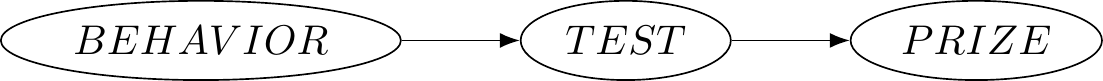
\includegraphics{decisiontheory_files/figure-latex/unnamed-chunk-7-1} \caption[Simple causal pathway]{Simple causal pathway}\label{fig:unnamed-chunk-7}
\end{figure}

Given our assumptions, there is just one way for you to get the prize. You getting the prize depends on you passing the test, and you passing the test depends on you studying. We can express these dependencies using some very simple equations. Let's use `1' to represent cases of studying, passing, and winning the prize, and we'll use `0' to represent partying, failing, and not getting a prize. In addition, we'll read `X:=Y' as `the value of X depends on the value of Y'.\footnote{Note the direction of dependency, which only goes the one way. Think of `:=' as a single symbol, like going backwards along the arrow on the diagrams.} The following single equation then represents that the PRIZE variable depends on the TEST variable:
\[
PRIZE := TEST
\]
and similarily the TEST variable depends on the BEHAVIOR variable:
\[
TEST := BEHAVIOR
\]
Given these equations, we can imagine there are three ways to ensure that PRIZE = 1.\footnote{Heads up: the first two are weirder than the third.} The first, as if by the power of God, is to simply just make PRIZE = 1. This is a bit awkward, for effectively we are `'screening off'' all the upstream causes in the graph as if they didn't really matter after all. The second, which is less arbitrary (given our other assumptions), is to make TEST = 1. By the equation \(PRIZE := TEST\) this makes PRIZE = 1. But this is still not the way that we're thinking about our example, particularly give the way we have drawn our simple graph. The only way to make PRIZE = 1 given what is in our control is to set BEHAVIOR to be 1. This in turn makes TEST = 1 given that \(TEST:= BEHAVIOR\) and then PRIZE = 1 given that \(PRIZE:=TEST\). In the causal modeling literature, all three of these possibilities we've covered would count as a kind of ``intervention'', but what they have in mind is an intervention on the model. What we mean here by `intervention' is being in control of a variable by being able to set its value.

There is, nevertheless, a sense in which getting the prize is in your control, even if you can't directly intervene on that variable. When we set \(BEHAVIOR\) to 1, that fact, combined with the causal graph, will have guaranteed downstream consequences that ultimately make \(PRIZE\) equal to 1.

The simple scenario we have been working with might remind you of decisions made under certainty. Our primary interest, however, has been dealing with decisions where there is some amount of uncertainty, i.e.~where there are some things that are outside of our control that combine with our decision to generate an outcome. For example, suppose you are playing a game where your friend is going to flip a fair coin and you can choose to either bet or not bet while it is in the air. If you bet and the coin lands heads, you win a dollar. If you bet and the coin lands tails, you lose a dollar. And if you choose not to bet at all then you don't win or lose anything. In our standard matrix representation, this scenario looks like this.

\begin{longtable}[]{@{}lcc@{}}
\toprule
& Heads & Tails\tabularnewline
\midrule
\endhead
Bet Heads & \$1 & -\$1\tabularnewline
Don't Bet & \$0 & \$0\tabularnewline
\bottomrule
\end{longtable}

We can use our graphs to also represent this situation. We'll have three nodes, one for the possible actions (bet / don't bet), one for the possible world states (heads / tails), and one for the possible outcomes (the four cells in our table).

\begin{figure}
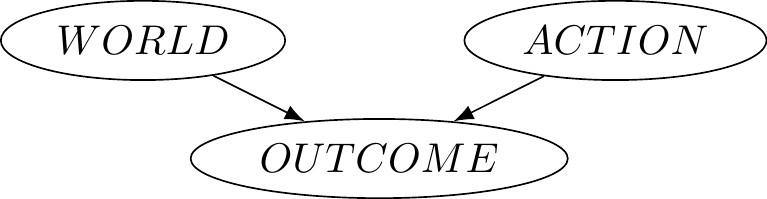
\includegraphics{decisiontheory_files/figure-latex/unnamed-chunk-8-1} \caption[General Causal Pathway for Decisions]{General Causal Pathway for Decisions. The WORLD bubble is like all the columns in our decision tables, the ACTION bubble is like all the rows, and the OUTCOME bubble is like all the cells of a table.}\label{fig:unnamed-chunk-8}
\end{figure}

In addition to this graph, we can write down the equation that will determine how much money you would receive as the outcome. As the graph suggests, this depends on both your action and the world, though you only have control over the former. We'll use `1' to represent that you bet and `0' that you don't, and `1' to represent that the coin turned up heads and `-1' that it did not. The equation is:
\[
OUTCOME := ACTION \times WORLD
\]
Inserting the relevant combinations of values for the actions and world states will output the corresponding values in the outcomes.\footnote{Exercise: What do those values need to be?}

We now have three kinds of representations we can make use of.\footnote{That is, tables, graphs, and some equations.} The graph representation will be particularly helpful for illustrating some important points.\footnote{Don't be fooled by the simplicity of the diagrams. They represent a lot of information.} In general, a causal graph is a collection of nodes with arrows between them. An arrow represents that a node (a variable) has a direct influence on another node (the one that the arrow is pointing to). The node where the arrow starts is called the parent node, and the arrow where the arrow points is the child node. When there is a chain of arrows, a node can have `upstream' ancestors (parents, parents of parents, parents of parents of parents, etc.), as well as `downstream' descendants. Since the arrows are representing causation, and causation only flows in one direction, the collection of arrows cannot have cycles, i.e.~it is never the case that a node can be connected back to itself by following a chain of upstream arrows (nor similarly downstream ones).

\hypertarget{common-causes}{%
\section{Common Causes}\label{common-causes}}

An important concept that causal graphs help us illustrate is the idea of a common cause. Let's suppose that you occassionally suffer from severe headaches. A pretty good indicator of whether you will get one later in the day is if you have ``spots'' in your vision in the morning. You also notice that on days when you eat a banana in the morning you tend not to get a headache later in the day. Let's use \(H=1\) to represent that you get a headache, \(H=0\) that you don't, \(V=1\) that you have spots in your vision, \(V=0\) that you don't, and \(A=1\) that you ate a banana in the morning and \(A=0\) that you didn't. The causal graph would look like this.

\begin{figure}
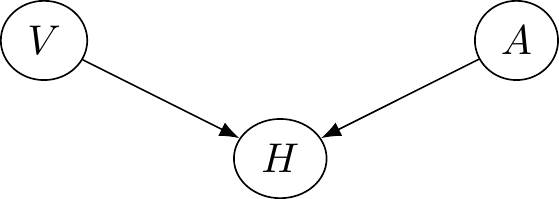
\includegraphics{decisiontheory_files/figure-latex/unnamed-chunk-9-1} \caption[Getting a headache can depend on having spots in your vision or whether you ate a banana]{Getting a headache can depend on having spots in your vision or whether you ate a banana.}\label{fig:unnamed-chunk-9}
\end{figure}

The equation for the value of the headache variable would be:
\[
H:= V\times (1 - A)
\]
It is helpful to see the four relevant possibilities in the form of a table.

\begin{longtable}[]{@{}ccc@{}}
\toprule
\(V\) & \(A\) & \(H:= V\times (1 - A)\)\tabularnewline
\midrule
\endhead
1 & 1 & 0\tabularnewline
1 & 0 & 1\tabularnewline
0 & 1 & 0\tabularnewline
0 & 0 & 0\tabularnewline
\bottomrule
\end{longtable}

When we do some reasoning with these representations, we'll notice that the only time you get a headache is when you have spotty vision but choose not to eat a banana.

Now lets add in an additional consideration. Suppose that you go to the doctor and they note that you are prone to a potassium deficiency. A potassium deficiency, they tell you, can often lead to spots in vision, as well as cravings for bananas (because they are high in potassium!). Suddenly you realize that the days that you had headaches were days when you had both spotty vision in the morning and also had cravings for a banana - but for one reason or another you decided not to eat one. Equipped with this new knowledge, you now make sure you always have bananas on hand so that you can choose to eat one when you have a craving.

Let's update our causal graph. You'll notice that a potassium deficiency has two effects, one on spotty vision and one on your choice to eat a banana. Let's say \(D=1\) means you have a potassium deficiency and \(D=0\) means you don't.

\begin{figure}
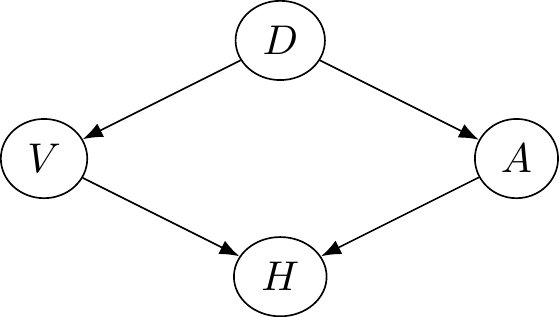
\includegraphics{decisiontheory_files/figure-latex/unnamed-chunk-10-1} \caption[A common cause pathway]{A common cause pathway. A deficiency of potassium causes both spots in vision and a desire to eat bananas.}\label{fig:unnamed-chunk-10}
\end{figure}

This more complicated causal graph can no longer be represented by a single equation. Rather, we now need a \emph{system} of equations that when taken together represent the graph.\footnote{In the literature each line is called a \emph{structural} equation, and the collection of them is the \emph{system} of structural equations.}

\[
\begin{aligned}
V &:= D\\
A &:= D \\
H &:= V\times(1-A)
\end{aligned}
\]

If we now consider the possibilities, we'll notice that you never get a headache. This is because on the days that you would get a headache from spotty vision are days when you have a potassium deficiency, but a potassium deficiency also means that you will eat a banana, and thereby counteract the headache. In our example, spotty vision and eating bananas have a \textbf{common cause}, namely a potassium deficiency.\footnote{Try out this reasoning on the system of equations: set \(D=0\) and find the value of \(H\), then do it again when you set \(D=1\). What do you notice about the value of \(H\) in each case?}

Causal graphs make it really easy to spot when two or more variables have a common cause. We simply take those nodes and trace the upstream arrows: if the variables all have a common ancestor, then they have a common cause (the variable that is the common ancestor).

When two or more variables have a common cause, those variables will be highly correlated with each other, even though they are not causes of one another. For example, an increase in ice cream sales can be correlated with an increase in pool drownings. We should not think, however, that ice cream sales cause pool drownings (nor for that matter, that pool drownings cause more ice cream sales!). Rather, an increase in ice cream sales and pool drownings have a common cause: an increase in temperature, which tends to cause people to both buy more ice cream and to go swimming (which in some cases unfortunately leads to some people drowning).\footnote{Careful here. If \(X\) is a common cause of \(Y\) and \(Z\), then \(Y\) and \(Z\) will be correlated. But just because \(U\) and \(W\) are correlated does not mean they have a common cause - some correlations are \emph{spurious}. See \href{https://www.tylervigen.com/spurious-correlations}{these examples of spurious correlations.}}

Similarly in our case: your spotty vision does not cause you to choose to eat bananas, nor does eating bananas cause your spotty vision. Rather, it is a potassium deficiency that causes both.

\hypertarget{application-to-newcomb-like-problems}{%
\section{Application to Newcomb-like Problems}\label{application-to-newcomb-like-problems}}

Causal models help us gain insight into some of the decision problems we've seen. Recall Newcomb's problem, where a game show host consulted an AI that has profiled you to determine whether to put a million dollars into a second box or not. The payoff table looked like this:

\begin{longtable}[]{@{}lcc@{}}
\toprule
& AI predicts two box & AI predicts one box\tabularnewline
\midrule
\endhead
\textbf{One box (just A)} & \$0 & \$1,000,000\tabularnewline
\textbf{Two box (A and B)} & \$1,000 & \$1,001,000\tabularnewline
\bottomrule
\end{longtable}

What this table hides are causal assumptions about the outcomes. We have been insisting that when we set up decision matrices that the rows are the choices or actions available to us that are in our control, and the columns are the world states - the things that we are uncertain about and are out of our control. Using our simple causal pathway diagram to illustrate this, we might think that the following represents the above table:

\begin{figure}
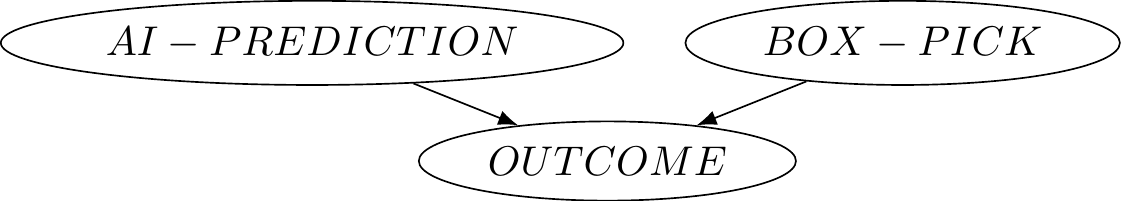
\includegraphics{decisiontheory_files/figure-latex/unnamed-chunk-11-1} \caption[Misleading representation of Newcomb problem]{Misleading representation of Newcomb problem}\label{fig:unnamed-chunk-11}
\end{figure}

But given the narrative of the scenario, there is a correlation between what the AI predicts and what people choose to do. The reason for this correlation is not an accident - after all it is stipulated that the predictions of the AI are highly reliable (even if it's not perfect). When the AI makes a prediction on what someone will choose, it is consulting some body of information that we reasonably could put under the umbrella of a person's \emph{character}. That is, a person's character is a guide to what action they are likely to select (their box pick: one or two) as well as what the AI will predict (which leads to world state: \$1M in box A or not). So a better respresenation of this situation would be the following causal graph:

\begin{figure}
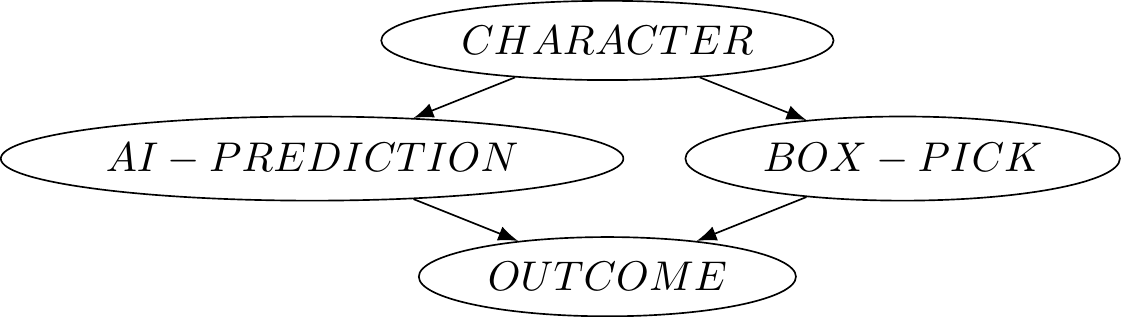
\includegraphics{decisiontheory_files/figure-latex/unnamed-chunk-12-1} \caption[Newcomb pathway]{Newcomb pathway}\label{fig:unnamed-chunk-12}
\end{figure}

This representation makes it clear that there is a common cause to the AI's prediction and your action. If that's right, then the setup is actually not a legitimate kind of decision making problem, since we are not maintaining that the world states and actions be independent of one another. It is not obvious, however, how we might go about fixing this and numerous proposals exist, some of which we'll cover in due course.

First, let's see how some other examples we've discussed are like the Newcomb problem. Consider again the situation where you are deciding whether to work on a project from home or to show up to the park to play a game of frisbee with your friends. In that decision problem, the uncertainty involved whether ``Annoying Guy'' would also show up. Here was the utility table we had.

\begin{longtable}[]{@{}lcc@{}}
\toprule
& Annoying guy stays home & Annoying guy shows up\tabularnewline
\midrule
\endhead
\textbf{You stay home} & 2 & 0\tabularnewline
\textbf{You show up} & 3 & 1\tabularnewline
\bottomrule
\end{longtable}

We additionally suggested that, while you might not like it, you and Annoying Guy are very much alike. In fact, let's just suppose that you and Annoying Guy are identical twins. What this means for this example is that what you choose to do is correlated with what Annoying Guy does. We can again use a causal graph to model this situation. When we do, we need to decide whether the correlation between your choice and Annoying Guy's is completely accidental, or whether there is a reason for that correlation. We have suggested that it's the latter. If we unpack this, it would be again reasonable to think that the correlation reflects a common cause between the two of you: you have similar characters.\footnote{And given that we said you are identical twins, the common character could be the effect of having a common physiology, but we leave that out for now.} So we might have this kind of causal graph:

\begin{figure}
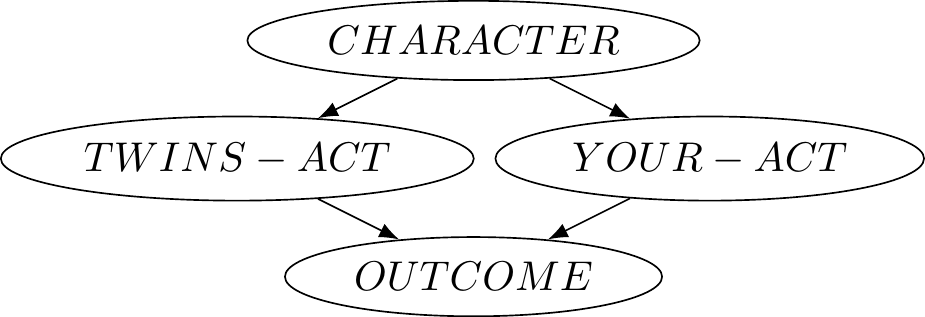
\includegraphics{decisiontheory_files/figure-latex/unnamed-chunk-13-1} \caption[The Twin Example]{The Twin Example}\label{fig:unnamed-chunk-13}
\end{figure}

Think about another example we've discussed about whether to study for a test or to party. Here too it might be tempting to set up a graph that looks like this.

\begin{figure}
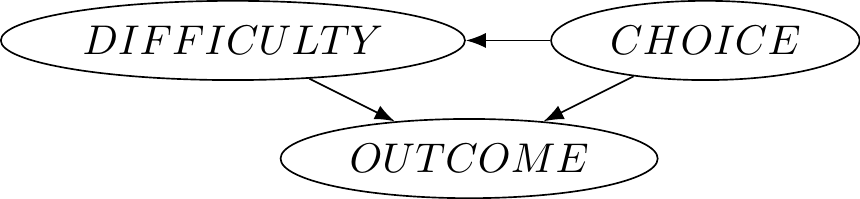
\includegraphics{decisiontheory_files/figure-latex/unnamed-chunk-14-1} \caption[Test Example - Incorrect decision model setup because world states and acts are supposed to be independent, but they are not (CHOICE is a common cause)]{Test Example - Incorrect decision model setup because world states and acts are supposed to be independent, but they are not (CHOICE is a common cause).}\label{fig:unnamed-chunk-14}
\end{figure}

But that graph is incorrect. We insisted that we had to be careful to understand that what it means for a test to be difficult is independent of the action to study - ``difficult'' had to be some kind of measure by which an instructor uses to design questions. This is because your studying for the test can affect the \emph{perceived difficulty} of it, and that would violate our requirement that the world states be independent of the actions. A causal graph makes it clear why we have to be careful: if we're not, then your choice (study or party) would be the common cause of the outcome!

If world states and our choices are independent prior to the outcome, as we are trying to be careful to do, then we should have this:

\begin{figure}
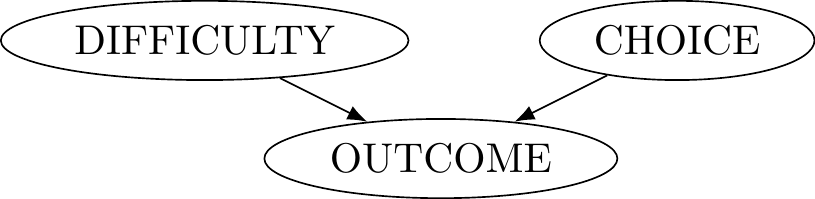
\includegraphics{decisiontheory_files/figure-latex/unnamed-chunk-15-1} \caption[Test Example - Correct decision model setup if we insist that world states and acts are supposed to be independent]{Test Example - Correct decision model setup if we insist that world states and acts are supposed to be independent.}\label{fig:unnamed-chunk-15}
\end{figure}

What we might notice is that the Newcomb problem is more like the incorrect test example if we take into account something like a person's character. Newcomb-like problems all seem to have a kind of causal structure where, if we go back far enough, there are common causes that influence both the world state and our action. That is, if we were to map out causal graphs in more detail, they are likely to end up looking something like the following.

\begin{figure}
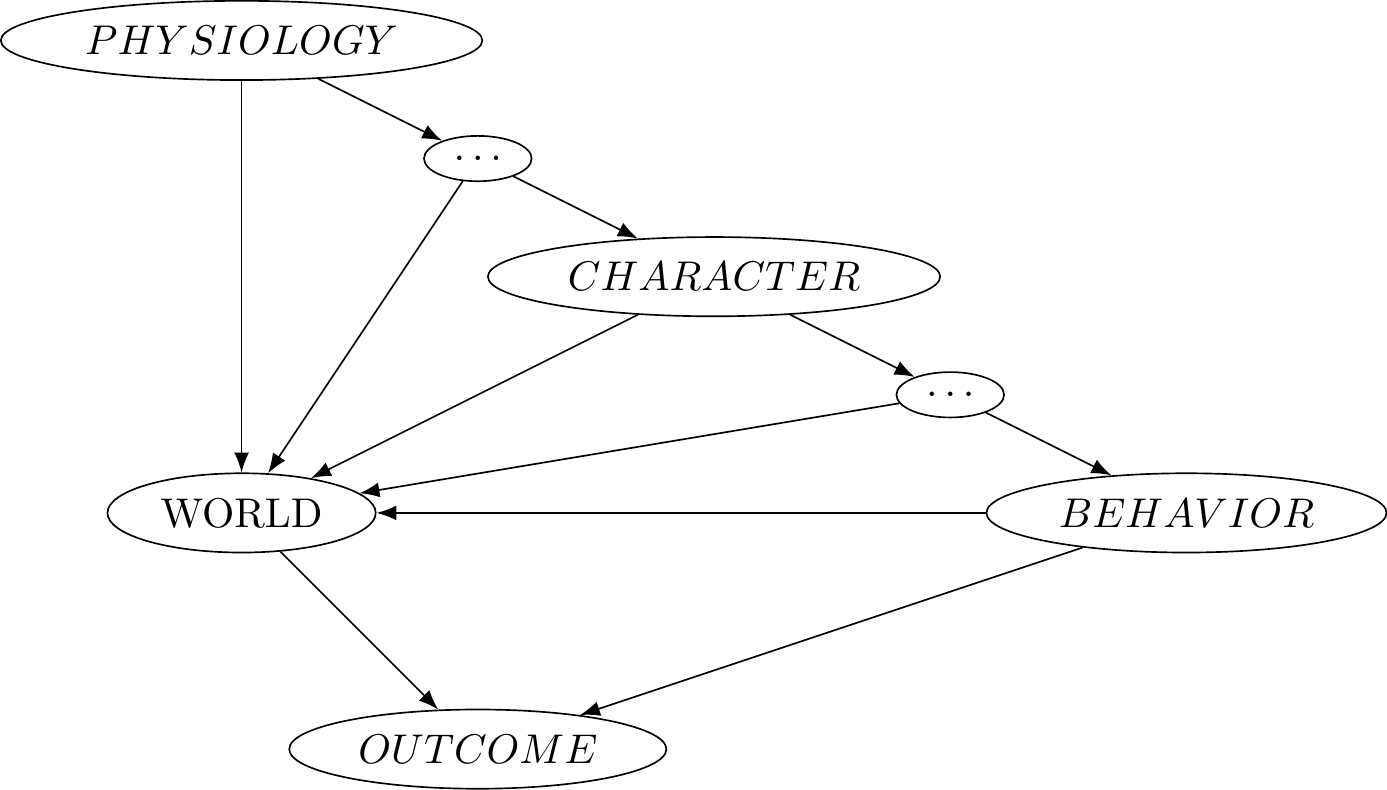
\includegraphics{decisiontheory_files/figure-latex/unnamed-chunk-16-1} \caption[More realistic causal graphs of decisions]{More realistic causal graphs of decisions. The idea to represent things in this way come from Kenny Easwaran's 'A classification of Newcomb problems and decision theories' in *Synthese* (2021, 198).}\label{fig:unnamed-chunk-16}
\end{figure}

What are we to make of these kinds of situations? Isn't it true that our choices can impact several different variables in this chain? Regularly choosing to exercise can impact our physiology - that's the whole point behind training! And in the banana example it can ensure that we don't get a potassium deficiency, and if we do we still can prevent our headaches. And isn't it the case that the way we develop our character is by regularly making the kind of choices that correspond to the kind of person we want to be? In the Newcomb problem, we want to be the kind of person that picks the one box, since that's the kind of information the AI would use to make its prediction, which in turn makes it highly likely that there will be a \$1M in the box! Do these kinds of considerations mean the world state is in a person's control after all?

We have been using the idea of control in a binary (on/off) kind of way, but as the causal graph above suggests, what is and isn't in our control might not be such a clear thing. Perhaps a better way to think of control is that it comes in degrees. Towards the left side of the causal graph are things we have less control over, like our physiology, and towards the right are things that we have more control over, like our behavior in a particular moment.

Whether control is binary or comes in degrees, what we are drawing attention to is a question about where the locus of a choice is. We will see shortly that how one answers this question will largely determine the type of decision theory one ends up endorsing.

\hypertarget{the-locus-of-choice-and-types-of-decision-theories}{%
\section{The Locus of Choice and Types of Decision Theories}\label{the-locus-of-choice-and-types-of-decision-theories}}

It is reasonable to suggest that rationality has a kind of unity. We started our analysis of decision making by defining instrumental rationality - an action is more or less rational depending on how well it helps achieve some goal or aim. Similarly, there is a principle that connects what is possible for us to do and what we ought to do: if something is not in our control to do, then it's false to say that we have an obligation to do it. One way to wrap up some of these considerations is with a kind of ``enkrasia'' principle along the following lines:

\textbf{(Unity of Rationality)} It is rational to do X if and only if: i) it is rational to \emph{plan} to do X, and ii) it is rational to have character traits that lead to planning to do X, and iii) it is rational to have the kind of physiology that allows for the development of such character traits, and so on.

If the unity of rationality is true and we are trying to maximize expected utility, then for Newcomb-like problems we should be selecting the analogs of the one-box option. For if we did not, then selecting the two-box option in the moment is a reflection of our broader character, which means the AI would have made that prediction, and so we would be missing out on \$1M (and consistently so if we went on the game show multiple times).

The dominance argument suggests, however, that the rational thing to do is to pick the two-box option. How can this be rational if that effectively guarantees that one will be consistently missing out on \$1M? There are at least two things to say here. First, one might suggest that the world is imperfect and sometimes it rewards what is irrational. Just because the world rewards the irrational does not detract from the rationality of the choice.\footnote{David Lewis has made this sort of response in his `Causal Decision Theory' in 1981.}

The second thing one could say is that rationality might not have the sort of unity that is suggested above. That is, perhaps in some situations it is possible that the rationality of doing X is at odds with the rationality of planning to do X, or is at odds with the rationality of having the relevant character traits. That is, if we deny the unity of rationality, one might say that it is perfectly consistent to develop a character that corresponds to being a one-box kind of person, but then in the moment on the game show where one makes the choice, one chooses to two-box at the very last minute. The dominance argument seems to be suggesting something along these lines if the outcome of winning \$1M + \$1,000 is a live possibility at all.

A related difficulty concerns about our \emph{knowledge} of what is and is not in our control, as well as our \emph{knowledge} about the kind of character or physiology we have. In fact, it's not unreasonable to think in some cases our brains are planning to do something what we aren't consciously aware of (yet), and so in a sense we might not have knowledge of our own plans. How might that affect our considerations about the unity of rationality? Let's illustrate with an example.

There is a parasite called \emph{toxoplasma gondii} that is primarily hosted by cats but affects mammals in general. Infected individuals tend not to show symptoms, but there do exist a wide range of negative effects. Interestingly, infected rats will tend to be less afraid of cats and even be attracted to cat urine, which from the parasite's perspective is advantageous because that's how it perpetuates its life-cycle (the larvae develop in rats and then mature in cats, laying more eggs in the excrement of cats which are then picked up by rats).

Consider then an agent that knows it's possible they have toxoplasmosis. Given this possibility, they know that there is some chance that they will experience negative effects from it, but they also know that they are more inclined to adore cats by, e.g., speaking to them, collecting pictures of them, and potentially even petting them. That is, they consider the following causal graph.

\begin{figure}
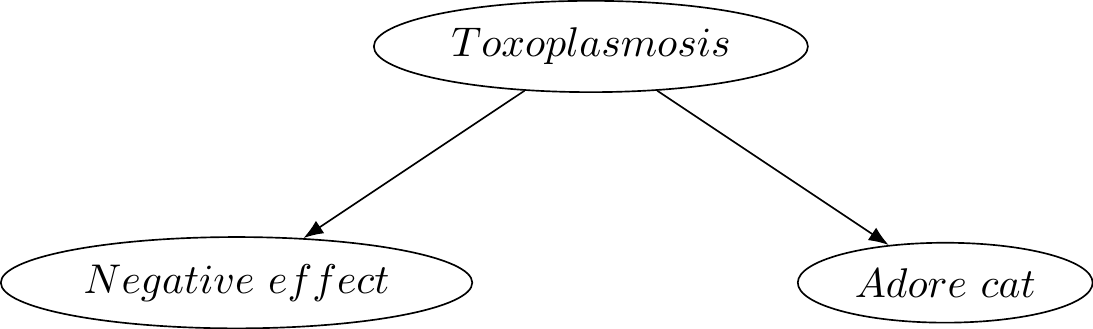
\includegraphics{decisiontheory_files/figure-latex/unnamed-chunk-17-1} \caption[Toxoplasmosis problem]{Toxoplasmosis problem}\label{fig:unnamed-chunk-17}
\end{figure}

Let's assume that while the chances of negative side effects are small, the negative utilities of those side effects are very large, whereas the utilities that come with adoring cats is relatively small in comparison. Should the agent decide to adore cats or not?

If the agent uses the causal graph as is, they might reason that choosing to adore cats is itself evidence of having toxoplasmosis, which in turn makes it more likely that they will have negative effects. Note that their choice \emph{does not cause} the negative effects. Rather, when they consider the action of adoring cats, they in turn use that as new information about themselves! And that in turn might influence what they end up deciding to do. We don't yet have the machinery from probability theory to make this more precise, but know that so long as the negative utilities are sufficiently larger than the positive utilities, and the probabilities for negative effects aren't too small, the agent will choose not to adore cats.

Alternatively, the agent might follow our insistence that there be no common causes between the world states and our relevant choices. So to the extent that they have a choice in adoring cats or not, this will be independent of the already settled fact of whether they have toxoplasmosis or not. To represent this, they modify the causal graph so that they severe the dependence arrow from toxoplasmosis to adoring cats:

\begin{figure}
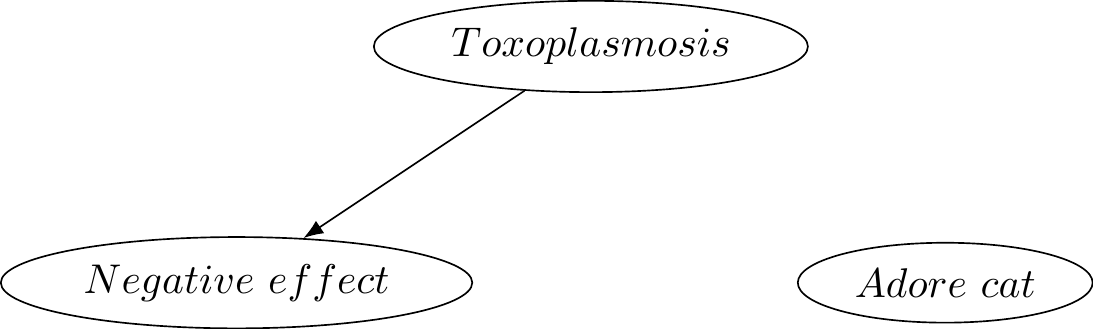
\includegraphics{decisiontheory_files/figure-latex/unnamed-chunk-18-1} \caption[Toxoplasmosis problem - intervened]{Toxoplasmosis problem - intervened.}\label{fig:unnamed-chunk-18}
\end{figure}

In this way of reasoning, the agent recognizes that adoring cats is evidence that they have toxoplasmosis, but this is already accounted for in the other two nodes and the connection between them. In this reasoning, toxoplosmosis does not cause the \emph{choice} of adoring cats. So now when they reason about what to do, they recognize that adoring cats always adds some small extra utility (say 1), regardless of whether the world state is that they have toxoplasmosis or not (where toxoplasmosis has a negative utility of 1000, say).

\begin{longtable}[]{@{}lcc@{}}
\toprule
& Has toxoplasmosis & Does not\tabularnewline
\midrule
\endhead
\textbf{Ignore cats} & -1000 & 0\tabularnewline
\textbf{Adore cats } & -1000 + 1 & 0 + 1\tabularnewline
\bottomrule
\end{longtable}

From this perspective, the agent reasons that they should adore cats, since that's the dominant option.

What we are illustrating with this last example is a question about whether choices, wherever they are located in the causal graphs, can be informative about the very causal graphs we are using to guide our choices.

So we have two kinds of questions. One kind of question is about \newthought{ where the locus of choice is}. The other kind of question is about \newthought{whether interventions related to choices are further evidence} to be used in our reasoning. It turns out that how we answer these questions will characterize different kinds of decision theories.

The most common decision theory, called \newthought{causal decision theory} (CDT), puts the locus of choice furthest to the right of the causal graph we had above, i.e., a choice for the purpose of standard decision making is what decides the behavior. Variables that are upstream, such as character and physiology, are not part of what is being analyzed, at least not for the purpose of understanding rationality in terms of comparison of options.

On the other extreme of the causal graph, and a more recent addition to the literature, is \newthought{functional decision theory} (earlier known as \textbf{timeless decision theory}). On this decision theory options are compared by considering the furthest upstream points of evaluation. So if that happens to be character, for example, then options are compared by imagining the impacts of interventions (the removal of causal arrows) at those points. In some presentations of FDT, we imagine that we are choosing what kind of robot or set of functions we do best in a decision problem.

A third kind is \newthought{evidential decision theory} (EDT). The idea behind EDT is that we don't intervene on a causal graph at all when we analyze what to do. Rather, just like in the toxoplasmosis example, we simply conditionalize on the evidence that is captured on the graph. This notion of conditionalization has a technical meaning that is addressed in probability theory. So it is finally time for us to get clear on what we mean when we talk about probabilities.

\hypertarget{exercises-6}{%
\section*{Exercises}\label{exercises-6}}
\addcontentsline{toc}{section}{Exercises}

\begin{enumerate}
\def\labelenumi{\arabic{enumi}.}
\item
  Consider the following system of structured equations: \[\begin{aligned}
  O &:= W \times A\\
  A &:= P \\
  W &:= C \\
  P &:= C \\
  \end{aligned}
  \]
  Draw the corresponding causal graph.
\item
  Here is an example to consider from Derek Parfit (1984): Suppose that I am driving at midnight through some desert. My car breaks down. You are a stranger and the only other driver near. I manage to stop you, and I offer you a great reward if you rescue me. I cannot reward you now, but I promise to do so when we reach my home. Suppose next that I am transparent, unable to deceive others. I cannot lie convincingly. Either a blush, or my tone of voice, always gives me away. I want to get the major benefit of a ride out of the desert, but actually giving you the reward is a cost to me. So ideally, I would like to be able to formulate a sincere plan to give you the reward, a plan that is sufficiently sincere that you come to believe me and give me a ride out of the desert, but after having gotten the ride I'd rather not follow through on this plan.

  \begin{itemize}
  \tightlist
  \item
    Using the causal graph model representation, analyze this decision (note that planning happens somewhere between CHARACTER and BEHAVIOR). You may find it helpful to also include the decision table like we have been doing.
  \end{itemize}
\item
  Here is an example from Egan (2007): Paul is debating whether to press the ``kill all psychopaths'' button. It would, he thinks, be much better to line in a world with no psychopaths. Unfortunately, Paul is quite confident that only a psychopath would press such a button. Paul very strongly prefers living in a world \emph{with} psychopaths to dying.

  \begin{itemize}
  \tightlist
  \item
    Represent Paul's decision problem in a standard decision matrix. Then draw a causal graph diagram for it. Is there a common cause here? This is sometimes presented as a problem for causal decision theory. Explain how that could be.
  \end{itemize}
\item
  In our discussion of the unity of rationality, we considered the possibility that an action is rational even though ``the world'' would reward the irrational action (at least according to dominance reasoning). Can you think of any examples besides our discussion of the Newcomb Problem or the Toxoplasmosis Problem? What argument would support the claim that the example action is rational despite the world rewarding a different action (is it the dominance strategy or something else)?
\end{enumerate}

\hypertarget{odds-probabilities-and-actions}{%
\chapter{Odds, Probabilities and Actions}\label{odds-probabilities-and-actions}}

We have come to the point where it will no longer be enough to work with our intuitive notion of probability. If we want to go beyond toy decision problems, like the one's we've been covered, and model decisions that are more like the ones we more frequently face, we'll need to have a sufficiently robust understanding of probability. For example, one of the main things we'll want to be able to do is update our beliefs given new information, which effectively amounts to knowing how to update probabilities.

Probabilities are a way of quantifying beliefs. It may seem impossible to measure something as elusive and subjective as beliefs. But some clever conceptual tools have been developed to do just that.

\newthought{The key idea behind measuring a person's belief} about the world is to figure out how willing they are to risk things that they care about. To illustrate this idea we're going to momentarily assume that money is our measure of utility.

\hypertarget{odds-and-fair-betting-rates}{%
\section{Odds and Fair Betting Rates}\label{odds-and-fair-betting-rates}}

Here's a roughly general observation of people's behaviour: the more confident someone is that some event is going to happen, the more willing they are to bet.

Suppose \(S\) is some event that Bob and Ally care about. The event might be a sports team winning a game, that it's going to rain tomorrow, that the stock price of some company will be higher by next year, etc.

Let's say Bob is more than 50\% confident that \(S\) will happen. In fact, let's suppose that Bob would accept a deal that would pay him \(\$1\) if \(S\) happens, but would cost him \(\$2\) if it doesn't. Let's say Ally thinks Bob is wrong to be so confident and agrees to take Bob's bet. In effect, this means that Ally is willing to put \(\$1\) on the table for the chance of winning the \(\$2\) that Bob is willing to put on the table. The \textbf{stake} is the sum of all the money on the table, in this case \(\$1 + \$2 = \$3\). Whoever ends up being right gets to take the stake.\footnote{Careful here. If Ally turns out to win because \(S\) does not happen, she wins the stake (\(\$3\)), but since she contributed \(\$1\) to it the amount she \emph{gains} is \(\$2\).}

\newthought{Bob's fair betting rate} can be expressed by dividing his potential loss by the stake:

\[
  \begin{aligned}
    \mbox{Betting Rate} &= \frac{\mbox{Potential Loss}}{\mbox{Stake}}\\
                        &= \frac{\$2}{\$2 + \$1}\\
                        &= \frac{2}{3}.
  \end{aligned}
\]

Bob's betting rate is \(2/3\), which is a reflection of how confident he is that \(S\) will happen. And here's the next move: that's Bob's personal probability that \(S\) will happen, i.e.~\(Pr_{Bob}(S)=2/3\).

\newthought{Bob's fair odds} is another way that betting is sometimes talked about. To express Bob's fair better rate in terms of odds, we take the ratio of potential loss to potential win:

\[
  \begin{aligned}
    \mbox{Odds} &= \mbox{Potential Loss : Potential Win}\\
                &=  2:1
  \end{aligned}
\]

The odds that Bob would accept are another reflection of his degree of confidence. In fact, there is a handy way of linking up our notion of expected value with odds and probabilities.

\newthought{A fair bet} is one in which the \emph{expected value} is zero. That is, if we weight the potential win by the probability of winning, and we weight the potential loss by the probability of losing, the odds should ``cancel out'': \[ (2/3)(\$1) + (1/3)(-\$2) = 0. \]

Here's a helpful visual way of understanding the idea of ``canceling out''. Notice first an inverse relationship between probabilities and payoffs when it comes to risks (especially in gambling): events with really high payoffs tend to have low probabilities, and likewise, the more probable an event is the lower the payoffs tend to be. If the amount of probability is like the width of a rectangle, and the payoff (or loss) is like the height of a rectangle, then a fair bet will be one in which the area of a rectangle that represents Bob winning will have the same amount of area that represents Bob lossing.

\begin{figure}
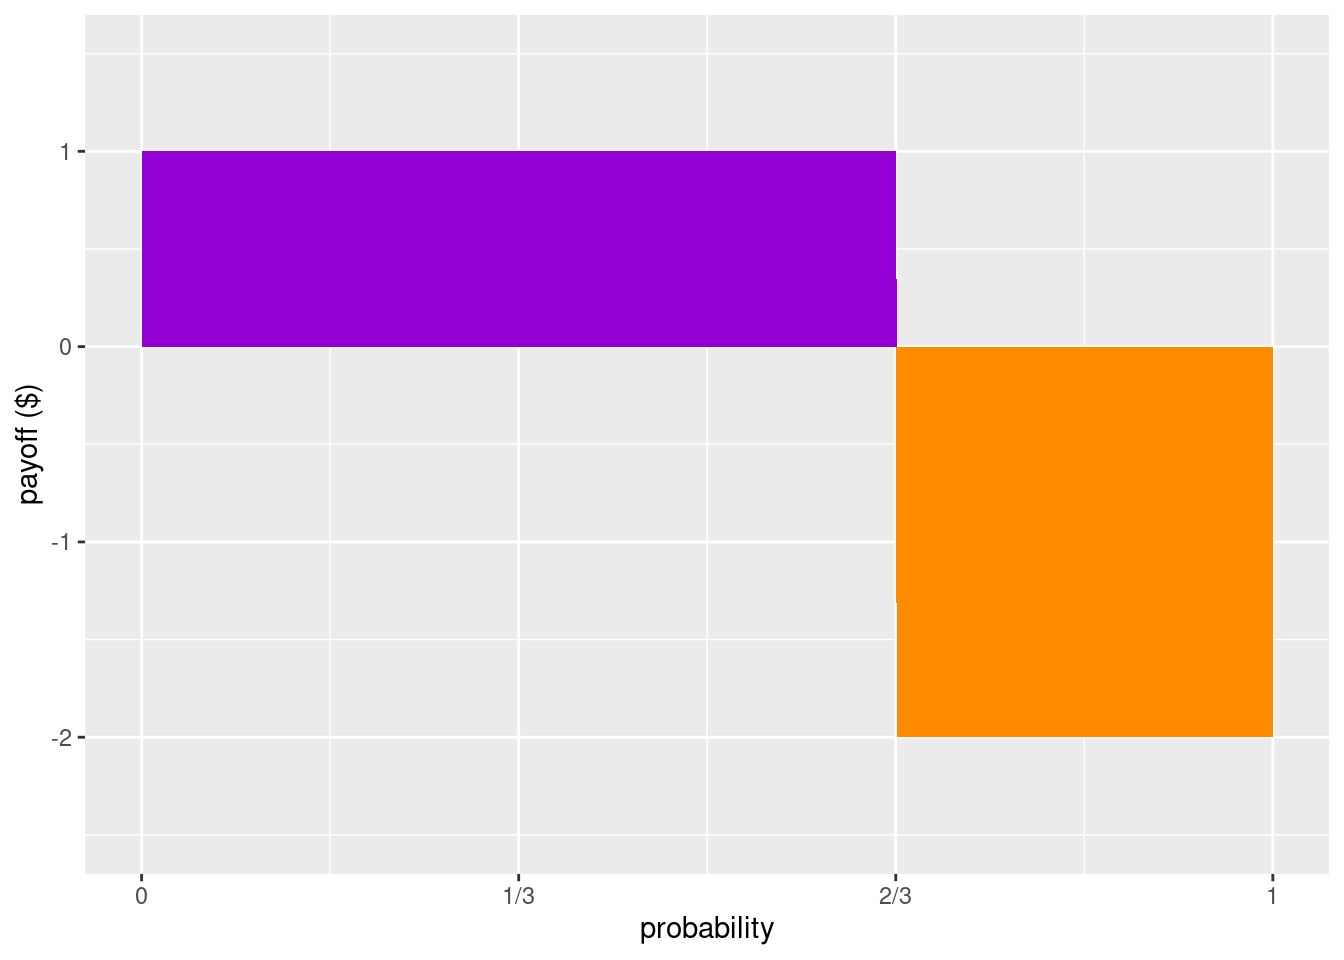
\includegraphics{decisiontheory_files/figure-latex/unnamed-chunk-19-1} \caption[A bet that pays $\$1$ if Bob wins and costs $\$2$ if he loses, is fair when the purple and orange regions have equal area]{A bet that pays $\$1$ if Bob wins and costs $\$2$ if he loses, is fair when the purple and orange regions have equal area: when the probability of winning is $2/3$.}\label{fig:unnamed-chunk-19}
\end{figure}

To be clear, what Bob considers to be a fair bet might change. For example, suppose Bob comes into some information that significantly decreases his confidence that \(S\) will happen. Let's say his confidence goes all the way down to 10\% (i.e.~1/10). Since his confidence went down, he should be willing to risk less, that is, he should be willing to stake much less. How much less? As a fair bet, Bob will want to make sure that the expected value will be 0: \[ (1/10)(\$9) + (9/10)(-\$1) = 0. \] So for Bob to be willing make a bet with Ally give this new information, Ally would need to be willing to put at least \(\$9\) in the stake for Bob's \(\$1\).

Notice how our visualization using rectangles will change for this new scenario, but the two rectangles will still have the same area.

\begin{figure}
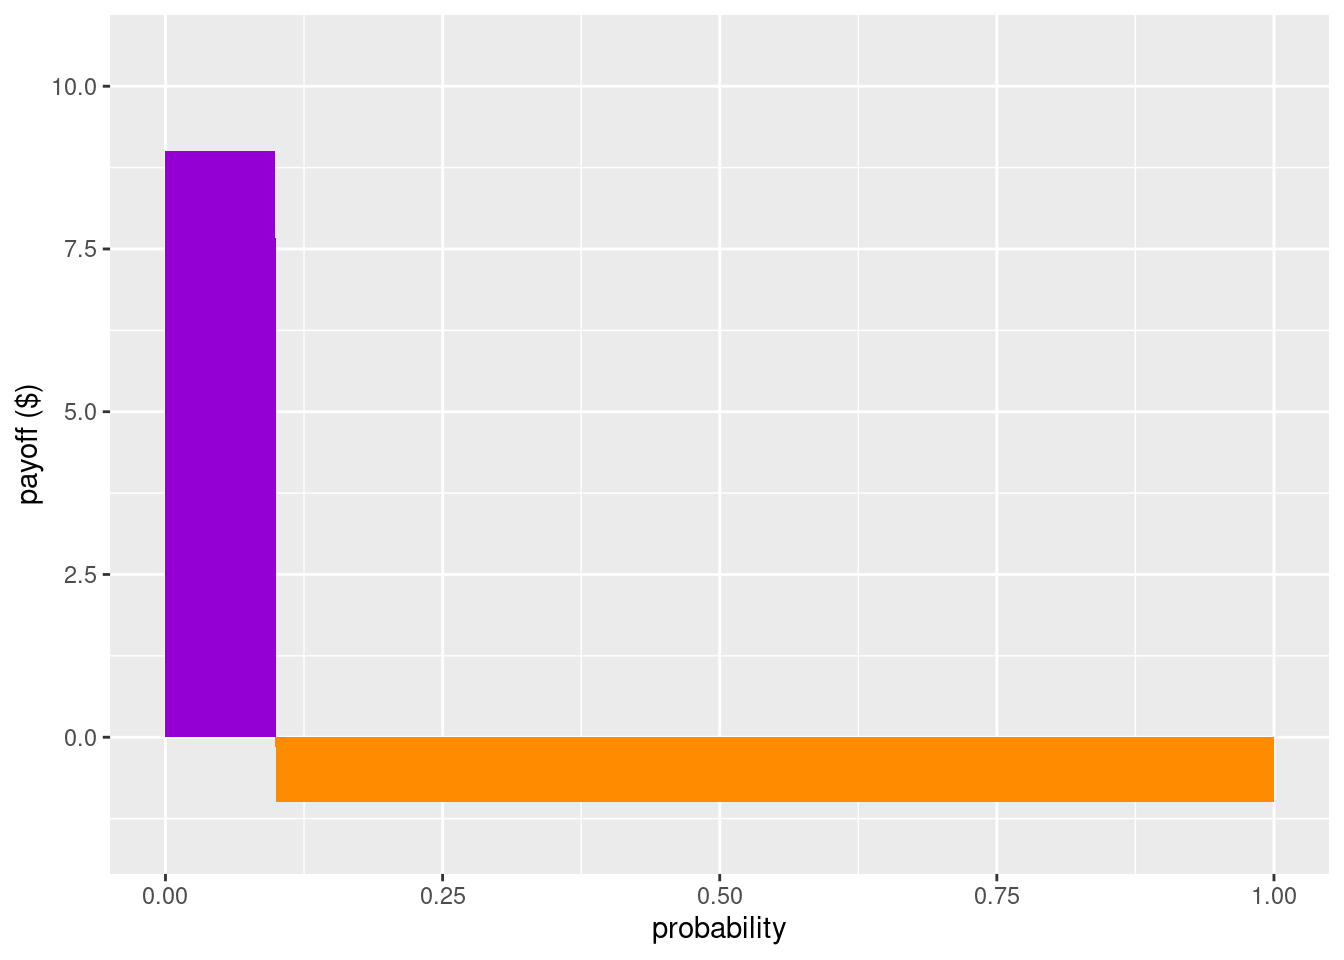
\includegraphics{decisiontheory_files/figure-latex/unnamed-chunk-20-1} \caption[A bet that pays $\$9$ if Bob wins and costs $\$1$ if he loses is fair when the probability of winning is $1/10$]{A bet that pays $\$9$ if Bob wins and costs $\$1$ if he loses is fair when the probability of winning is $1/10$.}\label{fig:unnamed-chunk-20}
\end{figure}

\newthought{Here's a General Recipe} for quantifying a person's probability that a proposition \(S\) is true using the idea of fair bets:

\begin{enumerate}
\def\labelenumi{\arabic{enumi}.}
\tightlist
\item
  Find a bet on \(S\) that they see as fair. Call the potential winnings \(W\) and the potential losses \(L\).
\item
  Because the bet is fair to their eyes, set the expected value of the bet equal to zero:
  \[ [Pr(S) \times W] + [(1-\Pr(S)) \times -L] = 0. \]
\item
  Now solve for \(Pr(S)\):
  \[
     \begin{aligned}
       (Pr(S) \times W)  + ((1-Pr(S)) \times -L) &= 0 \\
       (Pr(S) \times W)  + (-L) + (Pr(S) \times L) &= 0 \\
            (Pr(S) \times W) + (Pr(S) \times L) &= L \\
            Pr(S)\times (W + L) &= L \\
                                      Pr(S) &= \frac{L}{W+L}.
     \end{aligned}
   \]
  Notice that we have the formula for the fair betting rate again! It's helpful to memorize this formula so you don't have to do the derivation each time. But more important than that is knowing that there is a recipe for getting from bets to personal probabilities.
\end{enumerate}

\hypertarget{advantageous-bets}{%
\section{Advantageous Bets}\label{advantageous-bets}}

The general recipe we just developed uses the idea of fair bets (or fair odds). The idea here is that a person would be willing to take either side of the bet. Using the language of preferences: the person is \emph{indifferent} between the two sides. What happens if betting rates aren't fair in the eyes of Bob? In that case Bob would no longer be indifferent, he would want to take one side.

complications with utilities

?show some bets that aren't worth taking to illustrate what's coming in the more technical chapter next?

\hypertarget{probabilities-and-logic}{%
\chapter{Probabilities and Logic}\label{probabilities-and-logic}}

In this chapter we're going to learn what it means when we say that a probability function is a \emph{normalized measure over a possibility space}. There are three parts here: i) what is it for a function to be a measure, ii) what is a normalized measure, and iii) what is a possibility space.

\hypertarget{measures}{%
\section{Measures}\label{measures}}

A function is a mapping from an input to an output. There can be many inputs that are mapped to one output, but to be a function the mapping cannot assign more than one output to an input. We typically think of functions as having numbers as inputs and outputs, but that doesn't have to be the case. In fact, as we'll see, probability functions will have a number as an output, but have non-numbers as inputs.

Consider Scotland. Scotland is known for its whisky. There are six regions (depending on who you ask) where whisky is distilled.

We can represent functions with tables. Let's suppose we have a function that takes distilling regions of Scotland as input and the number of distilleries as output.

\begin{longtable}[]{@{}cc@{}}
\toprule
Input & Output\tabularnewline
\midrule
\endhead
Highlands & 27\tabularnewline
Speyside & 62\tabularnewline
Lowlands & 3\tabularnewline
Campbeltown & 3\tabularnewline
Islay & 8\tabularnewline
Islands & 7\tabularnewline
\bottomrule
\end{longtable}

Notice that there are two inputs that get mapped onto the same output (Lowlands and Campbeltown both have 3 as their output), but no input has any more or less than one output (e.g., it's not the case that Islay has both 8 and 7 distilleries).

\newthought{What it means for a function to be a measure}. \textbf{First}, the function has to have non-negative numbers as output. Our example meets this condition. \textbf{Second}, the input is some space that can have `regions' or subsets. For example, we can organize our distilling regions into those that are on the mainland (the first four in our table) and those not on the mainland (i.e., Islay and Islands). Alternatively, we could group the list into those whose name starts with one of the first ten letters of the alphabet, those that start with `S', and then the rest. The specifics here don't matter, just that different subsets are possible.

\textbf{Third}, and this important property is called \emph{additivity}, is that the measure of a subset is the sum of the measures of the members that make up the subset. For example, suppose we're considering the mainland distillery regions (the first four on our list). Then the number of distilleries on the mainland is just the sum of the distilleries in the regions of Highlands, Speyside, Lowlands, and Campbeltown (95).

It doesn't really matter how we decide to group things. We could decide that the `groups' are just the members themselves. In that case, there is just one number to consider. Or we could consider the entire input as the subset (here `subset' doesn't indicate a strictly smaller set - in set theoretic speak, we say that a set is a subset of itself). For example, the number of distilleries in Scotland is, according to our table, 110 (i.e., the sum of each region).

Not all functions are measures. That is, \emph{some functions fail to be additive}. For example, let's suppose we have a function from distilling regions to the proportion of distilleries owned by multinational companies (these numbers are not necessarily accurate).

\begin{longtable}[]{@{}cr@{}}
\toprule
Input & Output (proportion of owned by corps.)\tabularnewline
\midrule
\endhead
Highlands & 0.6\tabularnewline
Speyside & 0.4\tabularnewline
Lowlands & 0.3\tabularnewline
Campbeltown & 0\tabularnewline
Islay & 0.25\tabularnewline
Islands & 0.4\tabularnewline
\bottomrule
\end{longtable}

Now let's say we want to ask what proportion of the mainland distilleries are owned by multinational companies. We can't do this just by looking at the table above. Adding up proportions won't work: it would lead to the absurd result that the proportion of mainland distilleries owned by international companies is 1.3, that is, 130\%. But it's impossible to own more than 100\% of the mainland distilleries, not to mention own more than 100\% of anything! In general, proportions do not meet the Additivity property and thus cannot serve as the basis for measures. Typical examples of measures include length, area, and volume.

\hypertarget{normalized-measures}{%
\section{Normalized Measures}\label{normalized-measures}}

The `universe' of a function is the entire collection of inputs. In our whisky example above, the universe of our function is the set of distillery regions in Scotland. We could have defined the universe of our function differently. For example, we might have a different function whose universe is the set of countries that have distilleries, including Scotland, Ireland, the United States, Canada, Japan, etc. Also, the universe of a function doesn't have to correspond to physical space. We could have a function with a universe of taste characteristics, like sweet, smoky, earthy, rich, peppery, floral, etc. These are not located in space like distilleries, but are rather properties of how a whisky is perceived by taste.

A \emph{normalized} measure function is a measure function that gives a value of 1 to its universe. By doing so, the measure of every subset can be understood as a proportion of the universe of the function. Any measure can be `normalized' by dividing the value of each output by the value of the whole universe. For example, we can normalize the function represented in the table below by dividing each output number by the sum of all outputs (110). That would give us the normalized values in the following table (rounded to four decimal places).

\begin{longtable}[]{@{}ccc@{}}
\toprule
Input & Output & Normalized\tabularnewline
\midrule
\endhead
Highlands & 27 & 0.2455\tabularnewline
Speyside & 62 & 0.5636\tabularnewline
Lowlands & 3 & 0.0273\tabularnewline
Campbeltown & 3 & 0.0273\tabularnewline
Islay & 8 & 0.0727\tabularnewline
Islands & 7 & 0.0636\tabularnewline
\bottomrule
\end{longtable}

Notice that this normalized function satisfies the property of being additive. We can use the table to answer the question of what proportion of all distilleries in Scotland are on the mainland by adding up the normalized values (keeping in mind that we will need to correct for errors from having rounded the values). This works because the sum of all the normalized values add up to 1. This is unlike the function represented in the previous table where the proportions do not sum to 1.

Normalizing is an important step in taking data from the world and turning it into probability functions. Sometimes the universe of a function is not very well defined. In that case, it will not be possible to normalize. So one important lesson for interpreting results of some data is to understand what the relevant universe is supposed to be.

\hypertarget{possibilities-and-truth-tables}{%
\section{Possibilities and Truth Tables}\label{possibilities-and-truth-tables}}

Let's look at how to build a probability function. We'll start with a really simple example. Suppose we have a fair coin and you're going to flip it twice. In the first flip there are two possible outcomes: heads (H) or tails (T). In the second flip there are again two possible outcomes: H or T. For two flips of the coin then, there are a total of four possible outcomes: HH, TH, HT, TT. We can keep track of these in a table.

\begin{longtable}[]{@{}lcc@{}}
\toprule
& Flip 1 & Flip 2\tabularnewline
\midrule
\endhead
Outcome 1 & H & H\tabularnewline
Outcome 2 & T & H\tabularnewline
Outcome 3 & H & T\tabularnewline
Outcome 4 & T & T\tabularnewline
\bottomrule
\end{longtable}

If we were to flip the coin a third time, we would have 8 possible outcomes, which we can also collect in a table

\begin{longtable}[]{@{}lccc@{}}
\toprule
& Flip 1 & Flip 2 & Flip 3\tabularnewline
\midrule
\endhead
Outcome 1 & H & H & H\tabularnewline
Outcome 2 & T & H & H\tabularnewline
Outcome 3 & H & T & H\tabularnewline
Outcome 4 & T & T & H\tabularnewline
Outcome 5 & H & H & T\tabularnewline
Outcome 6 & T & H & T\tabularnewline
Outcome 7 & H & T & T\tabularnewline
Outcome 8 & T & T & T\tabularnewline
\bottomrule
\end{longtable}

If we were to flip the coin four times, there would 16 possibilities. Each time we add an additional flip, the number of possibilities doubles in total. That is, where \(n\) is the number of coin flips, the total number of possible outcomes is \(2^n\).

Although this example is simple, it turns out to be a really fruitful way of modeling lots of other examples that have the same structure. For example, philosophers love logic and thinking about the world in terms of statements or propositions that are either true or false. Suppose we have three different propositions: P, Q, and R.

\begin{itemize}
\tightlist
\item
  P - "Bert drinks beer on Fridays.''
\item
  Q - "Bert drinks wine on Fridays.''
\item
  R - "Bert drinks Scotch whisky on Fridays.''
\end{itemize}

For simplicity, let's assume that P is true if on the majority of Fridays I have a beer, and is false otherwise. Similarly for Q and R. In the real world each of these propositions has a unique truth value. Our interest here, however, is not just what is true, but the space of possibilities. In this case, each proposition has the possibility of being true (T) or false (F). Following the coin flip example, there are in total eight possibilities. We can organize the possibilities in what logicians call a truth table.

\begin{longtable}[]{@{}lccc@{}}
\toprule
& P & Q & R\tabularnewline
\midrule
\endhead
& F & F & F\tabularnewline
& T & F & F\tabularnewline
& F & T & F\tabularnewline
& T & T & F\tabularnewline
& F & F & T\tabularnewline
& T & F & T\tabularnewline
& F & T & T\tabularnewline
& T & T & T\tabularnewline
\bottomrule
\end{longtable}

These eight possibilities provide the foundation for creating a probability function. What we first need to do is make sure that we have a measure. Let's say we give the following numbers to each row in the truth table. Where the numbers come from is not important to illustrate the point. But we can imagine, at least roughly speaking, that the universe of the function is all Fridays, and the outputs represent the fraction of times I reported what I had to drink. Notice that if we sum up the output values, we get 1. So, we have a measure, and it's a normalized measure.

\begin{longtable}[]{@{}cccl@{}}
\toprule
Probability & P & Q & R\tabularnewline
\midrule
\endhead
0.0002 & F & F & F\tabularnewline
0.001 & T & F & F\tabularnewline
0.0008 & F & T & F\tabularnewline
0.008 & T & T & F\tabularnewline
0.08 & F & F & T\tabularnewline
0.1 & T & F & T\tabularnewline
0.01 & F & T & T\tabularnewline
0.8 & T & T & T\tabularnewline
\bottomrule
\end{longtable}

We can now use this table to ask questions about the probability that a proposition is true. To do that, we look at all the rows where the proposition in question is true, and then add up the output values. For example, suppose we are interested in the probability that P is true (i.e., the probability that Bert drinks beer on a Friday). Notice that P is true in rows 2, 4, 6, and 8. So we would compute \(0.001+0.008+0.1+0.8\) which is 0.909. That is, there is a 90.9\% that Bert drinks beer on a Friday.

We aren't limited to asking the probabilities that a single proposition is true. Sometimes we'll want to ask what the probability is that both P and R is true, or that either P or R is true, or that P is false. These are all examples of more complex sentences. Logicians have a way of expressing these types of complex sentences. They call them conjunctions, disjunctions, and negations, respectively. There are some handy symbols used too:

`P\(\wedge\)Q' means `P and Q' (also called conjunction)
`P\(\vee\)Q' means `P or Q' (also called disjunction)
`\(\neg\)P' means `not P' (also called negation)

What's really handy about these formulations is that the truth values of the complex sentences can be fixed by the truth values of the components. For example, the rule for conjunction is

\begin{longtable}[]{@{}rcc@{}}
\toprule
P & Q & P\(\wedge\)Q\tabularnewline
\midrule
\endhead
T & T & T\tabularnewline
T & F & F\tabularnewline
F & T & F\tabularnewline
F & F & F\tabularnewline
\bottomrule
\end{longtable}

As you may guess, the truth table for negation is pretty simple. The truth value is simply reversed.

\begin{longtable}[]{@{}rl@{}}
\toprule
P & \(\neg\)P\tabularnewline
\midrule
\endhead
T & F\tabularnewline
F & T\tabularnewline
\bottomrule
\end{longtable}

For disjunction the truth value of the whole sentence is given by the following table.

\begin{longtable}[]{@{}ccc@{}}
\toprule
P & Q & P\(\vee\)Q\tabularnewline
\midrule
\endhead
T & T & T\tabularnewline
T & F & T\tabularnewline
F & T & T\tabularnewline
F & F & F\tabularnewline
\bottomrule
\end{longtable}

Notice that this is an inclusive interpretation of `or' which means that disjunction assumes by default that when both component sentences are true then the whole sentence is true. For example, if you are asked, ``Do you want ketchup or mustard on your burger'' there's nothing contradictory about saying that you want both. It's easy enough to express the exclusive version `or' by say something like `P or Q, and not both'. Formally we would write `(P\(\vee\)Q) \(\wedge\) \(\neg\)(P\(\wedge\)Q)'.

We can use the truth table definitions of conjunction, disjunction, and negation to determine the possible truth values of a complex sentence. Consider for example the sentence `(P\(\vee\)R) \(\wedge\) \(\neg\)Q' which can be interpreted as ``On Fridays Bert drinks beer or he drinks Scotch whisky, but he doesn't drink wine.'' (Note that''but'' expresses "and'' with the addition of some flare to highlight a contrast.) Using the rules for \(\wedge\), \(\vee\), and \(\neg\) we get the table below. Notice that the whole complex sentence is a conjunction, where the left conjunct is made out of a disjunction (P\(\vee\)R), and the right conjunct is made out of a negation (\(\neg\)Q). So we have to work from the smallest parts up to the larger parts, which means that we first evaluate `(P\(\vee\)R)', then we evaluate `\(\neg\)Q', and then we can do the column of truth values under `\(\wedge\)' (which have been boldfaced to indicate these truth values are under the main connective).

\begin{longtable}[]{@{}ccccc@{}}
\toprule
Probability & P & Q & R & (P\(\vee\)R) \(\wedge\) \(\neg\)Q\tabularnewline
\midrule
\endhead
0.0002 & F & F & F & F \(~~\) \textbf{F} T\tabularnewline
0.001 & T & F & F & T \(~~\) \textbf{T} T\tabularnewline
0.0008 & F & T & F & F \(~~\) \textbf{F} F\tabularnewline
0.008 & T & T & F & T \(~~\) \textbf{F} F\tabularnewline
0.08 & F & F & T & T \(~~\) \textbf{T} T\tabularnewline
0.1 & T & F & T & T \(~~\) \textbf{T} T\tabularnewline
0.01 & F & T & T & T \(~~\) \textbf{F} F\tabularnewline
0.8 & T & T & T & T \(~~\) \textbf{F} F\tabularnewline
\bottomrule
\end{longtable}

Notice that the complex sentence is true on rows 2, 5, and 6. So as an example, if P is true but Q and R are false, then P\(\vee\)R) \(\wedge\) \(\neg\)Q is true (this is row two).

If we want to calculate what the probability is that `(P\(\vee\)R) \(\wedge\) \(\neg\)Q' is true, all we need to do is add up the probabilities that correspond to each row. This would be \(0.001+0.08+0.1 = 0.181\). That is, there is an 18.1\% chance that on Fridays Bert drinks beer or Scotch whisky, but doesn't drink wine.

It is worth pointing out several features about probabilities that correspond to some important logical concepts: tautologies, equivalence, entailment, and inconsistency. In fact, these will be directly connected to the axioms that are typically used to define probabilities. So it's worth paying special attention here, as we'll use these results frequently going forward.

\hypertarget{tautologies}{%
\subsection{Tautologies}\label{tautologies}}

A tautology is a sentence that is true across every possibility. The simplest example of this is a sentence `P\(\vee\) \(\neg\)P' which says `Either Bert drinks beers on Fridays or he doesn't'. Yes, there are complications regarding what it means to satisfy the property `drinks beer on Fridays' - does it have to be at least more than half of all Fridays? Note that whatever line or standard you pick, that will be the same one for the negation of the sentence. So if the standard is that `Bert drinks beers on Fridays' is true just as long as he does on 75\% of all Fridays, then that sentence is false if he drinks them only on every other Friday (i.e.~50\% of them).

Notice that when we take the disjunction of a sentence and the negation of that sentence, the column under the main connective (the disjunction) will be true on every row. Let's look at the truth table for `P\(\vee\) \(\neg\)P' (notice we evaluate `\(\neg\)P' first, then the disjunction):

\begin{longtable}[]{@{}cc@{}}
\toprule
P & P \(\vee\) \(\neg\)P\tabularnewline
\midrule
\endhead
T & \textbf{T\(~\)} F\tabularnewline
F & \textbf{T\(~\)} T\tabularnewline
\bottomrule
\end{longtable}

Recall that we determined the probability that `P' is true by adding up all the probabilities in the rows were `P' is true. If we use the same table to determine the probability that `P' is false (i.e., we add up all the numbers in the rows where `P' is false) then we get the following probabilities:

\begin{longtable}[]{@{}ccc@{}}
\toprule
Probabilities & P & P \(\vee\) \(\neg\)P\tabularnewline
\midrule
\endhead
0.909 & T & \textbf{T\(~\)} F\tabularnewline
0.091 & F & \textbf{T\(~\)} T\tabularnewline
\bottomrule
\end{longtable}

Now if we add up all the rows where `P\(\vee\) \(\neg\)P' is true, which are 1 and 2 (and there are no other rows) we get a total of 1. This makes sense upon some reflection. A tautology is always true, i.e., it is true in every possibility. We also said that a probability is a normalized measure, where the universe of the function added to 1. Since a tautology has us adding up the probabilities across all the rows, it's not surprising that they sum to 1. In brief, the probability that a tautology is true is 1.

\hypertarget{equivalence}{%
\subsection{Equivalence}\label{equivalence}}

Some statements are equivalent. What we mean by that is that they say the same thing, even if they differ in how they say it. For example, the sentence `Schnee ist weiss' expresses the same proposition that is said in `snow is white'.

In symbolic logic we can use truth tables to check whether two sentences are equivalent. Consider the sentences `\(\neg\)(P \(\wedge\) Q)' and `\(\neg\)P \(\vee\) \(\neg\) Q'. The first one reads as `It's not the case that both Bert drinks beer on Fridays and drinks wine'. Notice that the negation is being applied to the conjunction. The second sentence reads `Either it's not the case that Bert drinks beer on Fridays or it's not the case that Bert drinks wine on Fridays'. Notice that this second sentence is a disjunction that has two negations as component sentences.

In order to test whether two sentences are equivalent, we build a truth table and evaluate each sentence. Then we check to see whether the columns under the main connective of the sentences are identical. If they are, that means that in every possibility their truth values match, i.e., they are equivalent. When one sentence is true, so is the other, and when one is false, so is the other. When we look at the truth tables for `\(\neg\)(P \(\wedge\) Q)' and `\(\neg\)P \(\vee\) \(\neg\) Q' we see that they are indeed equivalent:

\begin{longtable}[]{@{}cccc@{}}
\toprule
P & Q & \(\neg\)(P \(\wedge\) Q) & \(\neg\)P \(\vee\) \(\neg\) Q\tabularnewline
\midrule
\endhead
T & T & F\(~~~~~~~~~~\) & F\tabularnewline
T & F & T\(~~~~~~~~~~\) & T\tabularnewline
F & T & T\(~~~~~~~~~~\) & T\tabularnewline
F & F & T\(~~~~~~~~~~\) & T\tabularnewline
\bottomrule
\end{longtable}

One of the most important concepts in logic is that of \textbf{validity}. Validity is a property of arguments. An argument is a series of statements, where one is designated the conclusion and the other statements the premises (these are intended to support the conclusion). An argument is valid when \emph{if} the premises are true, then the conclusion \emph{has} to be true. Put differently: an argument is valid when there is no possible way of making the conclusion false and the premises true. One more way of putting it: there is no counterexample that makes the premises true but the conclusion false.

Typically arguments have two or more premises. Modus Ponens, for example, is a style of argument that has a conditional as one statement and a second statement that affirms the antecedent of the conditional. For example: If John lives in Idaho, then he lives in the US. John does indeed live in Idaho. Therefore, John lives in the US.

Not all arguments have to have two or more premises, however. Some arguments can have no premises at all! Tautologies are examples where if you make them the conclusion of an argument with no premises, the argument is still, strictly speaking, valid. (You can't make the conclusion false! So there's no counterexample.)

When an argument is valid, we say that the premises \emph{entail} the conclusion. In many cases we'll look at arguments with just one premise and one conclusion. So if A is the premise, B the conclusion, and we have a valid argument, then we say that A entails B.

Truth tables can be used to check for entailment. What we do is make sure there is no counterexample. Put differently, we make sure that in every row where the premises are true, the conclusion is also true.

Entailment is an important concept to logicians because it preserves truth. That is, if the premises of an argument are true and you proceed through a sequence of inferences, where each inferential step is a valid one, that there is never a loss of truth. You'll never go from true premises to a false conclusion in a valid argument.

Something similar is the case if we think of probabilities instead of truth. If A entails B, then the probability of B is at least as high as the probability of A. We have this feature because when A entails B, that means that B has to be true in all the possibilities where A is (if that weren't the case, we'd have a counterexample). So if B is true in at least all the same places where A is, then the probability of B has to be at least as great as A.

\hypertarget{inconsistency}{%
\subsection{Inconsistency}\label{inconsistency}}

A standard light switch is either on or off -- it's not both on and off at the same time. Now imagine that you have two light switches arranged so that when one is on it automatically turns the other one off (and vice versa). In this arrangment, the light switches are never both on at the same time, nor both off at the same time.

Similarily, when we say that two propositions are inconsistent, we mean that whenever one is true the other is false, and when one is false the other is true. Consider `\(\neg\)(P \(\wedge\) Q)' and `P \(\wedge\) Q'. When we complete the truth tables for these, we see that they have opposite truth values on each row.

\begin{longtable}[]{@{}cccc@{}}
\toprule
P & Q & \(\neg\)(P \(\wedge\) Q) & P \(\wedge\) Q\tabularnewline
\midrule
\endhead
T & T & F\(~~~~~~~~~~\) & T\tabularnewline
T & F & T\(~~~~~~~~~~\) & F\tabularnewline
F & T & T\(~~~~~~~~~~\) & F\tabularnewline
F & F & T\(~~~~~~~~~~\) & F\tabularnewline
\bottomrule
\end{longtable}

Whenever two propositions are inconsistent, then the probability of the disjunction of those two propositions is the sum of each of them. For example, suppose that A and B are inconsistent. Then \(Pr\)(A\(\vee\)B) = \(Pr\)(A) + \(Pr\)(B).

\hypertarget{logic-probabilities}{%
\subsection{Logic Probabilities}\label{logic-probabilities}}

So let's think again about why the probability of a tautology is 1. This is actually because of two features. First, A and \(\neg\)A are inconsistent, so the probability of their disjunction (i.e.~\(Pr\)(A\(\vee\) \(\neg\)A) ) is going to be the sum of the probabilty of A and the probablity of \(\neg\)A. Second, whatever the probability of A is, the probability of `\(\neg\)A' is going to be \(1-Pr\)(A). This is because inconsistent propositions cannot have probabilities that vary independently. If the probability of A is fixed, this automatically fixes the probability of `\(\neg\)A' (and vice versa). And since `\(\neg\)A' will cover all the remaining possibilities that `A' did not cover and the probability of the universe (i.e., all possibilities) is 1, the probability of `\(\neg\)A' is \(1-Pr\)(A).

What about the case where A and B are not inconsistent? Is the sum of their probabilities somehow connected to the features we have been considering so far? Yes.

Let's look at the following truth table. Notice that A and B are not inconsistent, since there are rows where their truth values match. In the left most column we have variables representing the probability of each row. If A and B meant `lands heads' and `lands tails' respectively, this exercise would be much easier (since each row has a probability of 0.25). But we're asking about whether there's some general pattern that we can express even if we don't know the probabilities of any row.

\begin{longtable}[]{@{}ccccc@{}}
\toprule
Probability & A & B & A\(\wedge\)B & A\(\vee\)B\tabularnewline
\midrule
\endhead
\(x_1\) & T & T & T & T\tabularnewline
\(x_2\) & T & F & F & T\tabularnewline
\(x_3\) & F & T & F & T\tabularnewline
\(x_4\) & F & F & F & F\tabularnewline
\bottomrule
\end{longtable}

We already know how to calculate the following probabilities:

\begin{enumerate}
\def\labelenumi{\arabic{enumi}.}
\tightlist
\item
  \(Pr\)(A) = \(x_1 + x_2\) since these are the rows where A is true.
\item
  \(Pr\)(B) = \(x_1 + x_3\) since these are the rows where B is true.
\item
  \(Pr\)(A\(\wedge\)B) = \(x_1\) since A\(\wedge\)B is true on just the first line
\item
  \(Pr\)(A\(\vee\)B) = \(x_1 + x_2 + x_3\) since A\(\vee\)B is true on lines 1-3.
\end{enumerate}

The sum of the probabilities of A and B is then
\[
Pr(\text{A}) + Pr(\text{B}) = x_1 + x_2 + x_1 + x_3
\]

If we add lines 3 and 4, we get
\[
Pr(\text{A}\wedge\text{B}) + Pr(\text{A}\vee\text{B}) = x_1 + x_1 + x_2 + x_3
\]

Notice that the sum of the probabilities is actually the same (after rearranging the order): \(x_1 + x_1 + x_2 + x_3\). And so we have the result that
\[
Pr(\text{A}) + Pr(\text{B}) = Pr(\text{A}\wedge\text{B}) + Pr(\text{A}\vee\text{B})
\]

This is an important result, one that we will use often. Here's a different way of thinking about it, using an illustration. Let's ask how to calculate \(Pr\)(A\(\vee\)B). As a first step, we would just add the probabilities of A and B together, i.e., \(Pr\)(A) + \(Pr\)(B). However, we don't know that A and B are inconsistent, so it's possible that A and B could be true at the same time. So we need to make sure not to double count the intersection. That is, the probability that both A and B are true is already accounted for in \(Pr\)(A\(\vee\)B), so when we add the probabilities of A and B together, we need to subtract out the probability that both are true at the same time. That what's going on when we rearrange the result we obtained above to get the following.
\[
 Pr(\text{A}\vee\text{B}) = Pr(\text{A}) + Pr(\text{B}) - Pr(\text{A}\wedge\text{B}) 
\]

\hypertarget{exercises-7}{%
\section{Exercises}\label{exercises-7}}

\hypertarget{proporitions-to-probabilities}{%
\subsection{Proporitions to Probabilities}\label{proporitions-to-probabilities}}

Consider again our table about the proportion of distilleries that are ownen by multinational companies (these are the first four rows):

\begin{longtable}[]{@{}cr@{}}
\toprule
Input & Output (proportion owned by corps.)\tabularnewline
\midrule
\endhead
Highlands & 0.6\tabularnewline
Speyside & 0.4\tabularnewline
Lowlands & 0.3\tabularnewline
Campbeltown & 0\tabularnewline
Islay & 0.25\tabularnewline
Islands & 0.4\tabularnewline
\bottomrule
\end{longtable}

We said that we can't determine what proportion of mainland distilleries are owned by multinational companies just by looking at the proportions for each region. Explain what information you would need and how you would go about figuring this out.

\hypertarget{the-conjunction-fallacy}{%
\subsection{The Conjunction Fallacy}\label{the-conjunction-fallacy}}

Suppose `A' means `Linda is a feminist' and `B' means `Linda is a bank teller'. Consider the truth table for A and B, with corresponding probabilities (Pr) for each assignment of truth values:

\begin{longtable}[]{@{}ccc@{}}
\toprule
Pr & A & B\tabularnewline
\midrule
\endhead
0.5 & T & T\tabularnewline
0.2 & F & T\tabularnewline
0.25 & T & F\tabularnewline
0.05 & F & F\tabularnewline
\bottomrule
\end{longtable}

\begin{enumerate}
\def\labelenumi{\arabic{enumi}.}
\item
  Are A and B inconsistent? Why or why not?
\item
  Are A and B equivalent? Why or why not?
\item
  What is \(p(A)\)?
\item
  What is \(p(B)\)?
\item
  What is \(p(A\wedge B)\)?
\end{enumerate}

\hypertarget{atomic-vs-conjunctions}{%
\subsection{Atomic vs Conjunctions}\label{atomic-vs-conjunctions}}

Which of the following is true regarding the general relationship between the probability of a single proposition \(X\) and the probability of a conjunction that has \(X\) as a component?

a) \(p(X)\geq p(X\wedge Y)\)\\
b) \(p(X)\leq p(X\wedge Y)\)\\
\hspace*{0.333em}\hspace*{0.333em}\hspace*{0.333em}c) \(p(X) = p(X\wedge Y)\)\\
\hspace*{0.333em}\hspace*{0.333em}\hspace*{0.333em}d) None of the above. It depends on the probabilities given to \(X\) and \(Y\).

\hypertarget{disjunction}{%
\subsection{Disjunction}\label{disjunction}}

Consider the case of disjunction now. Which of the following is true regarding the general relationship between the probability of a single proposition \(X\) and the probability of a disjunction that has \(X\) as a component?

a) \(p(X)\geq p(X\vee Y)\)\\
\hspace*{0.333em}\hspace*{0.333em}b) \(p(X)\leq p(X\vee Y)\)\\
\hspace*{0.333em}\hspace*{0.333em}c) \(p(X) = p(X\vee Y)\)\\
\hspace*{0.333em}\hspace*{0.333em}d) None of the above. It depends on the probabilities given to \(X\) and \(Y\).

\hypertarget{conjunctions-and-disjunctions}{%
\subsection{Conjunctions and Disjunctions}\label{conjunctions-and-disjunctions}}

Let's compare conjunctions and disjunctions. Which of the following is true regarding the general relationship between the probability of a conjunction and the probability of a disjunction?

a) \(p(X\wedge Y)\geq p(X\vee Y)\)\\
b) \(p(X\wedge Y)\leq p(X\vee Y)\)\\
c) \(p(X\wedge Y) = p(X\vee Y)\)\\
d) None of the above. It depends on the probabilities given to \(X\) and \(Y\).

\hypertarget{linda-again}{%
\subsection{Linda (again)}\label{linda-again}}

Linda is 31 years old, single, outspoken, and very bright. She majored in philosophy. As a student, she was deeply concerned with issues of discrimination and social justice, and also participated in anti-nuclear demonstrations. Which of the following is most probable?

\begin{enumerate}
\def\labelenumi{\arabic{enumi}.}
\tightlist
\item
  Linda is a bank teller
\item
  Linda is a bank teller and not a feminist
\item
  Linda is a bank teller and a feminist
\end{enumerate}

\hypertarget{conditional-probabilities-and-likelihoods}{%
\chapter{Conditional Probabilities and Likelihoods}\label{conditional-probabilities-and-likelihoods}}

\hypertarget{base-rates-priors-and-bayes-rule}{%
\chapter{Base Rates, Priors, and Bayes Rule}\label{base-rates-priors-and-bayes-rule}}

\hypertarget{learning-and-motivated-reasoning}{%
\chapter{Learning and Motivated Reasoning}\label{learning-and-motivated-reasoning}}



\end{document}
